\documentclass[11pt,a4paper,twoside,openright]{book}
\usepackage{amsmath}
% PAQUETES NECESARIOS
\usepackage[labelsep=period]{caption}
\usepackage{subcaption}
\usepackage{comment}
\usepackage{float}
\usepackage{graphicx}
\usepackage{cancel}
\usepackage[utf8]{inputenc}                 % para poder esribir con acentos
\usepackage[T1]{fontenc}                    % encoding T1 para fonts
\usepackage[english,spanish,es-nodecimaldot]{babel}         % multilenguaje

\usepackage{graphicx}                       % inclusion de figuras 
\usepackage{amsthm, amsmath, amssymb}       % fonts y environments para math
\usepackage{setspace}\onehalfspacing        % espaciado entre lineas
\usepackage[loose,nice]{units}              % units in upright fractions
\usepackage[usarlogouba]{DF-MSc-titlepage}               % titlepage al estilo df.uba.ar
%\usepackage{indentfirst}                    % indentar el inicio de seccion
\usepackage{lipsum}                         % para generar texto generico
%\usepackage{aas_macros}                     % macros para nombre de journals

\usepackage{empheq}                                 %para hacer cajas de texto con color
\usepackage[most]{tcolorbox}

\newtcbox{\mymath}[1][]{%
    nobeforeafter, math upper, tcbox raise base,
    enhanced, colframe=blue!30!black,
    colback=blue!30, boxrule=1pt,
   #1}

\newcommand{\boxedeq}[2]{\begin{empheq}[box={\fboxsep=6pt\fbox}]{equation}\label{#1}#2\end{empheq}}
\newcommand{\coloredeq}[2]{\begin{empheq}[box={\mymath[colback=red!50!black!50!white!50]}]{equation}\label{#1}#2\end{empheq}}


\usepackage{bookmark}                       % para que genere bookmarks en el pdf
\usepackage{fancyhdr}                       % para los headers & footers
\usepackage{emptypage}                      % saca headers and footers de paginas en blanco 
\usepackage{color}
\usepackage{ulem}
\usepackage[margin=1in]{geometry}           % geometria de la pagina 
\usepackage{physics}                        % brakets and such
% CUSTOMIZACIONES PROPIAS
\graphicspath{{./figuras/}}                 % define el directorio de figuras
%\usepackage[Conny]{fncychap}                % para definir estilos de capitulos
%\renewcommand{\vec}[1]{\mathbf{#1}} 	    % vectores como bold
\geometry{bindingoffset=1cm}                % espacio en el borde interno para el encuadernado
\geometry{textwidth=390pt}                  % cuerpo del texto fijo en 390pt
\addto\captionsspanish{\renewcommand{\listtablename}{Índice de tablas}}
\usepackage[svgnames]{xcolor}
\usepackage{hyperref}                       % para vinculos en el pdf
\usepackage{cancel}
\usepackage{bm}
\hypersetup{
    colorlinks=true,
    linkcolor=blue,
    filecolor=magenta,      
    urlcolor=cyan,
    citecolor=Green,
    hyperindex=true,
    pdfauthor={Camila Cristiano},
    pdftitle={Tesis de Licenciatura},
    }

\makeatletter
\def\thickhrulefill{\leavevmode \leaders \hrule height 1ex \hfill \kern \z@}
\def\@makechapterhead#1{%
  %\vspace*{50\p@}%
  \vspace*{10\p@}%
  {\parindent \z@ \centering \reset@font
        \thickhrulefill\quad
        \scshape \@chapapp{} \thechapter
        \quad \thickhrulefill
        \par\nobreak
        \vspace*{10\p@}%
        \interlinepenalty\@M
        \hrule
        \vspace*{10\p@}%
        \Huge \bfseries #1\par\nobreak
        \par
        \vspace*{10\p@}%
        \hrule
    \vskip 40\p@
    %\vskip 100\p@
  }}
\def\@makeschapterhead#1{%
  %\vspace*{50\p@}%
  \vspace*{10\p@}%
  {\parindent \z@ \centering \reset@font
        \thickhrulefill
        \par\nobreak
        \vspace*{10\p@}%
        \interlinepenalty\@M
        \hrule
        \vspace*{10\p@}%
        \Huge \bfseries #1\par\nobreak
        \par
        \vspace*{10\p@}%
        \hrule
    \vskip 40\p@
    %\vskip 100\p@
  }}
\DeclareMathOperator*{\mcm}{mcm}

\titulo{Entrelazamiento y fase geométrica en un modelo de Jaynes-Cumming disipativo no lineal de dos átomos}
\subtitulo{}
\autor{Ali Martin Zynda Aiub}
\numerodelibreta{342/20}
\lugardetrabajo{Departamento de Física, FCEN, UBA}
\director{Dr. Fernando Lombardo}
\codirector{Dra. Paula Villar}
\fechadeinicio{Marzo de 2024}
\fechadefinalizacion{Marzo de 2025}
\fechadeexamen{13 de marzo de 2025}



\begin{document}

% Organizacion del manuscrito
%
% Frontmatter
    %\frontmatter
%   Titlepage
    \maketitle
%   Dedication
   \newenvironment{dedicacion}%
{\thispagestyle{empty} \cleardoublepage\null \thispagestyle{empty} \vfill\begin{center}% 
\textbf{} \end{center}}%
{\thispagestyle{empty} \vfill\null }

%\pagestyle{empty}
%\null\vspace{\stretch{1}} 
\begin{dedicacion}
\textit{}



\end{dedicacion}
%{\it
%
%
% 
%}
%\end{flushright}
\vspace{\stretch{2}}\null
%   Resumen (en espanol e ingles)
    \frontmatter
    \spanishlcroman
    \cleardoublepage
\pagenumbering{roman}
\setcounter{page}{1}
%\setcounter{tocdepth}{2}
\tableofcontents

    \listoffigures
    \newenvironment{abstract}%
{\thispagestyle{empty} \cleardoublepage\null \thispagestyle{empty} \vfill\begin{center}
\bfseries \abstractname \end{center} }%
{\thispagestyle{empty} \vfill\null }


\selectlanguage{spanish}
\begin{abstract}


\end{abstract}

%\selectlanguage{english}
%\begin{abstract}



%\end{abstract}
\selectlanguage{spanish}




    \newenvironment{agradecimientos}%
{\thispagestyle{empty} \cleardoublepage\null \thispagestyle{empty} \vfill\begin{center}% 
\textbf{Agradecimientos} \end{center}}%
{\thispagestyle{empty} \vfill\null }

%\pagestyle{empty}
%\null\vspace{\stretch{1}} 
\begin{agradecimientos}
Primero quiero agradecer a Fer, porque siempre estuvo dispuesto a ayudarme y siempre se adapto a mis tiempos y mi ritmo. Gracias a el la tesis se me hizo muy llevadera y sinceramente disfrute el proceso. Tambien quiero agradecer a Pau por sus aportes, y en general a ambos por recibirme en su grupo y darme un proyecto interesante en el cual trabajar. Sin ellos no hubiese sido posible.

A mi familia, Marcelo, Gisela, Mel y Lena.
A Guada.
A mis amigos de la vida Nico, Gunthi, Tincho y Emi.
Y a mis compañeros de la carrera, que hicieron de estos años de estudio una experiencia unica.
Gracias a todos, que contribuyeron en su manera a que esta tesis se haya escrito.



\end{agradecimientos}
%{\it
%
%
% 
%}
%\end{flushright}
\vspace{\stretch{2}}\null

    
%   Tabla de simbolos y notacion (si corresponde)
    
%    \listoftables
% Mainmatter
    \mainmatter
    \pagestyle{fancy}
%   Capitulos de la tesis
        %\pagestyle{fancy}
    \chapter{Introducción}
\label{ch:intro}

%CAMBIAR ESTO PARA PERSONALIZARLO A MI GUSTO
\pagestyle{fancy}
\fancyhf{}
\fancyhead[LE]{\nouppercase{\rightmark\hfill}}
\fancyhead[RO]{\nouppercase{\leftmark\hfill}}
\fancyfoot[LE,RO]{\hfill\thepage\hfill}

La mecánica cuántica ha transformado nuestra comprensión de muchos sistemas físicos, incorporando conceptos fundamentales como la superposición y el entrelazamiento. Estos fenómenos no solo han sido fundamentales para el desarrollo de teorías físicas avanzadas, sino que también han dado lugar a una nueva era en tecnología de la información cuántica, donde el entrelazamiento y la superposición son elementos fundamentales, utilizados como recursos, y elevando la capacidad de los sistemas. Un ejemplo crucial de esta revolución son las computadoras cuánticas, que aprovechan las superposiciones de estados para ejecutar algoritmos físicamente viables. 

%Estos algoritmos permiten reducir significativamente los tiempos de cómputo, transformando problemas complejos de decisión, cuya solución no se puede encontrar rápidamente con computadoras clásicas, en problemas que pueden resolverse en tiempos polinómicos. Los problemas de decisión pertenecen a una clase conocida como tiempo polinómico no determinista, que son aquellos cuya solución puede ser verificada rápidamente, pero cuya resolución directa puede ser extremadamente difícil y consumir mucho tiempo. Los problemas más difíciles dentro de esta clase, llamados problemas NP-completos, se cree que no pueden resolverse de manera eficiente, lo que hace que las computadoras cuánticas representen una alternativa prometedora \cite{Shor1999}. 

En este contexto, los sistemas de electrodinámica cuántica de cavidades han emergido como una plataforma crucial para la implementación de procesos cuánticos controlados. En estos sistemas, se confina al campo electromagnético en una cavidad óptica de alta calidad, permitiendo interacciones controladas entre la radiación y átomos individuales o átomos artificiales de dos niveles, como los qubits superconductores. Esta capacidad de manipulación precisa ha convertido a la electrodinámica de cavidades en un campo clave para el desarrollo de la computación cuántica y las simulaciones cuánticas controladas. 

Uno de los modelos más importantes en este ámbito es el modelo de Jaynes-Cummings (JCM) \cite{JCoriginal}, que describe la interacción entre el campo electromagnético y un sistema atómico de dos niveles. Su relevancia en la física cuántica radica en que proporciona un marco teórico claro para entender la dinámica de sistemas cuánticos abiertos y su impacto en la coherencia cuántica. Experimentos recientes con circuitos superconductores han logrado simular de manera efectiva el modelo de Jaynes-Cummings, permitiendo el estudio de la dinámica de fotones y átomos artificiales en condiciones altamente controladas. En particular, el JCM permite explorar la transferencia de excitaciones entre la luz y la materia a nivel cuántico, lo que ha sido crucial también en experimentos con circuitos superconductores y cavidades o resonadores de microondas. Su extensión a configuraciones de múltiples átomos ha permitido una exploración detallada de la interacción entre átomos y la generación de estados entrelazados, lo cual es fundamental para el desarrollo de tecnologías cuánticas. 

En este contexto, la fase geométrica (FG) se ha consolidado como un concepto central en la mecánica cuántica. Introducida inicialmente por Berry \cite{Berry1984} en el caso de sistemas cerrados con evoluciones adiabáticas, este concepto ha sido extendido a escenarios más generales, incluyendo evoluciones no adiabáticas y sistemas abiertos. Su importancia nace de su capacidad para proporcionar información sobre la estructura del espacio de estados, además de su potencial para aplicaciones prácticas en la computación cuántica y metrología cuántica \cite{Ericsson2000,Johnsson2020,Shapere1989}. En sistemas de Jaynes-Cummings, la fase geométrica se manifiesta en la evolución del estado del sistema cuando se recorren trayectorias cerradas en el espacio de parámetros, lo que permite inferir información sobre la coherencia cuántica y la interacción con el entorno. En experimentos recientes con qubits superconductores acoplados a cavidades, se ha logrado medir con precisión la acumulación de fase geométrica, lo que ha permitido validar predicciones teóricas y explorar su posible uso en puertas lógicas cuánticas robustas. Además, la FG se ha relacionado con efectos topológicos, y mucho trabajo en el área ha logrado resultados tanto experimentales como teóricos. En particular, aplicaciones en la computación cuántica incluyen implementaciones para la creación de compuertas lógicas utilizando computación cuántica topológica \cite{Vedral2003,Wilczek1984,Zee1988}. Esfuerzos recientes también buscan consolidar a la FG como método para estudiar el entrelazamiento entre dos átomos \cite{Ganesh2025}. Esto es útil para medir la fidelidad de compuertas cuánticas, ya que los métodos actuales son ineficientes para sistemas de muchos cuerpos. Estos se basan en mediciones proyectivas, lo cual crece exponencialmente con el número de partículas, en cambio, la FG es solo un parámetro y no escala con el tamaño del sistema.

Por otro lado, el entrelazamiento cuántico es un recurso fundamental para la información cuántica, ya que permite la implementación de protocolos como la criptografía cuántica y la teleportación. En particular, la dinámica del entrelazamiento en sistemas de Jaynes-Cummings ha sido objeto de numerosos estudios. Trabajos pioneros como los de Eberly y Yu \cite{Yu2009} han analizado fenómenos como la "muerte súbita del entrelazamiento", lo que ha permitido comprender mejor la influencia del entorno en la evolución de sistemas cuánticos. Además, se han desarrollado estrategias para generar y controlar estados altamente entrelazados en estos sistemas, lo cual tiene importancia directa en la implementación de redes cuánticas y simulaciones de materiales exóticos. Experimentos recientes han utilizado circuitos superconductores para generar estados entrelazados de manera eficiente, demostrando la viabilidad de estos sistemas para la implementación de algoritmos cuánticos y la creación de canales seguros de comunicación cuántica.

La electrodinámica cuántica de cavidades es un campo de investigación estrechamente vinculado con la computación cuántica. La posibilidad de manipular la interacción luz-materia en cavidades de alta calidad ha permitido el desarrollo de experimentos en arquitecturas de circuitos superconductores con qubits y/o con sistemas híbridos, proporcionando una plataforma versátil para la implementación de compuertas lógicas cuánticas y la creación de arquitecturas escalables para la computación cuántica. A medida que los experimentos han avanzado, se han abierto nuevas vías para explorar el entrelazamiento, la coherencia y la implementación de algoritmos cuánticos en estos sistemas. De manera particular, sistemas de electrodinámica de cavidades han sido utilizados para la implementación de simulaciones cuánticas de materiales exóticos, lo que abre la posibilidad a un mayor entendimiento de las fases topológicas de la materia y a nuevas formas de diseñar dispositivos cuánticos robustos ante errores y frente al ruido o decoherencia inducida por los entornos.

En esta tesis, se estudiará la dinámica de entrelazamiento y la fase geométrica en un sistema de dos átomos acoplados a una cavidad, modelado mediante la extensión del modelo de Jaynes-Cummings. Se analizarán las condiciones bajo las cuales el entrelazamiento se preserva o se disipa, así como la influencia de los acoplamientos externos en la acumulación de la fase geométrica. Este análisis permitirá obtener una visión más clara de los mecanismos que afectan la coherencia cuántica en estos sistemas.

El presente trabajo no solo contribuye a una mejor comprensión de la mecánica cuántica fundamental, sino que también tendrá aplicaciones potenciales en el desarrollo de tecnologías cuánticas avanzadas. Los resultados obtenidos podrían ser relevantes para el diseño de dispositivos cuánticos de alta fidelidad, la optimización de protocolos de computación cuántica y la exploración de nuevos esquemas para la simulación de sistemas cuánticos complejos. Además, el estudio de la fase geométrica en sistemas abiertos contribuirá a la identificación de nuevas estrategias para la implementación de operaciones cuánticas resistentes al ruido y la decoherencia, un aspecto clave para el desarrollo de computadoras cuánticas funcionales.

	\chapter{Fase Geométrica}
\label{ch:fg}

%CAMBIAR ESTO PARA PERSONALIZARLO A MI GUSTO
\pagestyle{fancy}
\fancyhf{}
\fancyhead[LE]{\nouppercase{\rightmark\hfill}}
\fancyhead[RO]{\nouppercase{\leftmark\hfill}}
\fancyfoot[LE,RO]{\hfill\thepage\hfill}

Este cap\'itulo presenta uno de los objetos de estudio del trabajo. La fase geométrica es un objeto relevante en el ámbito de la informaci\'on cu\'antica, ya que como se ver\'a m\'as adelante, recupera informaci\'on sobre la trayectoria del sistema en el espacio de Hilbert. Su potencial recae en el hecho de que se han encontrado situaciones \cite{Viotti2022} en donde esta fase es robusta frente a los efectos del entorno, y por lo tanto es un candidato formidable para la metrología y medición de sistemas cuánticos.  
El cap\'itulo está estructurado de manera que en primer lugar se tratar\'a una descripción general de las fases geom\'etricas (FG) en el contexto de sistemas aislados, descritos consecuentemente mediante estados puros. Analizar este caso antes de centrar la atención en sistemas cuánticos abiertos permitirá asimilar nociones y ganar intuición sobre las fases geométricas en el marco de una teoría más simple. A lo largo del capítulo se trabajarán expresiones válidas bajo ciertas hipótesis, partiendo del caso menos general, y llegando al caso más general. Por lo tanto, al final del capítulo se presentará una definición particular para sistemas abiertos en evoluciones no-cíclicas ni unitarias, la cual se usará en los próximos capítulos.

\section{R\'egimen adiab\'atico y fase de Berry} \label{sec2:adiabatico}
La fase de Berry \cite{Berry1984} es una manifestacion fundamental del teorema adiab\'atico. Esta representa la fase acumulada por el autoestado de un Hamiltoniano $H(t)$ que var\'ia lentamente en un ciclo, que está relacionada con el circuito descrito por $H(t)$ en un dado espacio de par\'ametros. 

Para ver esto, se considera un Hamiltoniano $H(R(t))$ que depende explícitamente del tiempo a través de un parámetro $R=(R_1,R_2,\dots)$. Dado este Hamiltoniano, formalmente se pueden encontrar los autoestados instantáneos del sistema $\ket{\psi_n(R(t))}$ que satisfacen
\begin{equation}
    H(R(t))\ket{\psi_n(R(t))}=E_n(R(t))\ket{\psi_n(R(t))},
\end{equation}
suponiendo además que los autovalores satisfacen $E_1<E_2<\dots E_n$ de forma que no hay degeneraci\'on. Se considera que la evoluci\'on temporal de un estado cualquiera $\ket{\psi(t)}$ está dada por la ecuación de Schr\"odinger
\begin{equation}
    i \hbar \ket{\dot \psi(t)}=H(R(t))\ket{\psi(t)}.
\end{equation}
Desarrollando el estado en funci\'on de los autoestados instantáneos del Hamiltoniano, se puede resolver formalmente el problema
\begin{equation}
    \ket{\psi(t)} = \sum_n c_n(t)\ket{\psi_n(R(t))},
\end{equation}
donde los coeficientes \( c_n(t) \) satisfacen:
\[
i \hbar \dot{c}_n(t) = \left( E_n - i \hbar \langle \psi_n | \dot{\psi}_n \rangle \right) c_n(t) - i \hbar \sum_{m \neq n} \langle \psi_n | \dot{\psi}_m \rangle c_m(t).
\]

En el régimen adiabático, donde el Hamiltoniano cambia lentamente en comparación con las escalas internas del sistema, se desprecia el término de acoplamiento cruzado:
\[
\dot{c}_n(t) \approx -\frac{i}{\hbar} \left( E_n - i \hbar \langle \psi_n | \dot{\psi}_n \rangle \right) c_n(t).
\]

El estado resultante es:
\[
| \psi(t) \rangle = e^{-\frac{i}{\hbar} \int_0^t E_n(R(t')) \, dt'} e^{i \phi_n(t)} | \psi_n(R(t)) \rangle,
\]
donde \( \phi_n(t) = i \int_0^t \langle \psi_n(R(t')) | \nabla_R | \psi_n(R(t')) \rangle \cdot \dot{R}(t') \, dt' \) es la fase geométrica acumulada.

Para circuitos cerrados en el espacio de parámetros, la fase geométrica se expresa como:
\begin{equation}\label{ec2:fg berry}
    \phi_n(C) = i \oint_C \langle \psi_n(R) | \nabla_R | \psi_n(R) \rangle \cdot dR,    
\end{equation}
independiente de la velocidad con que se recorre el circuito. Sin embargo, la hipótesis para llegar a este resultado es que la velocidad de la evoluci\'on sea suficientemente lenta para que se puedan despreciar las transiciones no adiab\'aticas a otros niveles de energ\'ia. Por lo tanto, para llegar a este resultado no es totalmente independiente de la velocidad con la que se recorre el circuito en el espacio de parámetros.

\section{Fase de Aharonov-Anandan}\label{sec2:fase AA}

La formulación de Aharonov y Anandan permite definir una fase geométrica que es independiente de la evolución adiabática. Su propuesta se basa únicamente en la trayectoria del estado en el espacio proyectivo de rayos, sin referencia explícita al Hamiltoniano.

Considérese el espacio de Hilbert $\mathcal{H}$, y dentro de este, el subespacio \( N_0 \) que contiene vectores normalizados \( | \psi \rangle \). El espacio proyectivo \( P \) se define como el conjunto de clases de equivalencia bajo la relación \( | \psi \rangle \sim e^{i\alpha} | \psi \rangle \).  Estas colecciones $\xi = \{e^{i\alpha}\ket{\psi} \; ; \; 0 \leq \alpha \leq 2\pi\}$ denominadas rayos, agrupan en un \'unico elemento (la clase) todos los objetos equivalentes. Cada clase de equivalencia se denomina un rayo, y el mapeo \( \Pi : N_0 \to P \) proyecta un vector al rayo correspondiente.

Durante una evolución cíclica, el estado al tiempo inicial \( | \psi(0) \rangle \) y al tiempo final \( | \psi(T) \rangle \) pertenecen al mismo rayo, por lo que:
\[
| \psi(T) \rangle = e^{i\phi} | \psi(0) \rangle.
\]
Los estados solo pueden diferir en una fase total $\phi$. Para determinar la fase geométrica, se descompone \( \phi \) en dos contribuciones: una parte dinámica y una parte geométrica.

La relación entre el estado físico \( | \psi(t) \rangle \) y su clase de equivalencia \( \xi \in P \) se escribe como:
\[
| \psi(t) \rangle = e^{i f(t)} | \xi(t) \rangle,
\]
donde \( f(t) \) es una función que recoge la fase acumulada. Sustituyendo esta relación en la ecuación de Schrödinger:
\[
i \hbar \frac{\partial}{\partial t} | \psi(t) \rangle = H | \psi(t) \rangle,
\]
se obtiene una ecuación para \( f(t) \):
\[
\hbar \dot{f}(t) = -\langle \xi(t) | H | \xi(t) \rangle + i \hbar \langle \xi(t) | \dot{\xi}(t) \rangle.
\]

La fase total acumulada entre los tiempos \( 0 \) y \( T \) es:
\[
\phi = f(T) - f(0) = -\frac{1}{\hbar} \int_0^T \langle \xi(t) | H | \xi(t) \rangle \, dt + \int_0^T i \langle \xi(t) | \dot{\xi}(t) \rangle \, dt.
\]

Aquí, el primer término es la fase dinámica:
\[
\phi_{\text{din}} = -\frac{1}{\hbar} \int_0^T \langle \xi(t) | H | \xi(t) \rangle \, dt = -\frac{1}{\hbar}\int_0^T dt \, \bra{\psi(t)}H\ket{\psi(t)},
\]
y el segundo término corresponde a la fase geométrica:
\begin{equation} \label{eq:fg AA}
    \phi_{\text{AA}} = \int_0^T i \langle \xi(t) | \dot{\xi}(t) \rangle \, dt.
\end{equation}

Esta última expresión muestra que la fase geométrica depende únicamente de la trayectoria en el espacio proyectivo \( P \) y no del Hamiltoniano o la velocidad de la evolución. Al ser independiente de estos factores, refleja una propiedad puramente geométrica de la curva trazada por el estado en \( P \).



\subsection{Interpretación geométrica y caso no-cíclico}\label{sec2:no ciclico}
En esta sección se mostrará la interpretación geométrica y la generalización al caso no cíclico, demostrada por Samuel y Bhandari \cite{Bhandari1988}. Esta definición no requiere de la condición de ciclo cerrado, y tampoco requiere que el estado conserve su norma, como por ejemplo en una medición y colapso de la función de onda. Para esto es necesario dotar al espacio de Hilbert de geometría donde la fase surge de la estructura del espacio.

Para darle estructura al espacio, lo que ya hicimos antes es considerar un fibrado, donde definimos una clase de equivalencia para estados que difieren en una fase global. Para darle mayor estructura tenemos que introducir el concepto de conexión, que nos permitirá comparar elementos pertenecientes a fibras distintas mediante una regla de transporte paralelo. La regla de transporte paralelo nos dice que
\begin{equation} \label{ec2:transporte paralelo}
    \text{Im} \braket{\psi(t)}{\dot \psi(t)}=0. 
\end{equation}

Considérese una curva \( C: t \in [0, T] \to \ket{\psi(t)} \) sobre \( N_0 \), horizontal, y su vector tangente $\ket{\dot{\psi}(t)}/\braket{\psi(t)}{\psi(t)}$. La conexión natural
\begin{equation}
A = \frac{\text{Im} \bra{\psi(t)} \dot{\psi}(t) \rangle}{\bra{\psi(t)} \psi(t) \rangle},
\end{equation}
transforma, frente a transformaciones \( U(1) \) de gauge \( \ket{\psi(t)} \to e^{i\alpha(t)} \ket{\psi(t)} \), según
\begin{equation} \label{ec2:transformación de gauge}
A \to A + \dot{\alpha}(t).
\end{equation}

Dado que \( C \) es horizontal por definición, la ley de transporte paralelo de la Ec. (\ref{ec2:transporte paralelo}) impone que la conexión se anule a lo largo de la trayectoria del estado que le da origen. Si el vector de estado \( \ket{\psi(t)} \) está, además, asociado a una evolución cíclica en el sentido de Aharonov-Anandan, entonces retorna al rayo inicial en algún instante \( T \).

Considérese, en este escenario, la integral de la conexión \( A \) sobre el camino construido a partir de la curva \( \ket{\psi(t)} ; t \in [0, T] \), cerrada uniendo \( \ket{\psi(T)} \) con \( \ket{\psi(0)} \) sobre el rayo. Como se ha discutido, la curva \( \ket{\psi(t)} \) es horizontal por definición y, por lo tanto, la conexión se anula \( A = 0 \) sobre ella. Por otra parte, la integral sobre el tramo vertical que cierra el camino da como resultado la diferencia de fase entre \( \ket{\psi(T)} \) y \( \ket{\psi(0)} \):
\begin{equation}
\oint A dl_{N_0} = \int_C A + \int_{\text{rayo}} A = \text{arg} \bra{\psi(0)} \psi(T) \rangle.
\end{equation}

Es decir, la integral sobre el camino total (cerrado), es la diferencia de fase total entre el estado inicial y final. Por otra parte, la integral de la conexión \( A \) sobre una curva cerrada en \( N_0 \) es invariante por efecto de la ley de transformación Ec. (\ref{ec2:transformación de gauge}). La holonomía de la curva \( C \subset P \) asociada a la conexión \( A \) es entonces:
\begin{equation}
g(C) = e^{i \oint_C A} = e^{i\phi_{\text{AA}}}.
\end{equation}
En el caso de una evolución no cíclica, el vector que describe el sistema no vuelve a su rayo de partida. Para este caso se establece una manera de comparar estados de diferentes fibras. Dicha comparación se hace a través de la fase de \textit{Pancharatnam} \cite{Pancha1956}, definida para dos estados no-ortogonales cualesquiera como
\begin{equation}
    \phi_P = \arg \braket{\psi_1}{\psi_2}.
\end{equation}
Para hacer la generalización al caso no-cíclico, tenemos que dar un concepto de distancia, y para esto tenemos que hablar de líneas geodésicas. No vamos a meternos en detalle en esto, pero lo importante es que la fase en el caso no cíclico consiste de la diferencia entre la fase dinámica y la fase de Pancharatnam
\begin{equation}
    \phi_{SB}=-\phi_P-\frac{1}{\hbar}\int_0^Tdt\bra{\psi(t)}H\ket{\psi(t)}.
\end{equation}
Este método se puede utilizar para generalizar al caso no unitario, en el sentido de un estado puro que no conserva su norma. Este tipo de evolución puede suceder cuanto estamos teniendo en cuenta mediciones en el sistema, colapsos de la función de onda no conservan la norma según la regla de colapso de la mecánica cuántica. En este caso, si consideramos el estado inicial $\ket{\psi_0}$ sobre el cual se realizan mediciones sucesivas, de forma tal que la N-ésima proyección es otra vez el estado inicial, el estado final del sistema está dado por
\begin{equation}
    \ket{\psi_0}\braket{\psi_0}{\psi_{N-1}}\dots\braket{\psi_2}{\psi_1}\braket{\psi_1}{\psi_0}.
\end{equation}
Según el criterio de Pancharatnam los estados inicial y final tienen una diferencia de fase bien definida, dada por el argumento del número complejo que acompaña al estado $\ket{\psi_0}$.


\section{Enfoque cinemático}\label{sec2:cinematico}

En la mayoría de las discusiones sobre la fase geométrica, el punto de partida es la ecuación de Schrödinger para algún sistema cuántico particular caracterizado por un dado Hamiltoniano. Sin embargo, la fase geométrica es consecuencia de la cinemática cuántica, esto es, independiente del detalle respecto del origen dinámico de la trayectoria descrita en el espacio de estados físicos. Mukunda y Simon (\cite{Mukunda1993-1},\cite{Mukunda1993-2}) resaltaron la independencia de la fase geométrica respecto del origen dinámico de la evolución proponiendo un enfoque cinemático en el cual la trayectoria descrita en el espacio de estados físicos es el concepto fundamental para la fase geométrica. En su desarrollo, se parte de la consideración de una curva uniparamétrica y suave \( C \subset N_0 \), conformada por una dada secuencia de estados \( \ket{\psi(t)} \):
\begin{equation}
C = \{ \ket{\psi(t)} \in N_0 \mid t \in [0, T] \subset \mathbb{R} \},
\end{equation}
donde no se hace ninguna suposición respecto de si \( C \) es una curva abierta o cerrada, ni del origen dinámico de la secuencia de estados. Se observa luego detenidamente la cantidad \( \bra{\psi(t)} \dot{\psi}(t) \rangle \) construida a partir de esta curva. La condición de unitariedad implica que esta cantidad sea imaginaria pura, lo que puede escribirse como
\begin{equation}
\bra{\psi(t)} \dot{\psi}(t) \rangle = i \, \text{Im} \bra{\psi(t)} \dot{\psi}(t) \rangle.
\end{equation}

Por otra parte, aplicando una transformación \( U(1) \) de gauge
\begin{equation} \label{ec2:transformacion u1}
C \to C': \ket{\psi'(t)} = e^{i\alpha(t)} \ket{\psi(t)}, \quad t \in [0, T],
\end{equation}
la cantidad analizada transforma según
\begin{equation}
    \text{Im} \bra{\psi(t)} \dot{\psi}(t) \rangle \rightarrow  \text{Im} \bra{\psi(t)} \dot{\psi}(t) \rangle + \dot{\alpha}(t).
\end{equation}

Lo que se quiere conseguir es una funcional que sea invariante ante transformaciones $U(1)$ (Ec. (\ref{ec2:transformacion u1})), es decir, toma mismos valores para curvas $C$ y $C'$
\begin{equation} \label{ec2:fg cinematica unitaria}
    \phi_u[C] \equiv \text{arg} \braket{\psi(0)}{\psi(T)} - \Im \int_0^T dt \braket{\psi(t)}{\dot \psi(t)}
\end{equation}
Está permitido definir este funcional de la curva $C$ en el espacio de rayos, ya que es invariante ante reparametrizaciones. Algo importante de remarcar es que, si se aplica una transformación unitaria arbitraria a nuestro estado, entonces al cambiar el Hamiltoniano también cambiará la curva que describe el estado inicial en el espacio de Hilbert, y por lo tanto se puede mostrar que la fase geométrica cambia. Por suerte, en el caso que la transformación no depende del tiempo, entonces se demuestra que la fase no cambia. 

\section{Fases geométricas en sistemas abiertos}\label{sec2:sistemas abiertos}
Las secciones anteriores tratan la fase geométrica en diferentes casos, ascendientes en generalidad, ya que se logra relajar condiciones e hipótesis, y se llegó a una expresión general que satisface propiedades importantes, como invarianza ante transformaciones de fase global $U(1)$ y a reparametrizaciones monótonas. También dependen únicamente de la trayectoria descrita por el estado físico en el espacio de rayos y no del Hamiltoniano que genera dicha trayectoria, y finalmente son interpretables en términos puramente geométricos. 

Sin embargo, estamos asumiendo que el estado es puro durante toda su evolución, restricción que es una idealización y experimentalmente es necesario tener en cuenta que todo sistema físico está en contacto con un entorno. Se requiere entonces una descripción en términos de estados mixtos y evoluciones no unitarias. Muchos esfuerzos [\cite{Uhlmann1}-\cite{Singh2003}] se concentraron en definir la fase geométrica acumulada por un estado mixto, incluso existen reportes experimentales \cite{Du2003}. Otra ruta explorada considera el efecto del entorno como correcciones que permitan mantener las nociones de fase geométrica del caso unitario. Trabajos de este tipo introducen el efecto del entorno mediante un Hamiltoniano no hermítico \cite{Carollo2003,Carollo2005}, y otros estudian modificaciones a la fase de Berry por ruido clásico en el campo magnético \cite{DeChiara2003}, o por un entorno cuántico \cite{Whitney2003,Whitney2005}, tanto desde lo teórico como lo experimental \cite{Berger2013,Berger2015}.

El marco en el cual una fase geométrica para sistemas cuánticos abiertos debe definirse es el siguiente: se supone que el efecto del entorno sobre el sistema de interés es tal que, bajo aproximaciones adecuadas, el sistema puede tratarse \textit{efectivamente} como un sistema aislado que experimenta un tipo de evolución lineal no unitaria:
\begin{equation}
    \Sigma:\rho(0)\rightarrow\Sigma_t[\rho(0)] \equiv \rho(t),
\end{equation}
que da cuenta tanto de la dinámica interna del sistema como de su interacción con el entorno, y satisface una ecuación maestra. Una consecuencia de este enfoque es que, en el caso general, un estado inicial puro evoluciona en un estado mixto $\rho(t)$. El operador densidad que representa el estado del sistema admite una descomposición $\{ \ket{\psi_k(t)},\omega_k(t)\}$ en estados puros $\ket{\psi_k(t)}$ pesados con probabilidades $\omega_k(t)$, que permite expresarla como
\begin{equation}
    \rho(t)=\sum_k\omega_k(t)\ketbra{\psi_k(t)}{\psi_k(t)}.
\end{equation}
La asociación $\rho(t)\rightarrow \{ \ket{\psi_k(t)},\omega_k(t)\}$ entre el operador densidad y el \textit{ensamble} de estados $\{\ket{\psi_k(t)}\}$ no es uno-a-uno, sino uno-a-muchos, lo que significa que en general existen diferentes ensambles, con diferentes estados y diferentes pesos, que sin embargo tienen la misma matriz densidad. Esto imposibilita la distinción entre estas situaciones solamente con la información que proporciona la matriz densidad.

Una estrategia recurrente en la literatura que aborda el problema de asociar una fase geométrica a un estado mixto $\rho(t)$ es descomponer formalmente la matriz densidad en una mezcla estadística como la de la ecuación anterior, y aplicar la fase unitaria Ec. (\ref{ec2:fg cinematica unitaria}) sobre cada elemento de la mezcla para asociar una fase a $\rho(t)$. Esto fue propuesto, desde una descripción en términos de operadores de saltos en \cite{Carollo2003,Carollo2005} y posteriormente en \cite{Sjoqvist2009}-\cite{Buric2009}. En una aproximación diferente al problema,  Tong et al. \cite{Tong2004}  propone una definición de fase geométrica que se vale de una purificación del estado, pero resulta independiente de la elección que se utilice para purificar. La siguiente sección desarrolla esta propuesta en particular.

\subsection{Enfoque cinemático en sistemas abiertos}
La introducción teórica concluye con esta sección, siguiendo la propuesta de Tong et al. \cite{Tong2004} para la fase geométrica en sistemas cuánticos abiertos. Para ésto, se considera un sistema y el espacio de Hilbert $\mathcal{H}$ de dimensión $N$. La evolución del estado puede describirse como una curva $C \subset \mathcal{P}$
\begin{equation}
    C:t\in[0,T] \rightarrow \rho(t) = \sum_{k=1}^N\omega_k(t)\ketbra{\psi_k(t)}{\psi_k(t)},
    \label{ec2:mapa rho}
\end{equation}
donde $\omega_k(t)\geq 0$ y $\ket{\psi_k(t)}$ son los autovalores y autoestados, respectivamente, de la matriz densidad $\rho(t)$ del sistema. Por simplicidad se asume que las funciones $\omega_k(t)$ que no son nulas, son no degeneradas en el intervalo de estudio $[0,T]$, y se refiere al trabajo original \cite{Tong2004} para su generalización al caso degenerado.

Para introducir una noción de fase geométrica bajo estas condiciones, se comienza por realizar una purificación del estado mixto, haciendo uso de un sistema auxiliar con un espacio de Hilbert de igual dimensión que el espacio original. El estado mixto se eleva entonces a un estado purificado de mayor dimensión
\begin{equation}
    \ket{\Psi(t)}=\sum_{k=1}^N\sqrt{\omega_k(t)}\ket{\psi(t)}\otimes\ket{a_k},
\end{equation}
donde $\ket{\Psi(t)}\in \mathcal{H}\otimes\mathcal{H}_{aux}$ es la purificación de $\rho(t)$, en el sentido de que la matriz densidad se recupera tomando traza parcial sobre el espacio auxiliar. 

La fase de Pancharatnam entre las purificaciones inicial y final puede escribirse como
\begin{equation} 
    \phi_P=\arg \left( \sum_{k=1}^{N} \sqrt{\omega_k(0)\omega_k(T)}\braket{\psi_k(0)}{\psi_k(T)} \right),
    \label{ec2:fase pan}
\end{equation}
Para extraer la fase asociada al sistema de interés, es necesario eliminar la dependencia en la purificación específica utilizada. Para esto, sabiendo que para cada instante $t\in[0,T]$ las bases $\{\ket{\psi_k(t)}\}$ y $\{\ket{\psi_k(0)}\}$ son bases ortonormales del mismo espacio, existe entonces una transformación que lleva de un conjunto a otro $\ket{\psi_k(t)}=U(t)\ket{\psi_k(0)} ,  \; \forall k$. El paso esencial para arribar a una fase puramente geométrica es el de notar que en realidad, existe una clase de equivalencia de mapas unitarios $\tilde U(t)$ que realizan todas la misma curva $C$. Específicamente, la expresión de la Ec. (\ref{ec2:mapa rho}) que defina le curva es manifiestamente invariante ante transformaciones de gauge $U(1)$, de forma que dos transformaciones unitarias $U(t)$ y $U'(t)$ que mapeen $\{\ket{\psi_k(0)}\}$ en $\{\ket{\psi_k(t)}\}$ o en $\{e^{i\alpha_k(t)}\ket{\psi_k(t)}\}$ resultan equivalentes. Los mapas $U(t)$ que en la clase de equivalencia tienen la forma 
\begin{equation}
    \tilde U(t) = U(t)\sum_{k=1}^{N}e^{i\alpha_k(t)}\ketbra{\psi_k(0)}{\psi_k(0)}.
    \label{ec2:op evo}
\end{equation}
En particular, puede identificarse el mapa $U^\parallel(t)$ que satisface la condición de transporte paralelo para cada $\ket{\psi_k(t)}$, es decir
\begin{equation}
U^\parallel(t)=U(t) | \bra{\psi_k(0)}U^\dagger(t)\dot U(t)\ket{\psi_k(0)}=0 \; |  \; \forall k,
\end{equation}
y definir la fase geométrica como la diferencia de fase Ec. (\ref{ec2:fase pan}) para este mapa particular. Sustituyendo en la Ec. (\ref{ec2:op evo}) que describe la relación de equivalencia entre operadores, se obtiene que 
\begin{equation}
    \alpha_k(t)=i\int_{0}^{t}dt'\bra{\psi_k(0)}U^\dagger(t')\dot U(t)\ket{\psi_k(0)},
\end{equation}
y en consecuencia, la fase geométrica resulta

\begin{equation}
    \phi_g[C]=\arg \left( \sum_{k=1}^{N} \sqrt{\omega_k(0)\omega_k(t)} \braket{\psi_k(0)}{\psi_k(T)}e^{-\int_{0}^{T}dt\braket{\psi_k(t)}{\dot\psi_k(t)}} \right).
    \label{ec2:fg general}
\end{equation}
La definición propuesta satisface las condiciones que rigen sobre una noción geométrica razonable para un estado mixto, que son: (i) Efectivamente es una fase, dado que su definición a través de la función argumento impone una periodicidad bien definida, (ii) es manifiestamente invariante de gauge ya que toma el mismo valor para cualquier operador unitario $U(t)$ en la clase de equivalencia descrita por la Ec. (\ref{ec2:op evo}), y por lo tanto depende únicamente por el camino $C$ trazado por la matriz $\rho(t)$ del sistema y (iii) cuando la evolución es unitaria, se recuperan los resultados anteriores para estados iniciales puros, y para estados iniciales mixtos \cite{Singh2003} y \cite{Sjoqvist2000}. Finalmente (iv) es accesible experimentalmente, por ejemplo usando interferometría o tomografía cuántica.

Será de utilidad para su aplicación, el caso particular en que el sistema se encuentre inicialmente en un estado puro $\ket{\psi(0)}$. En tal situación, la descomposición de la matriz densidad del sistema en el instante inicial solo tendrá un autovalor distinto de cero: $\omega_+(0)=1$. En consecuencia, la sumatoria en la Ec. (\ref{ec2:fg general}) posee un único termino no nulo, y la formula se reduce a 
\begin{equation}
    \phi_g[C]=\arg{\braket{\psi(0)}{\psi_+(T)}}-\Im \int_{0}^{T}dt \braket{\psi_+(t)}{\dot\psi_+(t)}.
    \label{ec2:fg general puro}
\end{equation}
Esta expresión admite la interpretación de fase geométrica acumulada por el autoestado $\ket{\psi_+(t)}$. Esta formulación ha sido ampliamente usada por su interés teórico y experimental en diferentes sistemas \cite{fg1}-\cite{fg6}.

	\chapter{Modelo de Jaynes-Cummings}
\label{ch3_jcm}

%CAMBIAR ESTO PARA PERSONALIZARLO A MI GUSTO
\pagestyle{fancy}
\fancyhf{}
\fancyhead[LE]{\nouppercase{\rightmark\hfill}}
\fancyhead[RO]{\nouppercase{\leftmark\hfill}}
\fancyfoot[LE,RO]{\hfill\thepage\hfill}

En este capitulo analizaremos en profundidad la din\'amica y los aspectos teoricos mas importantes 
del modelo de Jaynes-Cummings, abordando el problema tanto desde un lado te\'orico, como desde
el lado computacional, necesario para resolver la din\'amica en sistemas abiertos.
Primero se trabajar\'a en el modelo de un átomo en una cavidad, se analizar\'an los casos importantes,
y se explicar\' la din\'amica del problema. Esto es importante para comprender conceptualmente como
interact\'uan fundamentalmente la materia y la luz, y nos sirve para conseguir buena intuici\'on del
problema de dos átomos. Tambien se ver\'a la influencia del entorno sobre la cavidad, permitiendo
perdida (o absorci\'on) de fotones, y tambien el bombeo coherente que puede excitar espontaneamente
al átomo. \newline

\section{Modelo y aproximaciónes}
Comencemos entonces por el paradigmatico modelo de 1 átomo. El modelo de Jaynes-Cummings consiste en describir la interacción entre la materia y la luz de manera cuantica, y el experimento mas sencillo consta de un átomo de dos niveles atrapada en una cavidad. La simpleza del modelo surge de las aproximaciónes e hipotesis que se hacen, en primer lugar, el campo electromagnetico dentro de la cavidad puede en principio tener infinitos modos, pero para simplificar se considera solo un modo. 
Entonces tenemos un Hamiltoniano ($\hbar = 1$)

\begin{align*}
\hat H & = \hat H_A + \hat H_C + \hat H_{int}  \\
\hat H_A &= \omega \frac{\sigma_z}{2} \\
\hat H_C &= \epsilon \hat a^\dagger\hat a = \epsilon \hat n \\
\hat H_{int} &= -i g (\hat\sigma_-+\hat \sigma_+)(\hat a - \hat a^\dagger)
\end{align*}

donde $\epsilon$ y $\omega$ son las freccuencias naturales de la cavidad y del átomo respctivamente. Los operadores $\hat a$ y $\hat a^\dagger$ son los operadores de aniquilaci\'on y creaci\'on fot\'onicos de la cavidad y $\hat n =a^\dagger a$ es el operador de n\'umero de la cavidad, y $\hat \sigma_z$ es el operador de pauli. Los estados del átomo de dos niveles los llamamos $\ket{g}$ y $\ket{e}$ al estado ground y excitado respectivamente, y con esta notación los operadores $\sigma_\pm = (\sigma_x\pm i\sigma_y)/2$ son los operadores de subida y bajada atomicos. 
La interacci\'on es complicada, y para simplificar lo que se hace es usar la representaci\'on de interacci\'on, y uno encuentra que hay dos frecuencias, una que llamamos \textit{rotante} y es la diferencia entre las frecuencias caracteristicas $\epsilon-\omega$, y la otra frecuencia es la suma $\epsilon+\omega$. La aproximación de onda rotante vale cuando las frecuencias son similares $\epsilon\sim\omega$, y consta de despreciar la dinamica de los terminos contrarrotantes, ya que oscilan muy rapidamente en comparación con los terminos rotantes, y entonces podemos promediar los efectos de los terminos rapidos. Entonces al aplicar esta aproximación, justificada cuando $\epsilon\sim\omega$ y $g \ll \epsilon,\omega$ se obtiene el hamiltoniano de JC \ref{}\textcolor{red}{ludmi 49}
\begin{equation}
    H_{JC}=\epsilon a^\dagger a + \omega \sigma_z/2 + g(a^\dagger\sigma_-+a\sigma_+)
\end{equation} 
La interpretaci\'on de la interacci\'on en este caso es clara, las dos opciones son que el átomo suba un nivel de energ\'ia y en consecuencia la cavidad pierda un fot\'on, o que el átomo baje un nivel, y la cavidad gane una excitaci\'on. Este Hamiltoniano conserva el n\'umero total de excitaciones $\hat N= \hat n + \hat \sigma$. En este momento es usual aplicar una transformación unitaria $K=\exp{-i\omega t(a ^\dagger a + \sigma_z/2)}$ sobre el Hamiltoniano que queda 
\begin{equation}\label{eq3:hamiltoniano jcm}
    H=\frac{\Delta}{2}\sigma_z+g(a^\dagger \sigma_-+a \sigma_+)
\end{equation}
donde $\Delta = \epsilon - \omega$ es el \textit{detunning} entre las frecuencias de la cavidad y el átomo. Un ejemplo de esto es un átomo de Rydberg metido en una cavidad \ref{}, o ... \textcolor{red}{BUSCAR EJEMPLOS}.
Como el Hamiltoniano conserva la cantidad de excitaciones es oportuno agrupar los estados en funci\'on de la cantidad de excitaciones: $\{\ket{g,n},\ket{e,n-1}\}$. En esta base el Hamiltoniano se diagonaliza por bloques, ya que las interacciones conservan la cantidad total de excitaciones, entonces los elementos de matriz entre estados con diferente cantidad de excitaciones se corresponde
\begin{align*}
    [H,\hat N]=0 \implies & \bra{N'}H \hat N \ket{N} = \bra{N'}\hat N H \ket{N} \\
    & N \bra{N'}H  \ket{N} = N' \bra{N'}H \ket{N} \\
    & \implies \bra{N'}H \ket{N} = \begin{cases}
        0 \text{ , si } N' \neq N \\
        \bra{N}H \ket{N} \text{ , si } N'=N
    \end{cases}
\end{align*}
donde $\ket{N}$ es un estado con $N$ excitaciones totales. Entonces para resolver el problema solo tenemos que mirar el subespacio de 2x2 de n excitaciones, cuyo Hamiltoniano es
\begin{equation}
    H_n=\begin{pmatrix}
        -\frac{\Delta}{2} & g \sqrt{n} \\
        g \sqrt{n} & \frac{\Delta}{2} 
    \end{pmatrix}
\end{equation}
Resolvemos el problema de autovalores y autovectores y obtenemos
\begin{equation}
    \begin{aligned}
        \ket{\psi^n_-} & = \cos \frac{\theta_n}{2}\ket{g,n}-\sin \frac{\theta_n}{2}\ket{e,n-1} \\
        \ket{\psi^n_+} & = \sin \frac{\theta_n}{2}\ket{g,n}+\cos \frac{\theta_n}{2}\ket{e,n-1}        
    \end{aligned}
\end{equation}
con $E_{\pm}^n=\pm \frac{\Omega}{2}$ las autoenergias y $\Omega_n=\sqrt{\Delta^2+4g^2n}$ la frecuencia de Rabi del sistema, $\cos \theta_n=\frac{\Delta}{\Omega_n}$ modulando la superposici\'on de estados. 
\begin{figure}
    \centering
    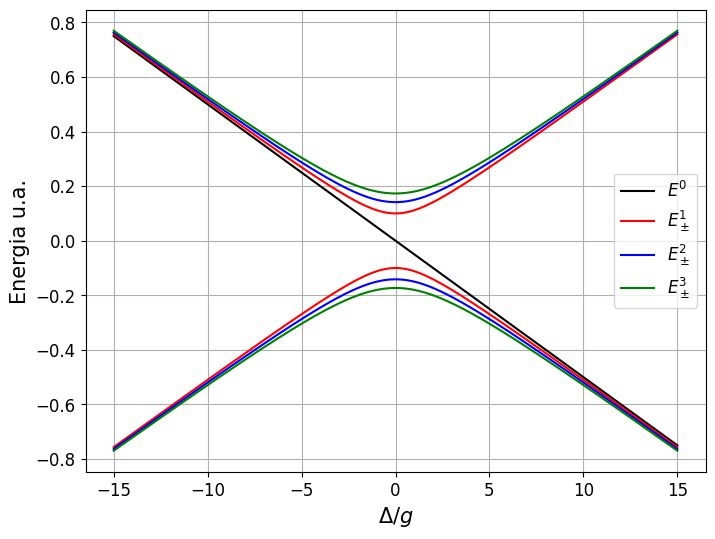
\includegraphics[width=0.7\textwidth]{figuras/ch3/relacion energia detunning jcm simple.png}
    \caption{Relaci\'on energ\'ia detunning para el modelo de Jaynes-Cummings. La diferencia de energ\'ia entre los estados de un mismo nivel para $\Delta=0$ es $2g\sqrt{n}$.}
    \label{fig:relación energia detunning jcm1}
\end{figure}
En la figura \ref{fig:relación energia detunning jcm1} se observan las curvas de energ\'ia en funci\'on del detunning para diferentes niveles. Lo primero que tenemos que observar es que en el caso resonante, es decir $\Delta=0$, los autoestados del sistema son los estados maximamente entrelazados de Bell
\begin{equation}
    \ket{\psi_\pm^n}=\frac{1}{\sqrt{2}}(\ket{gn}\pm\ket{e,n-1})
\end{equation} 
y la diferencia de energ\'ia entre los autoestados es $\Delta E^n =E^n_+-E^n_-=2g\sqrt{n}$. En el caso muy lejos de resonancia podemos asumir que $\Delta \gg g $, y entonces los autoestados coinciden en este l\'imite con los estados de la base, 
\begin{equation}
    \begin{aligned}
        \ket{\psi^n_+}=\ket{e,n-1} \\
        \ket{\psi^n_-}=\ket{g,n}
    \end{aligned}
\end{equation}
Ac\'a hay una sutileza, y es que si $\Delta>0$, entonces $\ket{e,n-1}$ es el estado de mayor energ\'ia y la notaci\'on coincide con la energ\'ia, pero si $\Delta<0$ entonces el estado $\ket{\psi^n_+}$ es el estado de menor energ\'ia. 
Un efecto interesante es que en el caso de alta desinton\'ia, podemos calcular la diferencia entre la energía del autoestado exacto del Hamiltoniano $\ket{\psi_\pm^n}$ y la energía asintotica a la que tiende, que es la energía de los estados de la base $\ket{g,n},\ket{e,n-1}$. Esta diferencia ... \textcolor{red}{VOLVER A ESTO Y VER SI DEJARLO O SACARLO. EVENTUALMENTE COMPLETAR.}
\begin{equation}
    \begin{aligned}
        \Delta E_{e,n-1}=E_+^n-E^{(0)}_{e,n-1}=\frac{g^2}{\Delta}n
        \Delta E_{g,n}=E_-^n-E^{(0)}_{g,n}=-\frac{g^2}{\Delta}n
    \end{aligned}
\end{equation}
El resultado importante de esta diferencia de energias es que aun en ausencia de fotones en la cavidad $n=0$, hay una diferencia entre las energias entre el Hamiltoniano del átomo, y del $H_{JC}$. Este efecto es el \textit{Lamb Shift} y nos dice que el vac\'io electromagnetico induce un corrimiento en la energ\'ia de los estados. Esto es importante notarlo, porque para el caso de dos átomos tambien est\'a manifiesto.

\subsection{Fase geométrica en el JCM}
Vamos a analizar la fase de Berry y la fase geométrica en la aproximación cinemática.
\subsubsection{Fase de Berry}
Para ver la fase de berry tenemos que tener un parámetro de control en el Hamiltoniano, el cual varía lentamente. Para esto necesitamos aplicar una transformación unitaria de corrimiento de fase al Hamiltoniano original \ref{eq3:hamiltoniano jcm} $R=\exp{-i\Omega a^\dagger a}$, que queda
\begin{equation}
    H=\frac{\Delta}{2}\sigma_z+g(a^\dagger \sigma_e^{-i\Omega}-+a\sigma_+e^{i\Omega})
\end{equation}
que ahora depende explicitamente del parámetro externo de control $\Omega$. Los autoestados de este nuevo Hamiltoniano se obtienen aplicando esta misma transformación sobre los autoestados del Hamiltoniano original. Si el parámetro de control varia lentamente entre 0 y $2\pi$, entonces estamos dentro de las hipotesis propuestas por Berry, y podemos calcular la fase de Berry mediante la ecuación \ref{eq2:fg berry}:
\begin{equation}
    \psi_a^n=i\oint_Cd\Omega\bra{\psi_\pm^n}R(\Omega)^\dagger \frac{d}{d\Omega}\ket{\psi_\pm^n}=\pi(1\pm \cos(\theta_n))
\end{equation}

que es no trivial incluso para $n=0$, lo que nos dice que incluso el vacio electromagnetico introduce una corrección en la fase de Berry.
\subsubsection{Aproximación Cinemática}
Para comparar ambos metodos, ahora vamos a calcular la fase geométrica utilizando la aproximación cinemática aunque este abordaje es más general de lo necesario en este caso.
Si se considera que el estado inicial es un atuoestado del Hamiltoniano, como los estados $\ket{\psi_\pm^n}$, entonces la fase geométrica en este caso se anula. Pero si se considera un estado inicial, por ejemplo $\ket{\psi(0)}=\ket{e,n}$, entonces el estado a tiempo $t$ resulta
\begin{equation}\label{eq3:fg berry jcm}
    \ket{\psi(t)}=(\cos^2\theta_ne^{-iE_+^nt}+\sin^2\theta_ne^{iE_+^nt})\ket{e,n}-i \sin\theta_n\sin(E_+^nt)\ket{g,n+1}
\end{equation}
La fase geometrica acumulada \ref{eq2:fg cinematica unitaria} es
\begin{equation}\label{eq3:fg unitaria jcm}
    \phi_u[C]=-\pi(1-\cos\theta_n)\frac{t}{T} +\arg\left\{ 1+e^{2\pi i \frac{t}{T}}\frac{\Omega_n-\Delta}{\Omega_n+\Delta} \right\}
\end{equation}
con $T=\frac{2\pi}{\Omega_n}$ es un período correspondiente a la frecuencia de Rabi $\Omega_n$. Esta expresión y la antrior \ref{eq3:fg berry jcm}, deberian coincidir cuando $t=T$, que se corresponde con un ciclo cerrado. En este caso ($t=T$) se obtiene
\begin{equation}
    \phi_u=-\pi(1-\cos\theta_n)
\end{equation}
La diferencia de signos se puede explicar comparando las curvas descritas por la esfera de Bloch para cada evolución. 
\begin{figure}[H]
    \centering
    \begin{subfigure}[h]{0.49\textwidth}
        \centering
        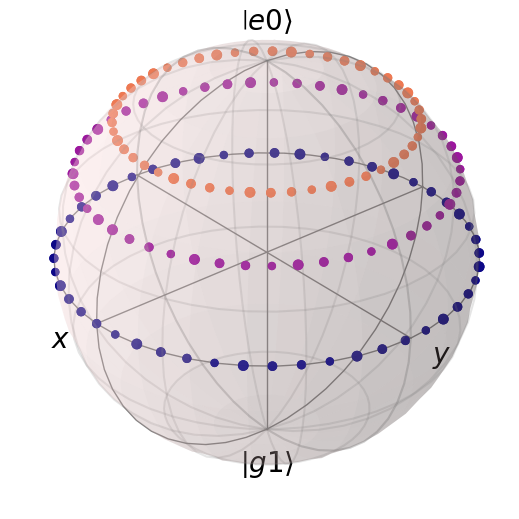
\includegraphics[width=\textwidth]{figuras/ch3/bloch berry.png}
        \caption{Evolución adiabática} 
        \label{fig3:bloch berry}
    \end{subfigure}
    \hfill
    \begin{subfigure}[h]{0.49\textwidth}
        \centering
        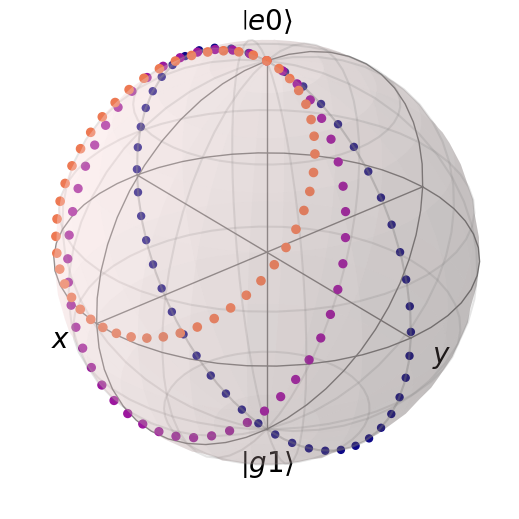
\includegraphics[width=\textwidth]{figuras/ch3/bloch cinematica.png}
        \caption{Enfoque cinemático}
        \label{fig3:bloch cinematica}
    \end{subfigure}
    \caption{}
    \label{fig3:esfera de bloch jcm}
\end{figure}
En el caso \ref{eq3:fg berry jcm}, correspondiente a la figura \ref{fig3:bloch berry}, los autoestados son los autoestados $R(\Omega)\ket{\psi_\pm^n}=e^{-i\Omega \hat n}\ket{\psi_\pm^n}$, entonces al variar $\Omega\in [0,2\pi]$ la trayectoria es simplemente un circulo en la esfera de Bloch. En cambio, en el segundo caso, si preparamos el sistema inicialmente en el estado $\ket{e,n}$ y lo dejamos evolucionar por la acción de H durante un tiempo, la trayectoria ahora no son circulos horizontales en la esfera, sino que parten del polo norte, que es el estado $\ket{e,n}$, y luego hace una trayectoria ovalada, para finalmente volver al punto inicial de partida a un tiempo $t=T$. La diferencia en el signo se explica a travez de la transformación que nos lleva de una curva a la otra. Para esto, necesitamos de una rotacion rigida, y una inversion de la parametrizacion, por su parte, esta ultima, introduce un signo negativo, cosa que se ve claramente en la ecuacion \ref{eq3:fg unitaria jcm} al cambiar $t\rightarrow -t$.

\textcolor{red}{aca puedo intentar de agregar el caso con medio kerr. Creo que no es tan complicado y el problema de autocosas ya lo tengo medio resuelto en papel desde hace un tiempo, pero lo tengo que revisar a ver si esta bien y lo tengo que completar, pero puede estar bueno para entender que le hace a la FG desde el vamos.}

\section{JCM disipativo}


Habiendo desarrollado el análisis de la fase geométrica acumulada por el sistema átomo-cavidad en la situación ideal de completo aislamiento, se aborda ahora el estudio para el escenario más realista en el que el mismo sistema se encuentra en interacción con un entorno. El problema se trata para la implementación específica en estructuras semiconductoras, en las que un punto cuántico (al cual se sigue, sin embargo, refiriendo como átomo o sistema de dos niveles) se ubica en una nano o micro-cavidad.

Siguiendo \cite{80}, en este capítulo se estudia en detalle la fase geométrica acumulada en un modelo de Jaynes-Cummings disipativo, como caso paradigmático dentro del campo de la electrodinámica en cavidades. Se considera que los principales mecanismos por los cuales el sistema “átomo + modo” interactúa con el entorno son el flujo de fotones a través de las paredes de la cavidad y el continuo e incoherente bombeo del sistema de dos niveles, lo que conforma un escenario frecuente en electrodinámica de cavidades semiconductoras \cite{81,82,83}. 

Para poder modelar estos mecanismos, se emplea la ecuación maestra fenomenológica de Lindblad
\begin{equation}\label{eq3:lindblad}
\dot{\rho}(t) = -i [H, \rho(t)] + \frac{1}{2} \sum_\alpha \big( 2L_\alpha \rho(t) L_\alpha^{\dagger} - \{ L_\alpha^{\dagger}L_\alpha, \rho(t) \} \big),
\end{equation}

, despreciando otros procesos con menor influencia en la dinámica como el desfasaje puro o el bombeo de fotones del entorno en la cavidad, considerando además que el entorno se halla a temperatura cero. Los operadores de Lindblad

\begin{equation}
L_\gamma = \sqrt{\gamma} \ a
\end{equation}
\begin{equation}
L_p = \sqrt{p} \ \sigma_+
\end{equation}

,representan la pérdida de fotones y el bombeo continuo e incoherente del átomo, respectivamente, con los parámetros $\gamma$ y $p$ denominados tasa de pérdida de fotones y amplitud del bombeo. 

El bombeo sobre el átomo es siempre secundario frente a la pérdida de fotones, lo cual nos da las relaciones $\frac{p}{g},\frac{p}{\gamma} \ll 1$, y la relación entre $\gamma$ y $g$ da lugar a dos regimenes que se diferencian con claridad \cite{50}-\cite{54}. El regimen de acoplamiento fuerte (SC o Strong Coupling) es cuando la interacción átomo-cavidad es mas fuerte que la disipación del entorno, es decir $\gamma /g <1$. En el caso contrario $\gamma/g>1$ estamos en el régimen de acoplamiento débil (WC o Weak Coupling). Para no generar confusiones, hay que destacar que en general, cuando en la literatura se habla de acoplamientos fuertes y debiles, se refiere a la interacción entre las partes del mismo sistema, pero en este caso, se esta haciendo referencia a la interacción del sistema con el entorno EN COMPARACIÓN con la interacción interna del sistema.

En esta ocación nos interesa resolver el problema restringiendonos al subespacio donde el átomo puede estar en cualquiera de sus dos estados, y nos restringimos al caso en donde la cavidad tiene 1 o 2 fotones, en consecuencia, se restringe el estudio a un subespacio truncado cuya base son los estados $\{ \ket{0}=\ket{g,0} ; \ket{1}=\ket{e,0} ; \ket{2}=\ket{-,1} \}$. Desarrollando explicitamente el sistema de ecuaciones dadas por la ecuación de Lindblad \ref{eq3:lindblad}, obtenemos que los elementos $\rho_{0i}$ quedan desacoplados de los demas:

\begin{equation}
    \begin{aligned}
        \dot \rho_{01} & =-\frac{p}{2} \rho_{01}+i\Delta\rho_{01}+ig\rho_{02} \\
        \dot \rho_{02} & =-\frac{p}{2} \rho_{02}-\gamma \rho_{02}+ig\rho_{01}
    \end{aligned}
\end{equation}
,con lo cual, si inicialmente los elementos de matriz $\rho_{0i}(0)=0$, permanecerán así durante toda la evolución del sistema. Para hacer una analogía y realizar una comparación con el caso unitario, se estudia la condición inicial $\rho(0)=\ketbra{e,0}{e,0}$, que satisface esta condición, de manera que se espera que el estado $\rho(t)$ exciba una estructura diagonal por bloques. El primer bloque de 1x1 representando al estado $\ket{0}$, y luego un bloque de 2x2 que describe la dinámica entre los estados $\ket{1}$ y $\ket{2}$. Las ecuaciones son
\begin{equation}
\begin{aligned}
\dot{\rho}_{00} &= -p \rho_{00} + \gamma \rho_{22}, \\
\dot{\rho}_{11} &= -i g (\rho_{21} - \rho_{12}) + p \rho_{00}, \\
\dot{\rho}_{22} &= -i g (\rho_{12} - \rho_{21}) - \gamma \rho_{22}, \\
\dot{\rho}_{12} &= -i g (\rho_{22} - \rho_{11}) - i \Delta \rho_{12} - \frac{\gamma}{2} \rho_{12}.
\end{aligned}
\end{equation}

que se resuelven numericamente para acceder al estado $\rho(t)$ a tiempo $t>0$. 

\textbf{[Placeholder para Figura: Evolución dinámica de elementos de matriz]}

El análisis de esta sección permite establecer la relación entre los efectos de disipación y la acumulación de la fase geométrica, así como determinar las condiciones bajo las cuales el sistema mantiene coherencia cuántica suficiente para aplicaciones experimentales.

	\chapter{Jaynes-Cummings de dos átomos con medio y acoplamiento no lineal}
\label{ch4_dinamica}

%CAMBIAR ESTO PARA PERSONALIZARLO A MI GUSTO
\pagestyle{fancy}
\fancyhf{}
\fancyhead[LE]{\nouppercase{\rightmark\hfill}}
\fancyhead[RO]{\nouppercase{\leftmark\hfill}}
\fancyfoot[LE,RO]{\hfill\thepage\hfill}

En este capítulo se extiende el modelo de Jaynes-Cummings presentado en el capítulo \ref{ch3_jcm}. Lo más importante es que ahora se tienen dos átomos dentro de una misma cavidad. En la literatura en general, el modelo de JC fue extendido para considerar dos cavidades donde cada una tiene su propio átomo, y usando una condición inicial entrelazada se puede hacer interactuar ambas cavidades. El camino que se toma en este trabajo, es un tanto fuera de lo convencional, ya que no hay muchos estudios sobre este sistema. El principal obstáculo que presenta este problema, es que el espacio de Hilbert se duplica con respecto al caso de 1 átomo, y se torna inmanejable analíticamente. Como bien es sabido, el JCM tiene subespacios de 2 dimensiones que no se mezclan. Utilizando esta estrategia pero con dos átomos, se tendrán subespacios de 4x4 que tampoco se mezclan en el caso unitario. Esto permite encontrar algunas expresiones analíticas, pero en general se utilizarán métodos numéricos para analizar la dinámica. \newline
Este capítulo entonces seguirá un hilo conductor, partiendo desde el caso más sencillo hasta llegar a analizar cuáles son los efectos de los diferentes parámetros en el problema, y particularmente se considerarán los efectos que éstos tienen sobre la dinámica de entrelazamiento entre los dos átomos. 
Primero se resolverá el problema unitario de manera exacta, y se analizarán las energías. Luego, para comprender las partes del problema, se aislará uno de los dos átomos, haciéndolo invisible a las interacciones con el otro átomo y con la cavidad. El objetivo de esto será recuperar numéricamente los resultados del capítulo anterior. Al terminar ese análisis, se continuará prendiendo las interacciones del átomo que se aisló del sistema, volviendo al problema completo. En este contexto se estudiará la dinámica poblacional y principalmente la dinámica de entrelazamiento entre los dos átomos. Para esto es necesario trazar sobre la cavidad, obteniendo así una matriz densidad reducida que solo tiene en cuenta la dinámica de los dos átomos. Los efectos de la cavidad estarán entonces contemplados de manera efectiva, y no implícita. El efecto que tienen las interacciones del problema sobre el entrelazamiento entre los átomos, será la última parte de este capítulo.
%Primero se considera una cavidad perfecta, es decir sin disipaci\'on, agregándole el segundo átomo, vamos a intentar de entender cual es el efecto de este sobre el modelo de un solo átomo. Para esto haremos un análisis poblacional, y de observables como la entropía reducida, la concurrencia, las matrices de Pauli. Una vez agregado el segundo átomo, vamos a prender las interacciones de a una y vamos a analizar cuales son sus efectos. Luego, vamos a comparar esto con el caso en donde la cavidad presenta pérdidas. Principalmente, nos centraremos en un análisis del entrelazamiento, ya que esta es la cualidad más interesante que tenemos en el ámbito de la informaci\'on cu\'antica. 



\section{Modelo de dos átomos y solución unitaria}
Este trabajo se concentra en una extensión del modelo, donde se ubican dos átomos dentro de la cavidad. Estos átomos pueden interactuar entre sí, y con la cavidad, y además se consideran no-linealidades en el acoplamiento y en el medio.
Se utiliza un modelo de Jaynes-Cummings para describir la interacci\'on entre el campo electromagn\'etico y los átomos. Adem\'as se supondrá que el acoplamiento depende de la cantidad de fotones y los átomos podr\'an interactuar entre sí mediante un término tipo Ising y otro tipo dipolo-dipolo. Recordemos que se asume que vale la aproximaci\'on de onda rotante ($\omega_0 \sim \omega$) y $g << \omega,\omega_0$.
Entonces, el Hamiltoniano que describe este problema es el siguiente ($\hbar=1$):
\begin{equation}
\begin{split}
     \hat H & =\underbrace{ \omega_0 h(\hat n) \hat n }_{\hat H_F}+\underbrace{\frac{ \omega}{2}(\hat\sigma_Z^{(1)}+\hat\sigma_Z^{(2)})}_{\hat H_A}   \\ 
     & + \underbrace{ g(\hat\sigma_+^{(1)}\hat a f(\hat n)+\hat\sigma_-^{(1)}f(\hat n) \hat a^\dagger + \hat\sigma_+^{(2)}\hat a f(\hat n)+\hat\sigma_-^{(2)}f(\hat n) \hat a^\dagger)}_{H_{FA}} \\ +& \underbrace{2 \kappa (\hat \sigma_-^{(1)}\hat \sigma_+^{(2)}+\hat \sigma_+^{(1)}\hat \sigma_-^{(2)}) +  J \hat \sigma_Z^{(1)}\hat \sigma_Z^{(2)}}_{H_{AA}},
\end{split}
\end{equation}
donde $\hat a$ es el operador de aniquilaci\'on del fot\'on, $\omega_0$ y $\omega$ son las frecuencias del fot\'on y del átomo respectivamente (ambos átomos en la cavidad tienen la misma frecuencia natural para simplificar el problema), $g$ es la constante de acoplamiento, las constantes $J$ y $\kappa$ son los par\'ametros de Ising y de dipolo-dipolo para las interacciones átomo-átomo, y los operadores $\hat \sigma^{(i)}$ son las matrices de Pauli que act\'uan sobre el átomo i-esimo. Finalmente, las funciones $h(\hat n)$ y $f(\hat n)$ son las que dan cuenta de la no linealidad dependiente del número de fotones de la cavidad $\hat n = \hat a^\dagger \hat a$. 

Un medio tipo Kerr está descrito por la funci\'on $h(\hat n)=1+\frac{\chi}{\omega_0}\hat n$ \cite{Lugiato1987}, y la funci\'on $f(\hat n)$ describe el tipo de acoplamiento, de las cuales se consideran dos opciones: si el acoplamiento es lineal $f(\hat n)=1$, y si el acoplamiento es no lineal, específicamente se considera de tipo Buck-Sukumar $f(\hat n) = \sqrt{\hat n}$ \cite{Buck1980}.

En este punto es útil hacer una transformaci\'on unitaria  $K = \exp\left\{-i \omega t (\hat a^\dagger \hat a + \hat \sigma_z/2)\right\}$ para dejar el Hamiltoniano en funci\'on del detunning $\Delta (\sim 0)$. 

\begin{equation}
\begin{split}
     \hat H_I & = \chi \hat n^2+\frac{ \Delta}{2}(\hat\sigma_Z^{(1)}+\hat\sigma_Z^{(2)})   \\ 
     & +  g(\hat\sigma_+^{(1)}\hat a f(\hat n)+\hat\sigma_-^{(1)}f(\hat n) \hat a^\dagger + \hat\sigma_+^{(2)}\hat a f(\hat n)+\hat\sigma_-^{(2)}f(\hat n) \hat a^\dagger) \\ 
 & + 2 \kappa (\hat \sigma_-^{(1)}\hat \sigma_+^{(2)}+\hat \sigma_+^{(1)}\hat \sigma_-^{(2)}) +  J \hat \sigma_Z^{(1)}\hat \sigma_Z^{(2)}.
\end{split}
\end{equation}\label{ec4:H}
Este es el Hamiltoniano con el que se trabaja, así que a partir de ahora el subíndice I es redundante y se dejará implícito. Obsérvese que el caso de $\chi=0$ es el caso de un medio lineal. 


Este Hamiltoniano se puede resolver analíticamente para el caso de una cavidad sin pérdidas \cite{Santos2016}. Lo primero que se nota es que el Hamiltoniano conserva el número de excitaciones, es decir $[H,\hat N]=0$, y en esta situación es sabido que el Hamiltoniano de JC es diagonal por bloques si se elige convenientemente la base. Esta es la que agrupa los estados con misma cantidad de excitaciones $\hat N = \hat n + \hat \sigma_+^{(1)}\hat \sigma_-^{(1)}+\hat \sigma_+^{(2)}\hat \sigma_-^{(2)}$: 
\begin{equation}
\begin{split}
    \mathcal{B}_n=& \left\{\ket{\Phi^{(n)}_1}=\ket{gg,n},\ket{\Phi^{(n)}_2}=\frac{1}{\sqrt{2}}(\ket{eg,n-1}+\ket{ge,n-1}),\ket{\Phi^{(n)}_3}=\ket{ee,n-2},\right. \\
& \left. \ket{\Phi^{(n)}_4}=\frac{1}{\sqrt{2}}(\ket{eg,n-1}-\ket{ge,n-1})\right\} ,
\end{split}
\label{ec4:base}
\end{equation}
donde se eligi\'o esta combinaci\'on particular, porque el último estado de la base, que es impar ante intercambio, queda desacoplado de los otros. Esto se ve al evaluar los elementos de matriz del Hamiltoniano $H_{i,j}=\bra{\Phi_i}\hat H \ket{\Phi_j}$. El subespacio correspondiente a $n$ excitaciones $\hat H^{(n)}$ es una matriz de 4x4
\begin{equation}
    \hat H^{(n)}=
    \begin{pmatrix}
     \chi n^2 - \Delta +  J & \sqrt{2} g f(n)\sqrt{n} & 0 & 0 \\
    \sqrt{2} g f(n)\sqrt{n} &  \chi (n-1)^2  -  J + 2 k & \sqrt{2} g f(n-1)\sqrt{n-1} & 0 \\
    0 & \sqrt{2} g f(n-1)\sqrt{n-1} &  \chi (n-2)^2 +  \Delta +  J & 0 \\
    0&0&0& \begin{aligned} 
                 & \chi (n-1)^2  \\ 
                 &-  J - 2 k
        \end{aligned}
    \end{pmatrix}.
\end{equation}
Claramente, el estado impar ante intercambio está aislado, y entonces es autoestado del problema. Por lo tanto evoluciona sólo y no se mezcla con los otros estados. Entonces, para terminar de resolver el problema, hay que diagonalizar la matriz de 3x3. Cabe aclarar que esta matriz solo es válida para una cantidad de excitaciones $N\geq 2$, ya que los subespacios con $0$ o $1$ excitación no tienen 4 estados. En estos casos la soluci\'on del problema de autovalores es más sencilla aún, as\'i que solo se mostrarán los resultados. \newline
Para resolver el problema de autovalores de la matriz de 3x3 se utiliza la fórmula de Cardano para conseguir las ra\'ices triples que aparecen en el polinomio caracter\'istico, cuyos autovalores son
\begin{equation}
    E_j^{(n)}=-\frac{1}{3}\beta_n+2\sqrt{-Q_n}\cos{\left(\frac{\theta_n+2(j-1)\pi}{3}\right)},
    \label{ec4:autoenergias}
\end{equation}
para $j=1,2,3$, y donde:
\begin{equation}
    \theta_n=\cos^{-1}\left(\frac{R_n}{\sqrt{-Q_n^3}}\right),
\end{equation}
\begin{equation}
    \begin{aligned}
        Q_n & = \frac{3\gamma_n-\beta_n^2}{9} ,\\
        R_n & = \frac{9\beta_n\gamma_n-27\eta_n-2\beta_n^3}{54} ,\\
        \beta_n & = - \left( \chi(n^2+(n-1)^2+(n-2)^2)+J+2k\right) ,\\
        \gamma_n & = (\chi(n-1)^2 - J + 2k)(x(n-2)^2+\chi n^2+2J) \\ 
        & +(\chi (n-2)^2+\Delta+J)(x n^2-\Delta+J)-2g^2(n^{2a}+(n-1)^{2a}) ,\\ 
        \eta_n &= -(\chi n^2-\Delta+J)(\chi(n-2)^2+\Delta+J)(\chi(n-1)^2-J+2k) \\
        &+2g^2 \left[  \chi(n-2)^2n^{2a}+\chi n^2(n-1)^{2a}+\Delta\left(n^{2a}-(n-1)^{2a}\right) +J(n^{2a}+(n-1)^{2a})\right].
    \end{aligned} 
    \label{ec4:parametros solucion}
\end{equation}
donde $a=\frac{1}{2}$ se corresponde con acoplamiento lineal, es decir, $f(n)=1$, y $a=1$ a Buck-Sukumar $f(n)=\sqrt{n}$. Los autovalores son reales si $Q_n^3+R_n^2<0$.
Con esto podemos escribir los autovectores:
\begin{equation}
    \begin{split}
        \ket{u_j^{(n)}} &= \frac{1}{N_j^{(n)}} \bigg[ \left((E_j^{(n)} - H_{22}^{(n)})(E_j^{(n)}-H_{33}^{(n)}) - H_{23}^{(n)^2} \right) \ket{\Phi_1^{(n)}} \\ &+ H_{21}^{(n)}(E_j^{(n)}-H_{33}^{(n)})\ket{\Phi_2^{(n)}} + H_{23}^{(n)}H_{12}^{(n)}\ket{\Phi_3^{(n)}}\bigg].
    \end{split}
\end{equation}
Obviamente el último es el estado $\ket{\Phi_4^{(n)}}$, que también es autoestado, con autovalor $E_4^{(n)}=\chi(n-1)^2-J-2k$.
Para el subespacio de $N=0$ solo hay un vector $\ket{\Phi_1^{(0)}}=\ket{gg0}$ y su autovalor es $E_1^{(0)}=-\Delta+J$.
Para $N=1$ se tienen tres vectores en el subespacio, y las autoenergías son
\begin{align}\label{ec4:energias n1}
    E_{1,2}^{(1)} &=\frac{\chi -\Delta}{2} +k \pm \sqrt{2g^2+(k-J+\frac{\Delta -\chi}{2} )^2},\\
    E_3^{(1)} & = -2k-J,  
\end{align}
y sus autovectores
\begin{equation}
    \begin{aligned}
        \ket{u_{1,2}^{(1)}}&=\frac{1}{N_{1,2}^{(1)}}(-\sqrt{2}g\ket{gg1}+ \left(\frac{\chi-\Delta}{2}+J-k \mp \sqrt{2g^2+(k-J+\frac{\Delta -\chi}{2} )^2} \right)\dfrac{\ket{eg0}+\ket{ge0}}{\sqrt{2}},\\
        \ket{u_3^{(1)}}&= \frac{1}{\sqrt{2}}(\ket{eg0}-\ket{ge0}).
    \end{aligned}
\end{equation}

Con esto, se resuelve analíticamente la evolución temporal de cualquier estado inicial.
Para esto sólo es necesario desarrollar el estado inicial en términos de los autovectores, y la evolución temporal está dada por
\begin{equation}
\ket{\psi(t)}=e^{-iHt}\ket{\psi(0)}=\sum_{j,n} c_j^{(n)}e^{-iE_j^{(n)}t}\ket{u_j^{(n)}},
\end{equation}
donde $c_j^{(n)}=\braket{u_j^{(n)}}{\psi(0)}$.
La complejidad de estas expresiones hace difícil conseguir conclusiones interesantes, aun así, algo que se puede notar, es la diferencia fundamental entre las energías con un número total de excitaciones $N=1$ y $N>1$. Hay un factor antes de la raíz cuadrada, que para el caso en que $N \geq 2$ es $\frac{1}{3}\beta_n$ que sólo depende de $\chi$, $J$, $k$ y $n$. Mientras que en el caso de $N=1$, este factor depende del detunning $\Delta$. Esto es interesante, ya que uno podría pensar que la fórmula para $N$ excitaciones se puede generalizar para incluir $N=0,1$, pero la diferencia fundamental de tener más o menos estados que interactúan entre sí, da lugar a efectos fundamentalmente diferentes. Más en detalle, en el caso de $N=1$ este factor $\Delta$ aparece, ya que en la matriz Hamiltoniana el único estado con $N=1$ que tiene un término que incluye al detunning, es el estado $\ket{gg1}$. Por lo tanto, este término con $\Delta$ sobrevive, al contrario que en todos los demás subespacios, ya que por un lado el término del $\ket{ggn}$ que aporta un $\Delta$, y el término de $\ket{ee,n-2}$ aporta otro $\Delta$ pero con el signo cambiado, y elimina la contribución del primer estado a la energía. La consecuencia de esto es que para $N=1$, si se aumenta el detunning, no sólo se separan los niveles de energía, sino que también hay una asimetría por el término independiente. Para analizar ésto en detalle, en la figura \ref{fig:relación energia detunning} se observan las energías de los diferentes niveles en función del detunning. 

\begin{figure}
    \centering
    \begin{subfigure}[h]{0.49\textwidth}
        \centering
        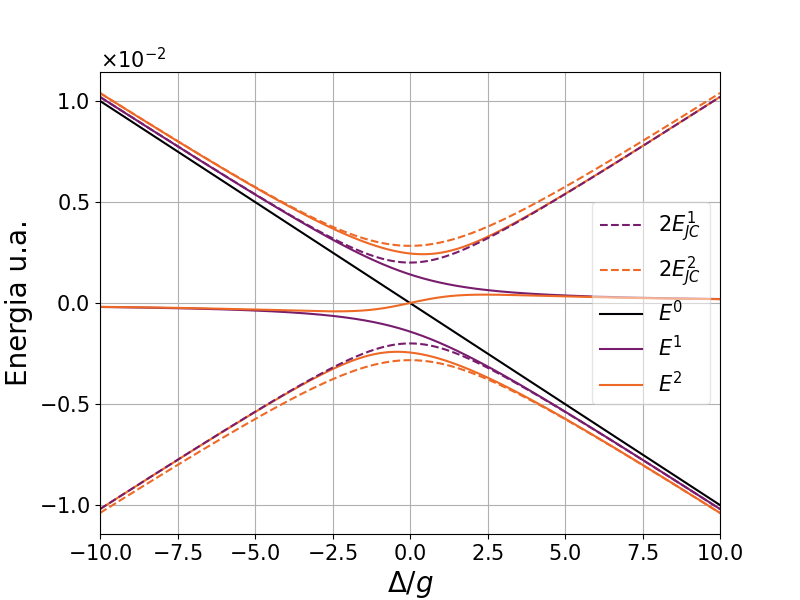
\includegraphics[width=\textwidth]{figuras/ch4/energias 0.png}
        \caption{}
        \label{fig:relación energia detunning 1}
    \end{subfigure}
    \hfill
    \begin{subfigure}[h]{0.49\textwidth}
        \centering
        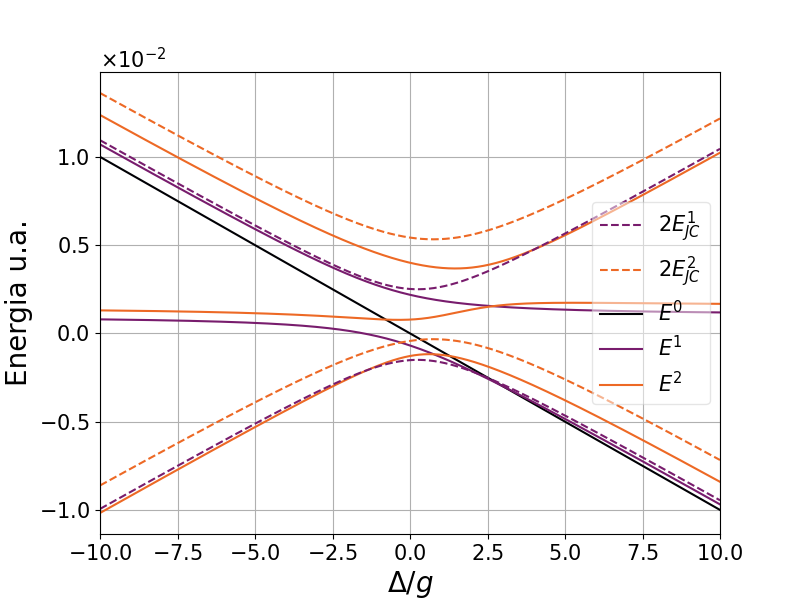
\includegraphics[width=\textwidth]{figuras/ch4/energias 0.5.png}
        \caption{}
        \label{fig:relación energia detunning 2}
    \end{subfigure}
       \caption{Relación entre energía y detunning para los diferentes niveles de energía del problema. Las líneas sólidas muestran la energía de los estados del JC de dos átomos con una cantidad de excitaciones: $N=0$ (negro, sólido), $N=1$ (violeta sólido) y $N=2$ (naranja sólido). También se muestran los niveles de energía del JC de un átomo para $N=1$ (negro; rayado) y $N=2$ (naranja; rayado). Obsérvese que las energías del JC de un átomo están multiplicadas por 2. (a) $\chi=k-J=0$; (b) $\chi=k-J=0.5g$}
       \label{fig:relación energia detunning}
\end{figure}
En la figura \ref{fig:relación energia detunning 1} se observan las energías de los primeros niveles para el modelo de un átomo (líneas rayadas), y de dos átomos (líneas sólidas). Para esta figura se tomaron átomos que no interactúan ($k=J=0$) y una cavidad lineal ($\chi=0$). Se puede ver que, si bien el modelo de dos átomos tiene estructuras más complicadas, son similares a las de 1 átomo. En primer lugar, los estados con $N=2$ (naranja; sólido) tienen una forma igual a la de JC de 1 átomo, si bien está un poco desfasada, es interesante ver como las líneas tienen una coincidencia muy grande. Recordando que en el gráfico las líneas rayadas están multiplicadas por 2, esto tiene una interpretación bastante buena, y es que la energía de dos átomos no interactuantes en una cavidad es igual (o muy parecida) a dos veces la energía de 1 átomo en una cavidad. Esta diferencia se debe al corrimiento Lamb, ya que ahora al tener dos átomos que interactúan con el vacío, tiene una forma un poco diferente:
\begin{equation}
    \begin{aligned}
        \Delta E_{1}&=E^{n}_1-E^{(0)}_1=\frac{2g^2}{\Delta}(2n-1), \\
        \Delta E_{2}&=E^{n}_2-E^{(0)}_2=-\frac{2g^2}{\Delta}(2n-1), \\
        \Delta E_3 &=0 .
    \end{aligned}
\end{equation}
Las tres autoenergías presentan correcciones del orden de $\frac{g^2}{\Delta}$ en su valor asintótico, pero la dependencia cambia con respecto al caso de 1 átomo, lo que explica las diferencias de la figura \ref{fig:relación energia detunning 1}. Esta dependencia es sorprendente ya que no es simplemente el doble que el caso de 1 átomo. En la figura \ref{fig:relación energia detunning 2}, donde hay interacción entre átomos, se pierde la analogía con el caso de 1 átomo.

Por otro lado, la energ\'ia de los estados con $N=1$ tienen un t\'ermino fuera de la raíz, que hace que sea más asim\'etrico a\'un. Normalmente, en el JC de 1 átomo, ya que todos los niveles de energía tienen la misma forma funcional, este término de afuera de la raíz se le puede agregar o quitar como un offset en la energía del estado fundamental. La diferencia con este caso es que no todos los niveles de energía presentan esto, entonces si se agrega un offset, igualmente habría una diferencia. 

Una observación menor es que si la cavidad es lineal, entonces los estados antisimétricos de diferentes excitaciones $\frac{1}{\sqrt{2}}(\ket{eg,n}-\ket{ge,n})$ y $\frac{1}{\sqrt{2}}(\ket{eg,n'}-\ket{ge,n'})$, están degenerados en energía. Esto solo tiene importancia al considerar una cavidad con pérdidas.

Una vez estudiados los niveles de energía y comparados con el caso de 1 átomo, se prosigue con la dinámica del problema, que en el caso unitario puede resolverse analíticamente, pero a\'un así, la herramienta principal de análisis son las simulaciones numéricas.
Para comenzar se quiere recuperar el caso de un átomo. Para esto se trabaja con $k=J=0$ y se agrega un parámetro adimensional $\alpha$ que solamente actúa sobre el átomo B, y sirve de apantallamiento. Este parámetro $\alpha$ acompaña a las constantes de acoplamiento $g\rightarrow g\alpha$, tal que si $\alpha \rightarrow 0$ entonces el átomo se desacopla de la cavidad. 

\section{Dinámica con apantallamiento}
\label{sec4:dinamica apantallamiento}
Lo primero que buscamos es recuperar los resultados anteriores para un solo átomo para estar seguros de la extensión posterior a dos átomos acoplados. Para aclarar, en la figura \ref{fig4:diagrama esquematico} se muestra un esquema de cómo es el problema que se está trabajando, con los nombres que se le dan a las partes del sistema. Llamaremos átomo B al que está apantallado mediante el parámetro adimensional $\alpha$, el índice A se refiere al otro átomo, y C a la cavidad. Entonces, para recuperar los resultados anteriores, se propone que $\alpha=0$ y la interacción entre los átomos $k=J=0$. De esta manera, se elige en analogía con el caso de 1 átomo, como estado inicial cualquier estado donde el átomo A esté excitado, y la cavidad C no tenga ningún fotón; por lo tanto se elige el estado inicial más sencillo posible que cumple estas condiciones $\ket{\psi_0}=\ket{eg0}$. Si bien este apantallamiento no tiene un significado físico, y experimentalmente sería en principio, muy difícil de generar, realizar este estudio sirve para comprender cualitativamente los efectos de cada parámetro del problema, y también, entender que el entrelazamiento entre los dos átomos lleva a efectos impredecibles. La complejización del problema de 1 átomo al de 2 átomos es muy grande, y por eso es necesario ir de a poco.
\begin{figure}[h]
    \centering
    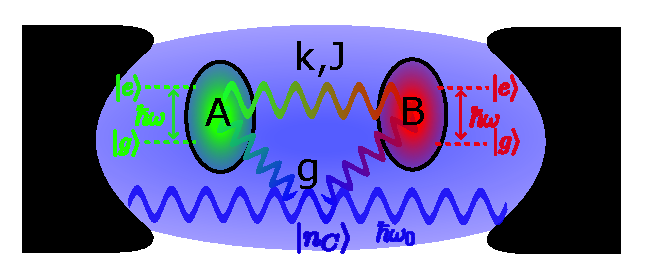
\includegraphics[width=0.74\textwidth]{figuras/ch4/esquema.pdf}
    \caption{Esquema del problema de estudio. Se nombran a las partes para referenciarlas fácilmente: los átomos se identifican por las letras A y B, y la cavidad por la C, esta puede contener una cantidad arbitraria de excitaciones, pero se trabajará principalmente en 0,1 y 2 excitaciones. Ambos átomos son de dos niveles, son idénticos e indistinguibles y su frecuencia natural es $\omega$, mientras que la frecuencia natural de la cavidad es $\omega_0$. El acoplamiento entre la cavidad y el átomo es $g$, y las interacciones átomo-átomo son $k$ (interacción dipolar) y $J$ (interacción tipo Ising).}
    \label{fig4:diagrama esquematico}
\end{figure}
Utilizando esta condición inicial se realiza una simulación numérica y se observan las poblaciones. Se espera recuperar la misma dinámica que en el caso de 1 átomo, ya que el átomo B no interactúa con ninguna de las otras partes del sistema A y C. Para poder representar el estado del sistema sobre una esfera de Bloch, se realiza una traza parcial sobre el átomo B, y así se obtiene la figura \ref{fig4:bloch delta eg0}, donde se muestran tres trayectorias correspondientes a diferentes valores del detunning. Los puntos azules son el caso resonante $\Delta=0$, la morada y naranja se corresponden con $\Delta=0.5g$ y $\Delta=2g$ respectivamente.
\begin{figure}[H]
    \begin{minipage}[c]{0.5\textwidth}
        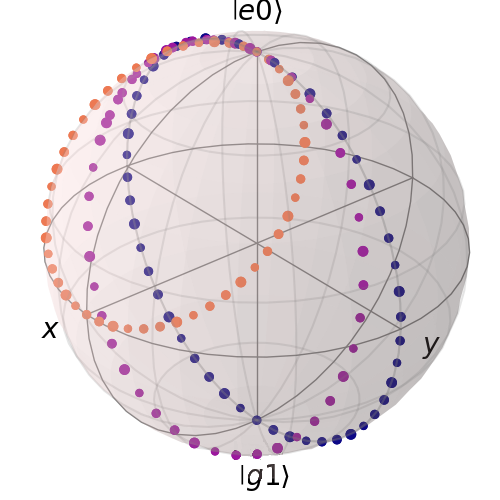
\includegraphics[width=\textwidth]{figuras/ch4/bloch eg0 bloch AC a=0 d=2.0 x=0.0 k=0.0 J=0.0 gamma=0.0 p=0.0.png}
    \end{minipage}\hfill
    \begin{minipage}[c]{0.3\textwidth}
        \caption{Trayectorias sobre la esfera de Bloch cuya condición inicial es $\ket{e_Ag_B0_C}$ para diferentes valores del detunning, apantallando el átomo B. Los valores son $\Delta=0$ (azul), $\Delta=0.5g$ (morada) y $\Delta=2g$ (naranja).}
        \label{fig4:bloch delta eg0}
    \end{minipage}
\end{figure}
Se observa como la dinámica entre estos dos estados es exactamente igual que la observada en la figura \ref{fig3:bloch cinematica}, además, como todos los puntos están sobre la superficie de la esfera, los estados son puros y entonces el estado global es separable. Haber trazado sobre el átomo B no tuvo efecto sobre la dinámica entre el átomo A y la cavidad. Para corroborar esto se realiza un análisis poblacional más profundo.
Para ello consideramos una condición inicial entrelazada. Si bien los átomos no interactúan (el átomo B está aislado del universo) se puede pensar que en algún momento los átomos se entrelazaron y luego se apagan las interacciones con el átomo B. Por ejemplo, si se considera el estado inicial entrelazado $\ket{\psi_0}=\frac{1}{\sqrt{2}}(\ket{eg0}+\ket{ge0})$, se obtienen las trayectorias mostradas en la igura \ref{fig4:bloch delta eg0 sim}.
\begin{figure}[H]
    \begin{minipage}[c]{0.5\textwidth}
        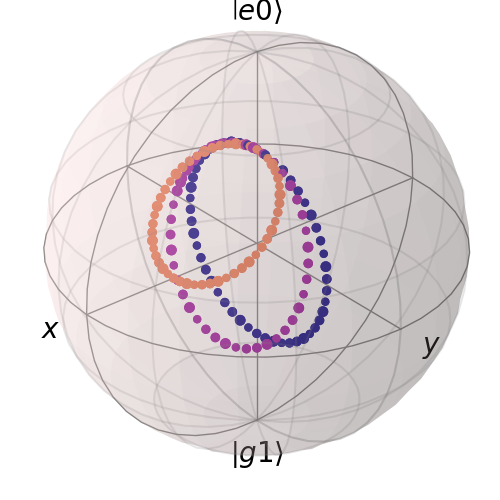
\includegraphics[width=\textwidth]{figuras/ch4/bloch eg0+ge0 bloch AC a=0 d=2.0 x=0.0 k=0.0 J=0.0 gamma=0.0 p=0.0.png}
    \end{minipage}
    \hfill
    \begin{minipage}[c]{0.3\textwidth}
        \caption{Trayectorias sobre la esfera de Bloch cuya condición inicial es $(\ket{e_Ag_B0_C}+\ket{g_Ae_B0_C})/\sqrt{2}$ para diferentes valores del detunning, apantallando el átomo B. Los valores son $\Delta=0$ (azul), $\Delta=0.5g$ (morada) y $\Delta=2g$ (naranja).}
        \label{fig4:bloch delta eg0 sim}
    \end{minipage}
\end{figure}
Ahora, los estados no están sobre la superficie, lo que se interpreta como que estamos en presencia de un estado mixto. Al trazar sobre el átomo B, efectivamente se considera como si éste fuese parte de un entorno. Al olvidarse de la dinámica del segundo átomo, se puede interpretar como que este se lleva un 50\% de probabilidad de estar excitado, ya que no sabemos si inicialmente el átomo A o el átomo B es el que tiene la excitación. Entonces efectivamente tenemos un 50\% de probabilidad de que el estado de la cavidad sea $\ket{g0}$, y no evoluciona, y un 50\% de probabilidad de que la excitación este dentro de la cavidad, y por lo tanto vemos que la dinámica es la misma que en el caso anterior, pero con amplitudes menores.

Para analizar más en detalle la dinámica, y para poder realizar comparaciones cuando se complejiza el problema, se puede realizar un estudio poblacional, y también podemos mirar las entropías relativas y otros observables importantes.
En primer lugar, el caso separable $\ket{\psi_0}=\ket{eg0}$, es idéntico al caso de 1 átomo, ya que el átomo B no evoluciona por estar totalmente aislado del sistema. Lo único que se puede resaltar es que, si se traza sobre la cavidad, que es algo útil para observar el entrelazamiento entre los átomos, entonces el estado es mixto, ya que la evolución temporal del sistema átomo A-átomo B consta del átomo B en el estado fundamental $\ket{g}$, y el átomo A oscila entre el estado excitado y fundamental. La amplitud de oscilación y el grado de \textit{mixing} entre los estados depende del detunning, siendo el caso $\Delta=0$ el de oscilaciones coherentes entre estados, y al aumentar $\Delta$ se atenúa este comportamiento.
En segundo lugar, cuando el estado inicial de los átomos no es separable por estar entrelazados $\ket{\psi_0}=\frac{1}{\sqrt{2}}(\ket{eg0} + \ket{ge0})$, entonces la dinámica es un poco diferente. La figura \ref{fig4:dinamica eg0 sim resonante} muestra el caso de $\Delta=0$, donde se observan las evoluciones de las diferentes partes del sistema.

\begin{figure}[h]
    \centering
    \begin{subfigure}{0.49\textwidth}
        \centering
        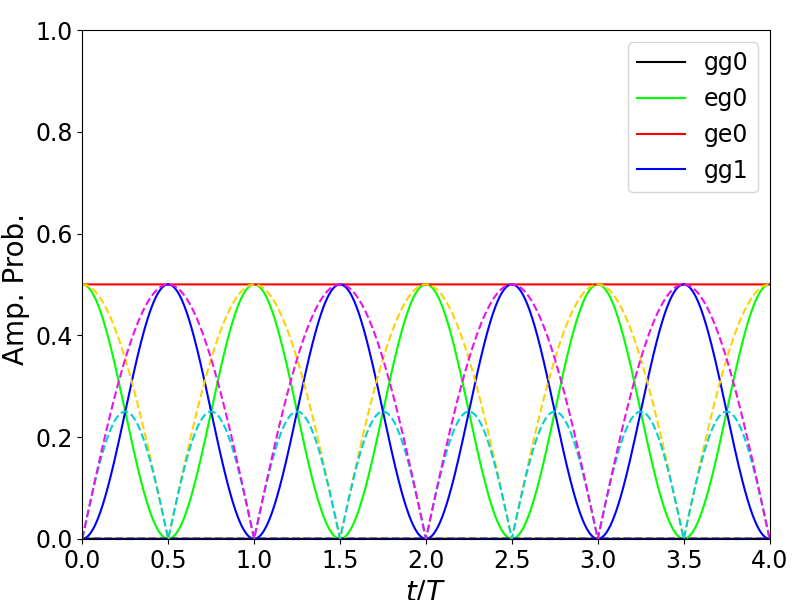
\includegraphics[width=\textwidth]{figuras/ch4/d eg0+ din ABC d=0.png}
        \caption{}
        \label{fig4:dinamica pob eg0 sim resonante}
    \end{subfigure}
    \hfill
    \begin{subfigure}{0.49\textwidth}
        \centering
        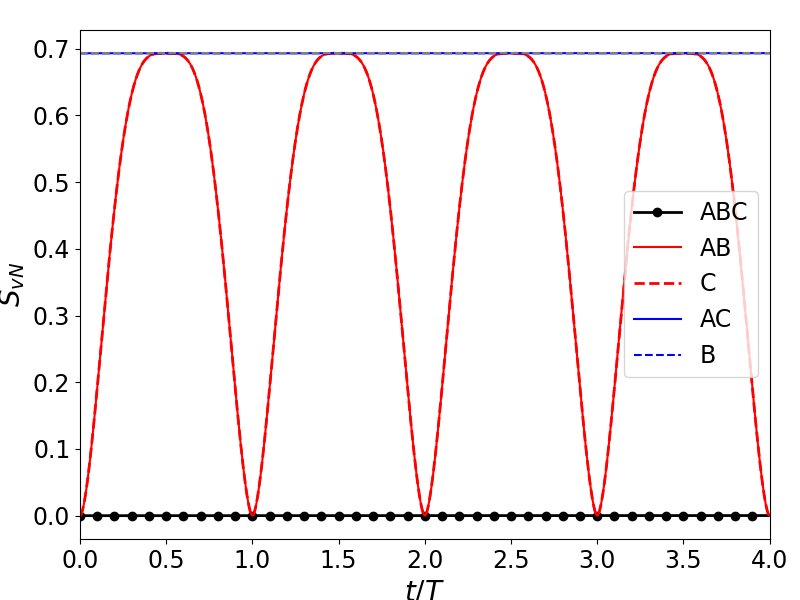
\includegraphics[width=\textwidth]{figuras/ch4/d eg0+ din svn d=0.png}
        \caption{}
        \label{fig4:dinamica svn eg0 sim resonante}
    \end{subfigure}
    \caption{(a):Dinámica poblacional para el caso resonante $\Delta=0$ con el estado inicial entrelazado $\ket{\psi_0}=\frac{1}{\sqrt{2}}(\ket{eg0} + \ket{ge0})$. (b):Entropía de von Neuman del sistema total (negro con puntos), y de diferentes subsistemas. En rojo se muestra la entropía del sistema habiendo trazado parcialmente sobre la cavidad, y en azul habiendo trazado parcialmente sobre el átomo B.}
    \label{fig4:dinamica eg0 sim resonante}
\end{figure}

En la figura \ref{fig4:dinamica pob eg0 sim resonante} se muestran las poblaciones y las coherencias correspondientes a la condición inicial $\ket{\psi_0}=\frac{1}{\sqrt{2}}(\ket{eg0} + \ket{ge0})$ en el caso resonante, y en la figura \ref{fig4:dinamica svn eg0 sim resonante} se muestra la entropía de Von Neuman, en función del tiempo $t/T$ con $T=2 \pi /\Omega(n,j)$  . La entropía de von Neuman es una cantidad que está definida según:
\begin{equation}\label{ec4:entropia von neuman}
    S=-\Tr(\rho \ln \rho)=-\sum_j \lambda_j \ln \lambda_j,
\end{equation}
donde $\rho$ es la matriz densidad del sistema, y $\lambda_j$ son los autovalores de la matriz densidad. La entropía de Von Neuman sirve para determinar si un estado es puro o mixto, ya que $S(\rho)=0$ representa un estado puro, y $S(\rho)=\ln(d)$ representa un estado máximamente mixto, donde $d$ es la dimensión del espacio de Hilbert.
Vemos como el estado $\ket{ge0}$ no evoluciona, ya que en este caso, el átomo B contiene la única excitación y está aislado. Pero la otra parte, si evoluciona. La presencia de las mismas oscilaciones coherentes entre los estados $\ket{eg0}$ y $\ket{gg1}$ es evidente. La diferencia principal es que el estado de los subsistemas es mixto. Esto se observa claramente en el gráfico de la entropía, pero también se puede deducir este comportamiento desde la figura \ref{fig4:dinamica pob eg0 sim resonante}, ya que a $t/T=0.5$, tenemos el estado $\ket{\psi(T/2)}=\ket{g}_A\otimes\frac{1}{\sqrt{2}}(\ket{e_B0_C}+\ket{g_B1_C})$, que es separable solo en el átomo A, y los otros dos están totalmente entrelazados, y por lo tanto, al tomar traza parcial tal que el átomo B y la cavidad estén separadas, este estado es máximamente mixto. Vemos como el entrelazamiento entre la cavidad y el átomo B, que están totalmente aislados, evoluciona indirectamente por medio del átomo A, y paradójicamente, éste queda desentrelazado del sistema para tiempos $t=(k-1/2)T\; ; \; k \in \mathbb{N}$. En este punto notamos algo muy importante, y es que la entropía de von Neuman sólo sirve para estados puros. Cuando $t=0$, la entropía del subsistema AB es 0, porque es un estado puro, y está máximamente entrelazado. Pero al evolucionar, el subsistema AB se hace mixto, y como se observa en la línea azul, la entropía del átomo B es siempre $\log 2$, que según la interpretación de la entropía de von Neuman es que está siempre máximamente entrelazado. Este no es al caso, y la descripción falla porque el estado AB no es puro.

\begin{figure}[h]
    \begin{minipage}[c]{0.67\textwidth}
        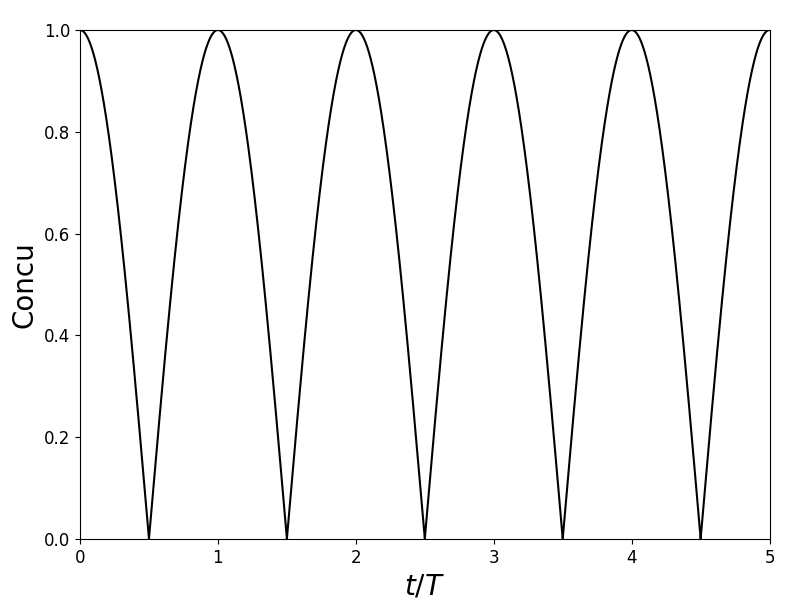
\includegraphics[width=\textwidth]{figuras/ch4/d eg0+ concu d=0.png}
    \end{minipage}\hfill
    \begin{minipage}[c]{0.3\textwidth}
\caption{Concurrencia en el caso resonante para estado inicial $\frac{1}{\sqrt{2}}(\ket{eg0}+\ket{ge0})$} 
    \label{fig4:concu eg0 sim}
  \end{minipage}
\end{figure}

Entonces, ya que el entrelazamiento es un recurso muy importante y va a ser objeto de estudio, es necesario introducir una medida de entrelazamiento más general. Si bien la entropía de Von Neuman es útil en el caso de estados puros, cuando se tienen estados mixtos como mencionamos más arriba, o en el caso de tener un sistema abierto, esta medida ya no sirve. Una de las medidas más utilizadas y con mayor aplicación es el \textit{Entanglement of Formation} ($E_F$) \cite{Plenio2006}, que coincide con la entropía de von Neuman para estados puros, y sirve para estados mixtos. La $E_F$ está definida como
\begin{equation}
    E_F(\rho)=\text{inf}\left( \sum_i p_i E(\ketbra{\psi_i}{\psi_i}) : \rho = \sum_i p_i\ketbra{\psi_i}{\psi_i}\right).
    \label{ec4:entanglement}
\end{equation}
Esta medida representa el entrelazamiento promedio mínimo entre todas las posibles descomposiciones puras de $\rho$, donde $E(\ketbra{\psi_i}{\psi_i})=S(\tr_B{\ketbra{\psi_i}{\psi_i}})$ es la entropía de von Neuman, que es la medida que se utiliza para estados puros. Esta definición es general, pero en el caso presente, donde se estudia el entrelazamiento entre dos sistemas de dos niveles, como lo son los átomos A y B, existe una simplificación muy útil. Esta medida es la concurrencia, y está definida como
\begin{equation}
    C(\rho)=\text{max}\{0,\lambda_1-\lambda_2-\lambda_3-\lambda_4\},
    \label{ec4:concurrencia}
\end{equation}
donde los $\lambda_i$ son las raíces de los autovalores, en orden decreciente, de la matriz \newline $\rho(\sigma_y\otimes\sigma_y)\rho^*(\sigma_y\otimes\sigma_y)$, donde $\rho^*$ es el conjugado (sin transponer) de $\rho$. La concurrencia y la entropía de formación $E_F$ están relacionadas, y la concurrencia obtiene su interpretación a través de ella. Un estado máximamente entrelazado tiene $C(\rho)=1$ y un estado separable $C(\rho)=0$. 


En la figura \ref{fig4:concu eg0 sim} se observa la concurrencia entre los átomos AB, para el caso estudiado anteriormente. Como era de esperar, a $t=0$ el estado es máximamente entrelazado, y luego el entrelazamiento se pierde a $t=T/2$, donde el átomo B está entrelazado con la cavidad. 

\subsection{Interacción átomo-átomo}

El siguiente paso es analizar el rol de las interacciones entre los átomos, aún manteniendo el apantallamiento $\alpha=0$. Para ésto, se siguen utilizando las mismas condiciones iniciales y el átomo B seguirá sin interactuar con la cavidad, pero ahora se considera que la interacción entre átomos, definida por los parámetros $k$ y $J$, será distinta de cero. Para comenzar, en la figura \ref{fig4:k eg0 abc} se observa la evolución temporal para el estado inicial $\ket{\psi_0}=\ket{eg0}$, con $\Delta = 0$, $J=0$ pero $k=0.1g$. Recordar que $k$ es la intensidad de la interacción $\sigma^{(1)}_+\sigma^{(2)}_-+\text{c.c.}$ (ver Ec. (\ref{ec4:H})).

\begin{figure}[h]
    \begin{minipage}[c]{0.67\textwidth}
        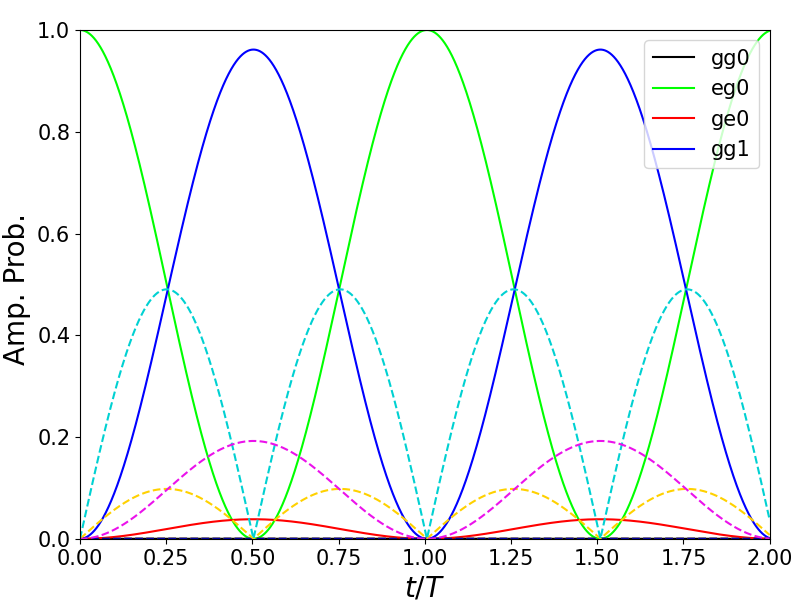
\includegraphics[width=\textwidth]{figuras/ch4/k eg0 ABC.png}
    \end{minipage}\hfill
    \begin{minipage}[c]{0.3\textwidth}
    \caption{Dinámica poblacional para la condición inicial $\ket{\psi_0}=\ket{eg0}$, para los parámetros $\Delta=0$, $J=0$ y $k=0.1g$. Las líneas solidas se corresponden con las poblaciones de la matriz densidad total del sistema; en azul la probabilidad de encontrar al estado en el estado $\ket{gg1}$, en verde en $\ket{eg0}$, en rojo $\ket{ge0}$, y en negro $\ket{gg0}$. Las líneas rayadas son las coherencias entre estas poblaciones, la violeta entre $\ket{gg1}$ y $\ket{ge0}$, la celeste entre $\ket{eg0}$ y $\ket{gg1}$ y la amarilla entre $\ket{eg0}$ y $\ket{gg1}$.
         } \label{fig4:k eg0 abc}
  \end{minipage}
\end{figure}
Lo que sucede es que la excitación está inicialmente en el átomo A, y como siempre, se observan oscilaciones entre los estados $\ket{eg0}$ y $\ket{gg1}$, la diferencia es que al haber interacciones entre los átomos, ahora la excitación inicial que está en el átomo A, sufre dos procesos diferentes, primero la oscilación, y además, la interacción con el átomo B. Al tener la excitación el átomo A, una parte de ésta se va hacia la cavidad, y la otra hacia el átomo B, excitándolo parcialmente. La amplitud de la oscilación depende de la intensidad de la interacción $k$. Mediante la curva roja, se contempla que su pendiente crece mientras que la probabilidad de $\ket{eg0}$ es mayor a la de $\ket{gg1}$. Cuando las probabilidades cambian, la amplitud crece, pero de manera desacelerada, hasta que la probabilidad del estado $\ket{eg0}$ es nula. En ese momento, ya no hay excitación que pasar del átomo A al B, y el proceso se revierte. Antes de analizar el entrelazamiento entre los átomos, se observa en la figura \ref{fig4:k eg0 sim abc} la dinámica para los mismos parámetros, pero para la condición inicial entrelazada $\ket{\psi_0}=\frac{1}{\sqrt{2}}(\ket{eg0}+\ket{ge0})$:
\begin{figure}[h]
    \begin{minipage}[c]{0.67\textwidth}
        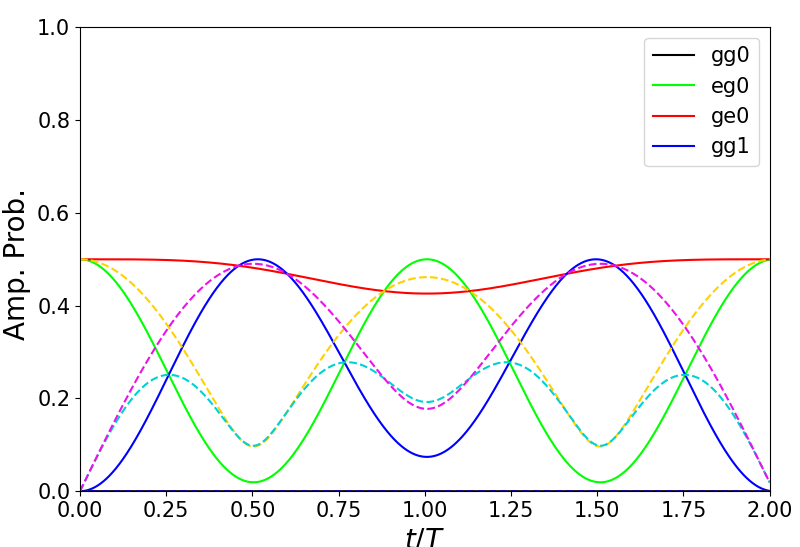
\includegraphics[width=\textwidth]{figuras/ch4/k eg0+ ABC.png}
    \end{minipage}\hfill
    \begin{minipage}[c]{0.3\textwidth}
    \caption{Dinámica poblacional para la condición inicial $\ket{\psi_0}=\frac{1}{\sqrt{2}}(\ket{eg0}+\ket{ge0})$, para los parámetros $\Delta=0$, $J=0$ y $k=0.1g$. Las coherencias y poblaciones tienen los mismos colores que la figura anterior \ref{fig4:k eg0 abc}}
    \label{fig4:k eg0 sim abc}
  \end{minipage}
\end{figure}
La dinámica en este caso presenta oscilaciones en la población de $\ket{ge0}$ con un periodo dos veces más grande. Esto se debe a una \textit{pelea} entre los estados $\ket{eg0}$ y $\ket{ge0}$, ya que tienen las excitaciones en diferentes átomos. Inicialmente, como los estados están entrelazados, no está bien definido en cuál de los dos átomos está la excitación, entonces la interacción $k$ se anula y la curva tiene pendiente 0. Entonces la dinámica inicial es igual que para $k=0$ y comienza a oscilar. Al decrecer la curva verde, la probabilidad de encontrar la excitación en el átomo B es mayor que la del átomo A, entonces el átomo B comienza a perder esta excitación y se la da lentamente al átomo A, y por lo tanto la oscilación del estado $\ket{eg0}$ no llega a tener amplitud nula en $t/T=0.5$. Luego, la evolución sigue su curso oscilante, y al llegar a $t=T$, la probabilidad de encontrar la excitación en el átomo A es mayor que en el átomo B, y por lo tanto comienza a revertirse la situación, hasta completar el ciclo en $t=2T$. 

El entrelazamiento entre los átomos se analiza utilizando la concurrencia, como se muestra en la figura \ref{fig4:concu k}, donde \ref{fig4:concu k eg0} muestra la condición inicial separable $\ket{eg0}$, y \ref{fig4:concu k eg0 sim} el entrelazamiento para la condición inicial entrelazada $\frac{1}{\sqrt{2}}(\ket{eg0}+\ket{ge0})$. 
\begin{figure}[h]
    \centering
    \begin{subfigure}{0.49\textwidth}
        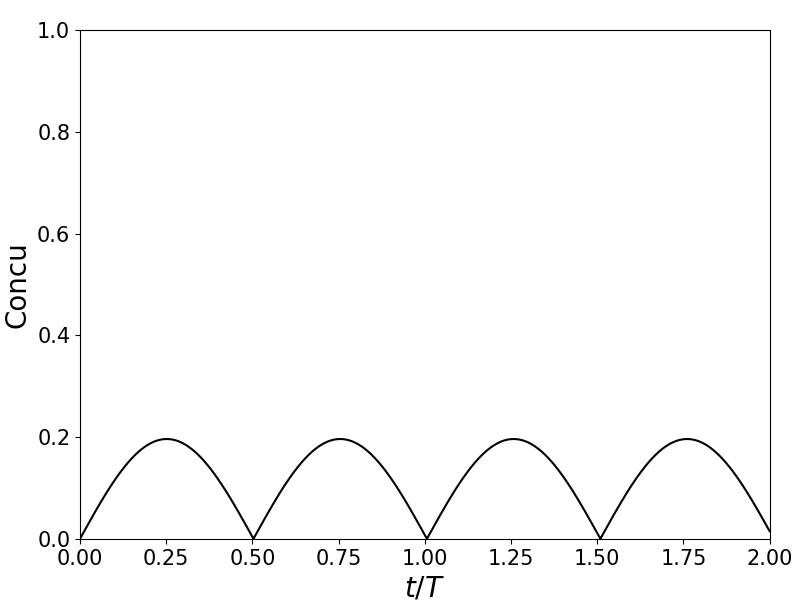
\includegraphics[width=\textwidth]{figuras/ch4/k eg0 concu.png}
        \caption{}
        \label{fig4:concu k eg0}
    \end{subfigure}
    \hfill
    \begin{subfigure}{0.49\textwidth}
        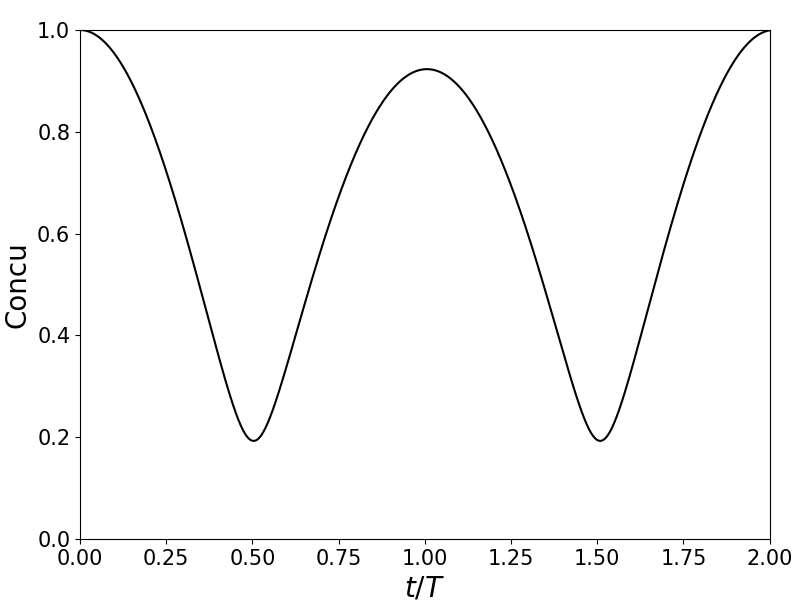
\includegraphics[width=\textwidth]{figuras/ch4/k eg0+ concu.png}
        \caption{}
        \label{fig4:concu k eg0 sim}
    \end{subfigure}
    \caption{Dinámica de entrelazamiento para $\Delta=0$, $J=0$ y $k=0.1g$ para el estado inicial (a)$\ket{eg0}$ y (b)$\frac{1}{\sqrt{2}}(\ket{eg0}+\ket{ge0})$}
    \label{fig4:concu k}
\end{figure}

Ahora se analiza la interacción tipo Ising, para eso se utilizan parámetros $k=0$ y $J\neq 0$. En la figura \ref{fig4:j alpha0} se observa que, si bien la dinámica es similar, los átomos no se entrelazan.

\begin{figure}[H]
    \centering
    \begin{subfigure}{0.49\textwidth}
        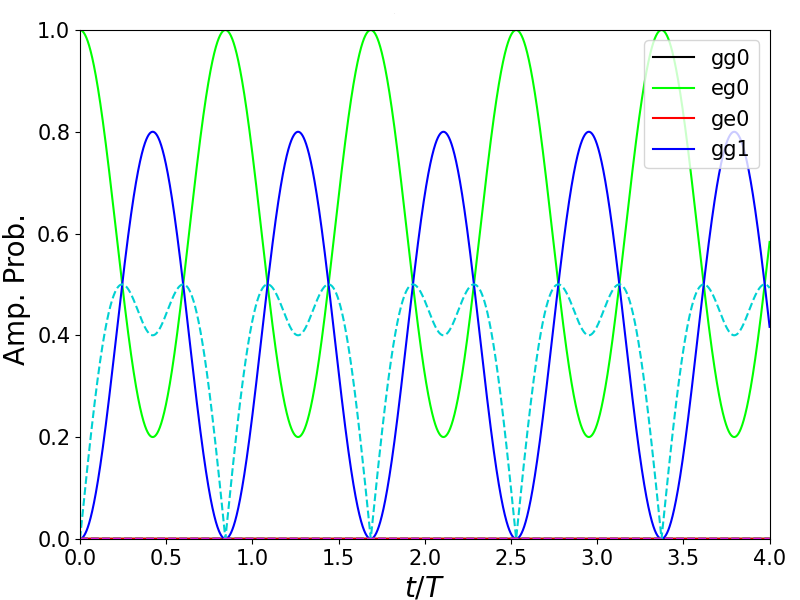
\includegraphics[width=\textwidth]{figuras/ch4/j eg0 abc.png}
        \caption{}
        \label{fig4:pob j eg0}
    \end{subfigure}
    \hfill
    \begin{subfigure}{0.49\textwidth}
        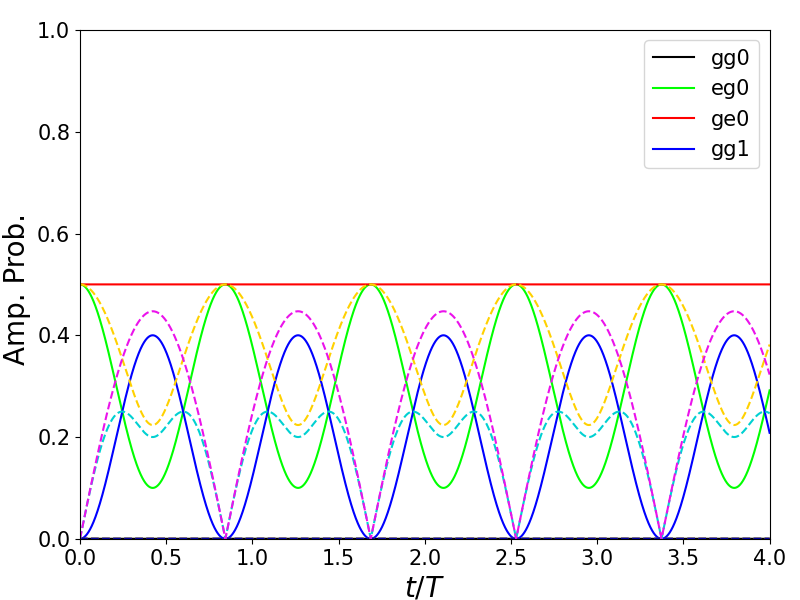
\includegraphics[width=\textwidth]{figuras/ch4/j eg0+ge0 abc.png}
        \caption{}
        \label{fig4:pob j eg0 sim}
    \end{subfigure}
    \vfill
    \begin{subfigure}{0.49\textwidth}
        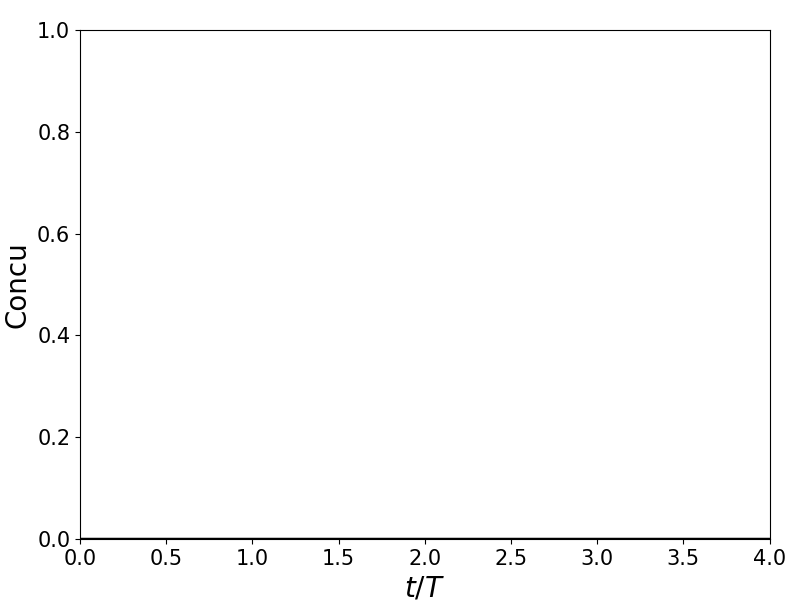
\includegraphics[width=\textwidth]{figuras/ch4/j eg0 concu.png}
        \caption{}
        \label{fig4:pob j eg0}
    \end{subfigure}
    \hfill
    \begin{subfigure}{0.49\textwidth}
        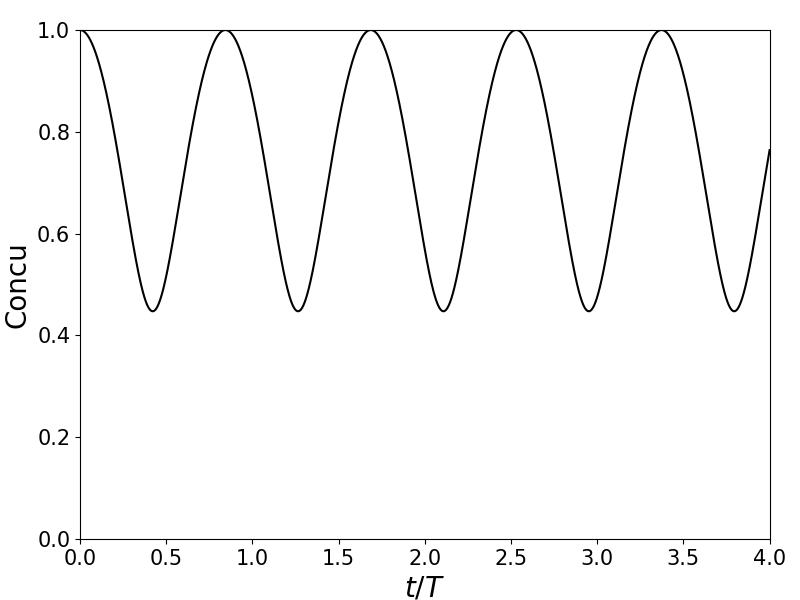
\includegraphics[width=\textwidth]{figuras/ch4/j eg0+ge0 concu.png}
        \caption{}
        \label{fig4:pob j eg0 sim}
    \end{subfigure}
    \caption{Dinámica con parámetros $\Delta=0$, $J=0.5g$ y $k=0$. En (a) las poblaciones y (c) la concurrencia del estado inicial es $\ket{eg0}$, y en (b) las poblaciones, y (d) la concurrencia del estado inicial $\frac{1}{\sqrt{2}}(\ket{eg0}+\ket{ge0})$.}
    \label{fig4:j alpha0}
\end{figure}
La diferencia principal entre la interacción tipo Isign ($J\sigma_z^{(1)}\sigma_z^{(2)}$) y la dipolar ($k\sigma_+^{(1)}\sigma_-^{(2)}+\text{c.c.}$), es que el segundo parece entrelazar los átomos, ya que en el primer caso, el efecto es separar los niveles de energía, pero en el segundo no solo eso, sino que también pasa excitaciones de un átomo al otro. Si bien esto sirve para entender intuitivamente el efecto, el problema de este análisis es que se asumen cosas no físicas mediante el apantallamiento y la asimetría que se impone entre los dos átomos. Ya que en el Hamiltoniano del sistema sin apantallamiento (Ec. (\ref{ec4:H})), donde se utiliza la base con estados simétricos y antisimétricos (Ec. (\ref{ec4:base})), el efecto de ambos parámetros debería ser el mismo, ya que solo aparecen en la diagonal principal. Si bien la interacción $J$ actúa sobre todos los estados, y el $k$ solamente solo sobre los $\frac{1}{\sqrt{2}}(\ket{egn}\pm \ket{gen})$, su principal función es separar las energías de los estados de la base.
Entonces será necesario retomar este análisis sin apantallamiento y con la base adecuada de la Ec.(\ref{ec4:base}).

\subsection{Medio Kerr}
\label{sec4:medio kerr}

En esta sección estudiamos el efecto del medio Kerr. Para ésto, se apagan las interacciones interatómicas $k=J=0$, y se modifica la no linealidad del medio a través del parámetro $\chi$. 
\begin{figure}[h]
    \centering
    \begin{subfigure}{0.49\textwidth}
        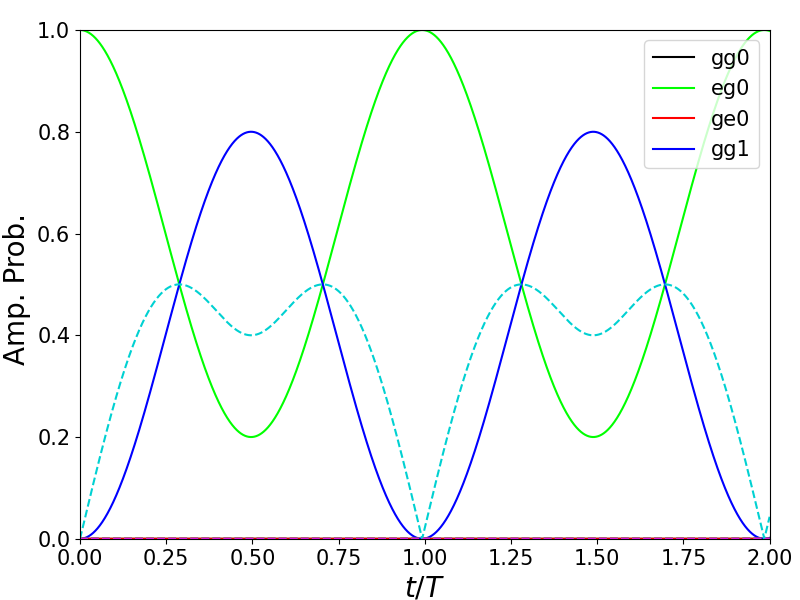
\includegraphics[width=\textwidth]{figuras/ch4/x eg0 abc.png}
        \caption{}
        \label{fig4:pob x eg0}
    \end{subfigure}
    \hfill
    \begin{subfigure}{0.49\textwidth}
        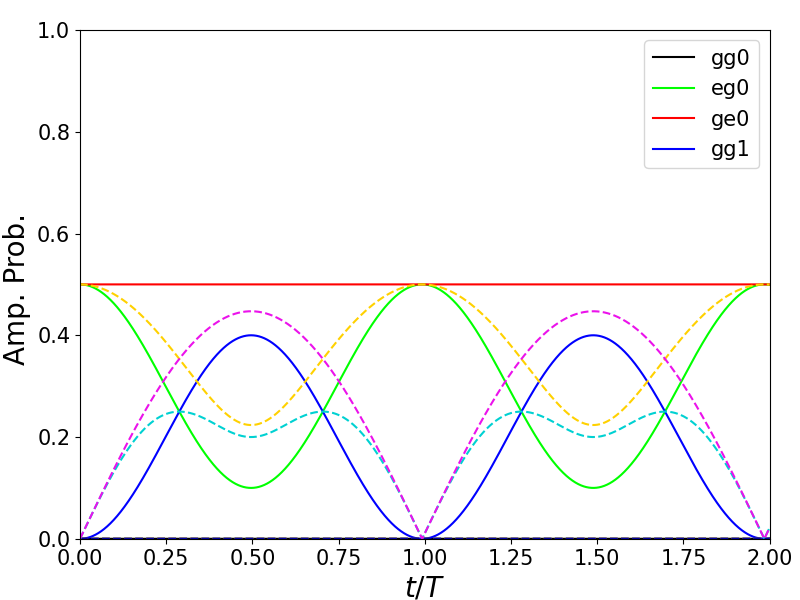
\includegraphics[width=\textwidth]{figuras/ch4/x eg0+ abc.png}
        \caption{}
        \label{fig4:pob x eg0 sim}
    \end{subfigure}
    \caption{Dinámica de poblaciones para $x=g$ con el estado inicial (a) $\ket{eg0}$ y (b) $\frac{1}{\sqrt{2}}(\ket{eg0}+\ket{ge0})$}
    \label{fig4:pob x}
\end{figure}

Al igual que en el caso de 1 átomo, se puede observar en las Ec. (\ref{ec4:autoenergias}) y Ec. (\ref{ec4:parametros solucion}) que la frecuencia depende del medio. En la figura \ref{fig4:pob x} el tiempo está normalizado con la frecuencia, entonces no se nota el cambio. Pero lo que es necesario analizar, es cómo las oscilaciones no son totalmente coherentes, en el sentido de que la amplitud de probabilidad no es 1, como en el caso de $\chi=0$. Esto se debe a que el aumento de $\chi$ hace que las energías de ambos estados se separen, y por lo tanto las transiciones entre los estados sean menos probables. Este comportamiento también se observa si el estado inicial se toma como $\ket{gg1}$. Es lógico estudiar el entrelazamiento en este caso. En la figura \ref{fig4:concu x} se muestran las concurrencias para ambas condiciones iniciales. Es interesante comparar la figura \ref{fig4:concu x eg0 sim} con la figura cuando $\chi=0$, para esta misma condición inicial, representada en la figura \ref{fig4:concu eg0 sim}. La diferencia se encuentra en la amplitud de oscilación. Si bien ambos comienzan a $t=0$ en $C=1$, cuando el medio es lineal ($\chi=0$) la concurrencia oscila hasta llegar a su mínimo en $C=0$, en cambio cuando $\chi=g$ las oscilaciones llegan solamente hasta $C=0.4$ aproximadamente. En principio, se puede pensar que el medio no lineal rompe con el entrelazamiento del sistema. Pero como se ve al comparar estas figuras, la interpretación correcta es que el medio no hace más que ralentizar el comportamiento preexistente de la cavidad, ya que en este caso, no destruye el entrelazamiento, sino que lo conserva por virtud de haber ralentizado el proceso: las amplitudes de oscilación entre los dos estados dinámicos son menores.
\begin{figure}[h]
    \centering
    \begin{subfigure}{0.49\textwidth}
        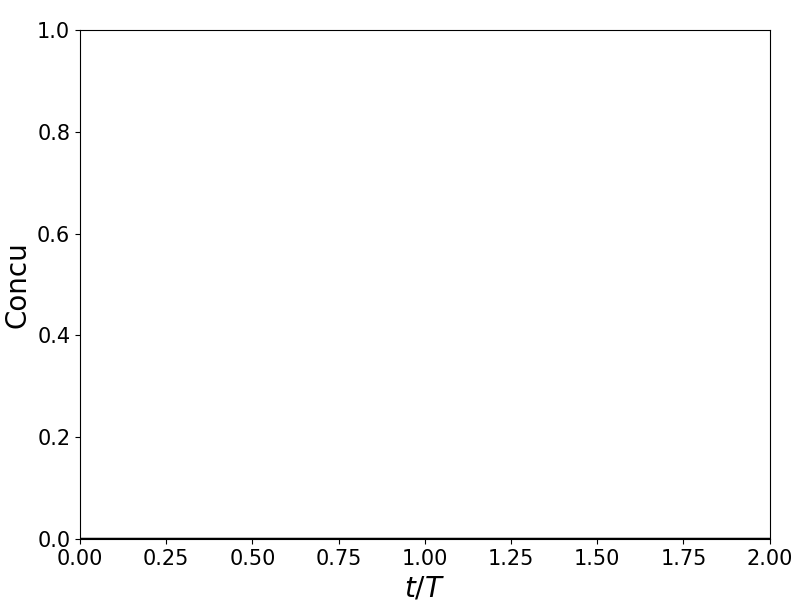
\includegraphics[width=\textwidth]{figuras/ch4/x eg0 concu.png}
        \caption{}
        \label{fig4:concu x eg0}
    \end{subfigure}
    \hfill
    \begin{subfigure}{0.49\textwidth}
        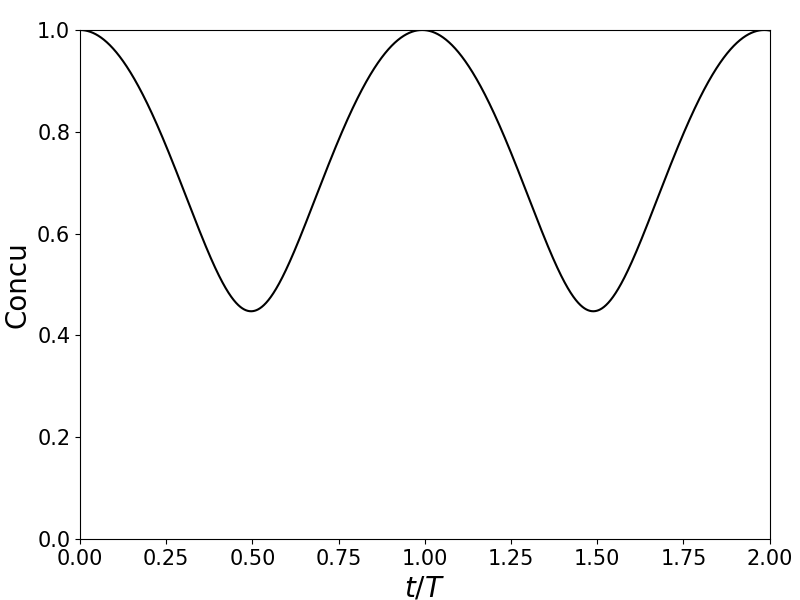
\includegraphics[width=\textwidth]{figuras/ch4/x eg0+ concu.png}
        \caption{}
        \label{fig4:concu x eg0 sim}
    \end{subfigure}
    \caption{Dinámica de entrelazamiento para $x=g$ para estados iniciales (a) $\ket{eg0}$ y (b) $\frac{1}{\sqrt{2}}(\ket{eg0}+\ket{ge0})$}
    \label{fig4:concu x}
\end{figure}
También se puede recuperar el comportamiento visto en el modelo de 1 átomo, que el medio Kerr no es más que un desplazamiento lateral en las frecuencias, además de modificar las amplitudes. Para esto se realiza otra evolución para $\chi=\Delta=\frac{g}{2}$, y se compara con el caso en que $\chi=\Delta=0$
\begin{figure}[h]
    \centering
    \begin{subfigure}{0.49\textwidth}
        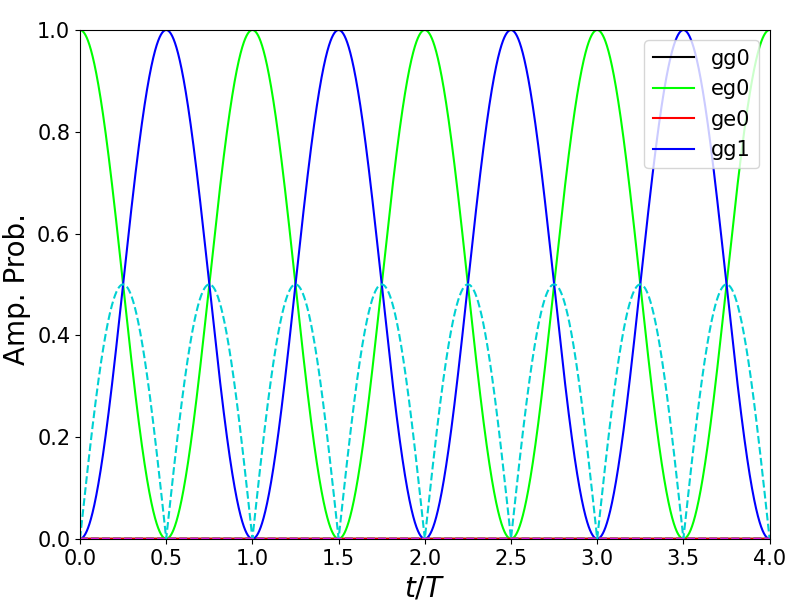
\includegraphics[width=\textwidth]{figuras/ch4/d=x=0 eg0 abc.png}
        \caption{}
        \label{fig4:comparacion kerr pob 1}
    \end{subfigure}
    \hfill
    \begin{subfigure}{0.49\textwidth}
        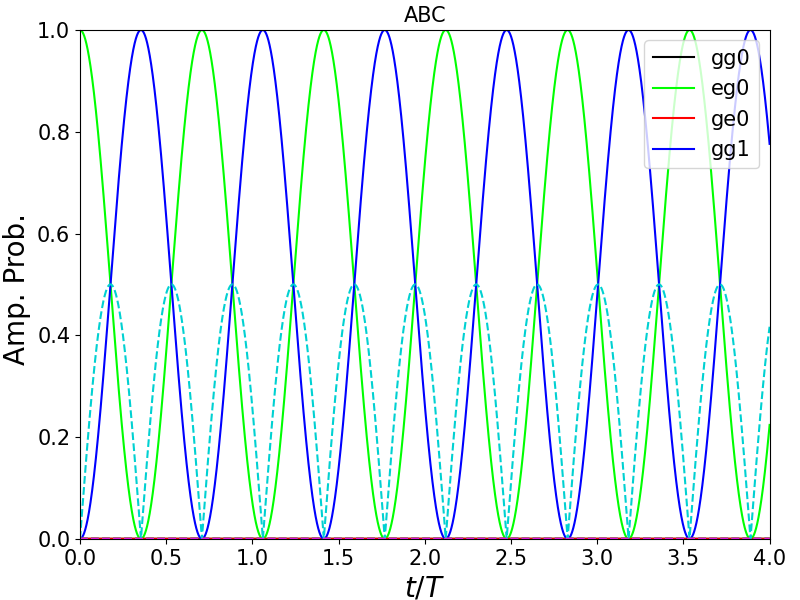
\includegraphics[width=\textwidth]{figuras/ch4/d=x=0.5 eg0 abc.png}
        \caption{}
        \label{fig4:comparacion ker pob 2}
    \end{subfigure}
    \caption{Dinámica de poblaciones para estado inicial $\ket{eg0}$ con (a) $\Delta=\chi=0$ y (b) $\Delta=\chi=0.5g$}
    \label{fig4:comparacion d vs x}
\end{figure}
Se observa cómo se anula el efecto del medio, y la dinámica es la misma pero con un cambio en la frecuencia. Al igual que antes, aumenta el tiempo característico del sistema y por lo tanto la frecuencia es mayor en el segundo caso.

\subsection{Batidos}

Al complejizar el problema, la dinámica comienza a presentar batidos entre las amplitudes de probabilidad de las poblaciones y en las coherencias, comportamiento que se atribuye a la modulación de dos procesos simultáneos. Por ejemplo, en la evolución temporal con $\chi\neq0$ y $k\neq0$, el primero disminuye la amplitud de oscilación de los estados con mayor cantidad de fotones en la cavidad, que dentro del subespacio $N$ la jerarquía del medio sera favorecer a los estados $\ket{eg,N-1}$ y $\ket{ge,N-1}$ por sobre el $\ket{ggN}$. Por el contrario, se observó que en esta situación, el término de interacción entre los átomos disminuye la amplitud del estado $\ket{ggN}$ como se vio en la sección anterior. Por lo tanto, si dos procesos están en juego y sus efectos son similares, es esperable que se observen oscilaciones moduladas. No vale la pena mostrar la dinámica de las poblaciones, porque no se pueden sacar conclusiones muy importantes, pero sí podemos observar la trayectoria en la esfera de Bloch, para dar una idea de la complejidad de la evolución.
\begin{figure}[h]
    \centering
    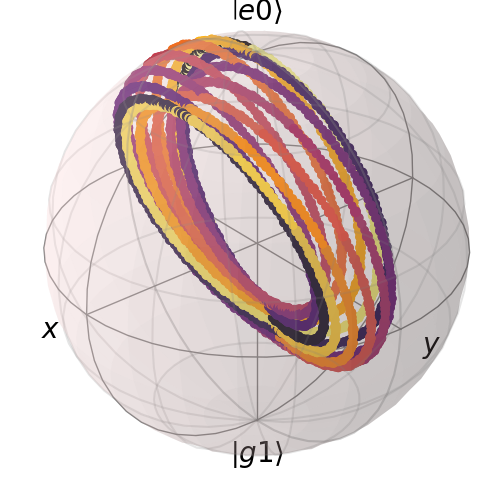
\includegraphics[width=0.5\linewidth]{figuras/ch4/eg0 bloch AC a=0 d=0.0 x=0.5 k=0.5 J=0.0 gamma=0.0 p=0.0.png}
    \caption{Trayectoria en la esfera de Bloch para el estado inicial $\ket{eg0}$, trazando parcialmente sobre el átomo B, y los parámetros utilizados son $\Delta=0$,$\chi=0.5g$,$k=0.5g$ y $J=0$.}
    \label{fig4:eg0 bloch batidos}
\end{figure}
En la figura \ref{fig4:eg0 bloch batidos} se representa la trayectoria en el espacio de estados cuyo estado inicial es $\ket{eg0}$, habiendo trazado parcialmente sobre el átomo B que está apantallado. Es evidente por la curva descrita en la esfera de Bloch, que la dinámica es complicada y los análisis poblacionales carecen de sentido, ya que se pierde la periodicidad. En este gráfico, el color representa el tiempo comenzando por el color negro, y aclarándose hasta llegar a $t=7T$, representado por el color amarillo. 
\section{Dinámica sin apantallamiento}
\label{sec4:dinamica sin apantallamiento}

Al sacar el apantallamiento, es necesario utilizar la base de la Ec. (\ref{ec4:base}), ya que los átomos son indistinguibles y esta base es más apropiada. Además, el Hamiltoniano desacopla los estados antisimétricos, facilitando la solución. Resulta de interés estudiar el entrelazamiento entre los átomos, y su dependencia con los parámetros. 

\subsection{Dinámica con disipación}
Para modelar la dinámica disipativa se utiliza nuevamente el formalismo de la ecuación de Lindblad, donde los operadores de colapso ahora deben tener en cuenta a ambos átomos por igual. Se consideran los procesos de pérdidas al igual que en el caso de un átomo como la pérdida de fotones por las imperfecciones de la cavidad, y el bombeo incoherente de los átomos. La ecuación maestra ahora tiene los operadores

\begin{align}
    L_\gamma&=\sqrt{\gamma}\hat a, \\
    L_p &=\sqrt{p}(\hat\sigma_+^{(1)}+\hat\sigma_+^{(2)}).  
\end{align}
Explícitamente la ecuación de Lindblad es
\begin{equation}
\begin{aligned}
    \dot \rho(t) &= -i\bigg[\rho(t),\chi \hat n^2+\frac{ \Delta}{2}(\hat\sigma_Z^{(1)}+\hat\sigma_Z^{(2)})   
     +  g(\hat\sigma_+^{(1)}\hat a f(\hat n)+\hat\sigma_-^{(1)}f(\hat n) \hat a^\dagger + \hat\sigma_+^{(2)}\hat a f(\hat n) \\ &+\hat\sigma_-^{(2)}f(\hat n) \hat a^\dagger) + 2 \kappa (\hat \sigma_-^{(1)}\hat \sigma_+^{(2)}+\hat \sigma_+^{(1)}\hat \sigma_-^{(2)}) +  J \hat \sigma_Z^{(1)}\hat \sigma_Z^{(2)}\bigg] \\ &+ \gamma\left(\hat a\rho(t) \hat a^\dagger -\frac{1}{2}\left\{  \hat a^\dagger \hat a ,\rho(t) \right\} \right) + p\left(\hat\sigma_+\rho(t)\hat\sigma_--\frac{1}{2}\left\{\hat\sigma_-\hat\sigma_+,\rho(t)\right\}\right),
     %-\frac{1}{2}\rho(t)\hat\sigma_-\hat\sigma_+\right),
\end{aligned}
\end{equation}
donde $\hat\sigma_\pm=(\hat\sigma_\pm^{(1)}+\hat\sigma_\pm^{(2)})$.
Este es un sistema de ecuaciones acopladas, y la necesitad de acudir a métodos numéricos es evidente.

Lo primero que hay que considerar es la dependencia de la dinámica con el régimen de acoplamiento, se espera un comportamiento igual al del caso de un átomo (sección \ref{sec3:regimen acoplamiento}). Recordar que el régimen de acoplamiento fuerte (SC) es el caso en donde la interacción entre cavidad y átomos es mayor a la interacción entre sistema y entorno.
\begin{figure}[h]
    \centering
    \begin{subfigure}{0.7\textwidth}
        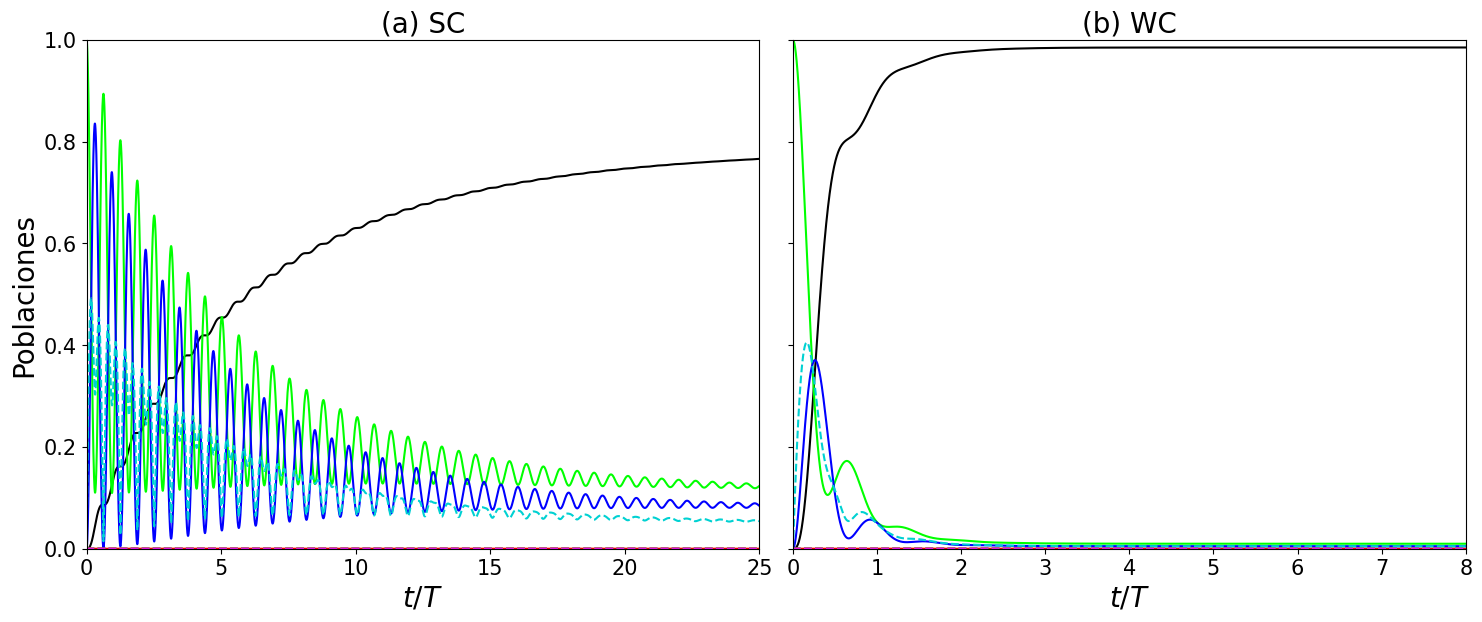
\includegraphics[width=\textwidth]{figuras/ch4/sc vs wc eg0 sim j0.5.png}
        \caption{}
        \label{fig4:acoplamiento eg0 sim}
    \end{subfigure}
    \vfill
    \begin{subfigure}{0.7\textwidth}
        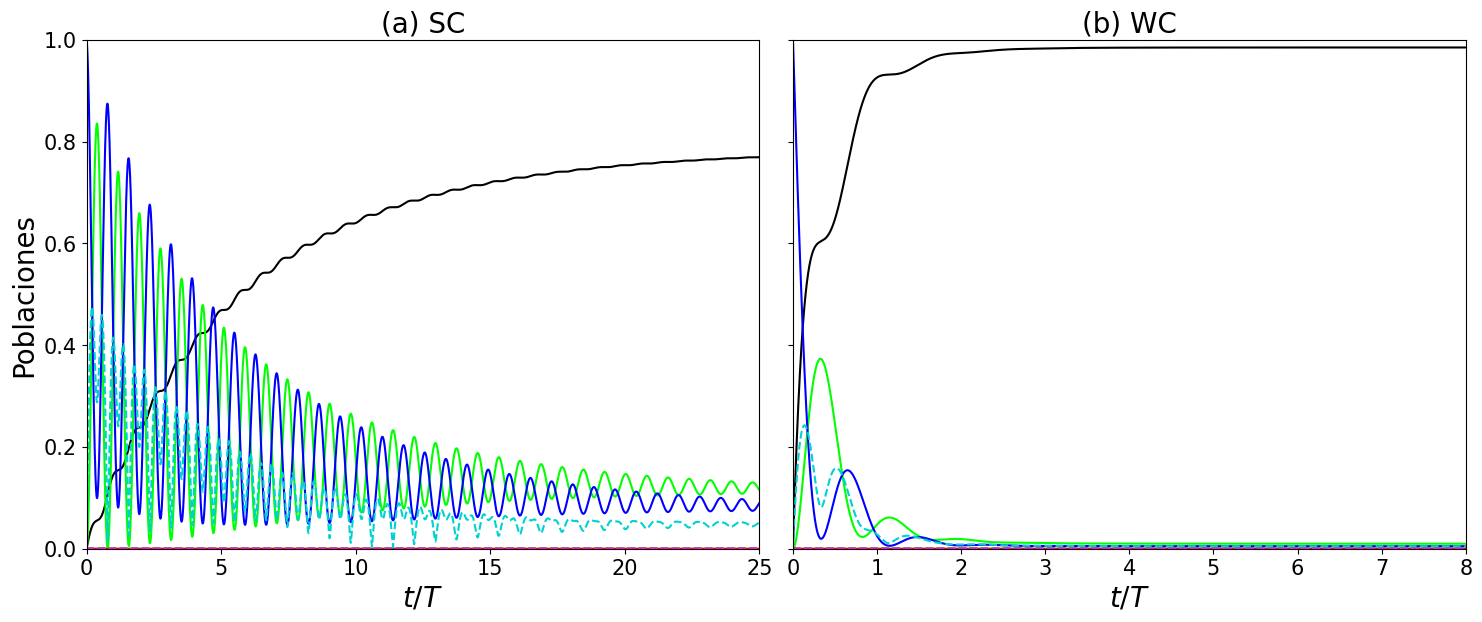
\includegraphics[width=\textwidth]{figuras/ch4/sc vs wc gg1 k=0.5.png}
        \caption{}
        \label{fig4:acoplamiento gg1}
    \end{subfigure}
    \caption{Dependencia de las poblaciones con el régimen de acoplamiento, para $\Delta=J=\chi=0$ y $k=0.5g$, y para dos condiciones iniciales diferentes. (a) $\frac{1}{\sqrt{2}}(\ket{eg0}+\ket{ge0})$, $\Delta=\chi=k=0$, $J=0.5g$; (b) $\ket{gg1}$, $\Delta=\chi=J=0$, $k=0.5g$.}
    \label{fig4:regimen acoplamiento}
\end{figure}
En  la figura \ref{fig4:regimen acoplamiento} se muestran las coherencias y las poblaciones. Como se esperaba, estas tienen el mismo comportamiento que en el caso de 1 átomo. Notablemente, se puede ver el efecto de la interacción entre los átomos. Como las energías se separan inicialmente, las oscilaciones no logran la inversión total de población, solo una inversión parcial, y a tiempos largos la disipación hace que se tenga una mayor probabilidad de encontrar al sistema en el estado $\frac{1}{\sqrt{2}}(\ket{eg0}+\ket{ge0})$ ya que tiene menor energía. Eventualmente alcanza su estado estacionario. Lo que se recupera, ahora que ya no hay apantallamiento, es que ambos tipos de interacción ($J$ y $k$) generan entrelazamiento, consecuentemente la concurrencia para ambas interacciones es oscilante. 

 Nuevamente, nos concentraremos en el régimen SC. Si bien hasta ahora se estudió principalmente estados con una excitación, interesantes por sus implicancias y similitudes al modelo de 1 átomo, considerar estados con mayor cantidad de excitaciones hace a la riqueza del problema. Si solo consideramos $N=1$, el subespacio del problema tiene tres estados, de los cuales uno es el estado antisimétrico $\frac{1}{\sqrt{2}}(\ket{eg0}-\ket{ge0})$ que está desconectado de los otros estados, y por lo tanto efectivamente se tiene un modelo de Jaynes-Cummings de 1 átomo con dos estados dinámicamente relevantes. Si se permiten $N=2$ excitaciones, ahora hay cuatro estados en el subespacio, de los cuales tres son relevantes. Primero veremos cuales son los efectos de las interacciones y la dinámica para estados iniciales en el subespacio de $N=2$. Para mantener el paralelismo, comenzaremos con el estado $\frac{1}{\sqrt{2}}(\ket{eg1}+\ket{ge1})$, pero como se verá, las condiciones iniciales cambian totalmente la dinámica de entrelazamiento del sistema. La enorme cantidad de posibilidades para elegir condiciones iniciales, hace que estudiar todos sea imposible, así que se  concentrarán los esfuerzos en algunos de ellos.
Al tener tres estados dinámicamente relevantes, se tienen tres autoestados con sus respectivas autoenergías, y por lo tanto tres frecuencias que compiten entre sí, y son las tres frecuencias de Rabi del sistema:
\begin{equation}
    \begin{aligned}
        \Omega^{(n)}_{12} &= E^{(n)}_2-E^{(n)}_1 ,\\
        \Omega^{(n)}_{23} &=E^{(n)}_3-E^{(n)}_2, \\
        \Omega^{(n)}_{31} &= E^{(n)}_1-E^{(n)}_3 .        
    \end{aligned}
    \label{ec4:frecuencias de rabi}
\end{equation}
Estas frecuencias se muestran en función del detunning $\Delta$ y para diferentes valores de $\chi$ y de $k-J$ en la figura \ref{fig4:frecuencias de rabi}.
\begin{figure}
    \centering
    \begin{subfigure}{0.49\textwidth}
        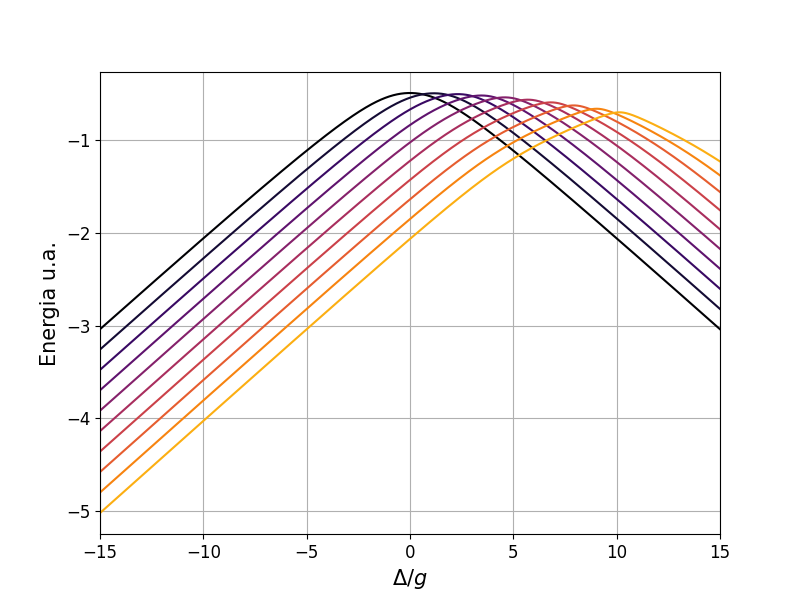
\includegraphics[width=\textwidth]{figuras/ch4/omega12 2d chi.png}
        \caption{}
        \label{fig4:rabi 1 chi}
    \end{subfigure}
    \hfill
    \begin{subfigure}{0.49\textwidth}
        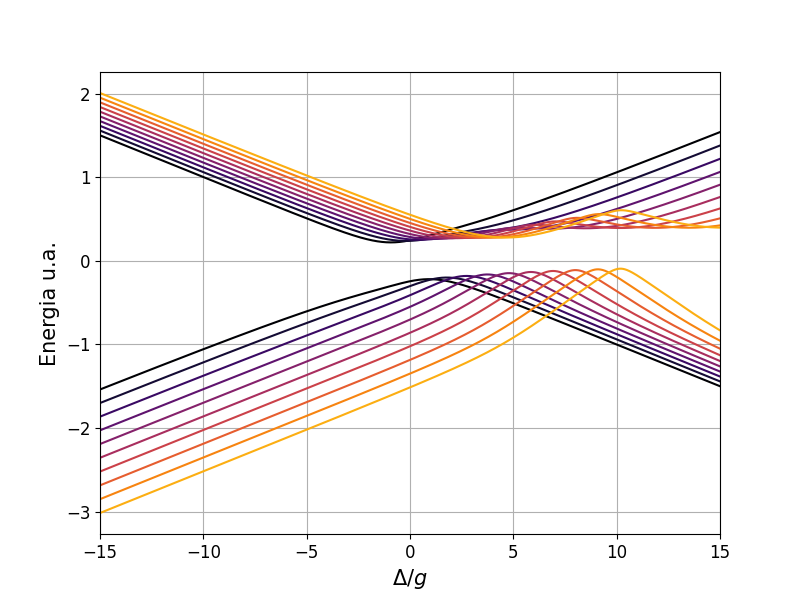
\includegraphics[width=\textwidth]{figuras/ch4/omega23 2d chi.png}
        \caption{}
        \label{fig4:rabi 2 chi}
    \end{subfigure}
    \vfill
    \begin{subfigure}{0.49\textwidth}
        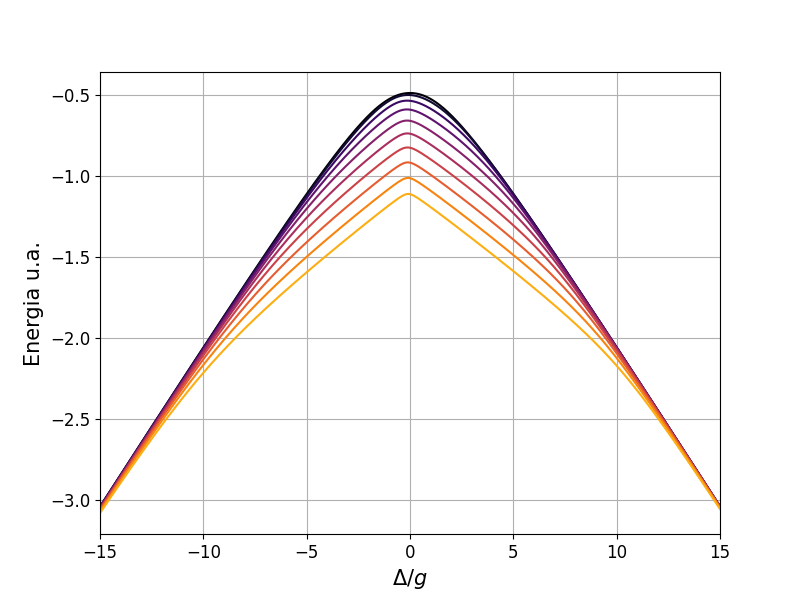
\includegraphics[width=\textwidth]{figuras/ch4/omega12 2d k.png}
        \caption{}
        \label{fig4:rabi 1 k}
    \end{subfigure}
    \hfill
    \begin{subfigure}{0.49\textwidth}
        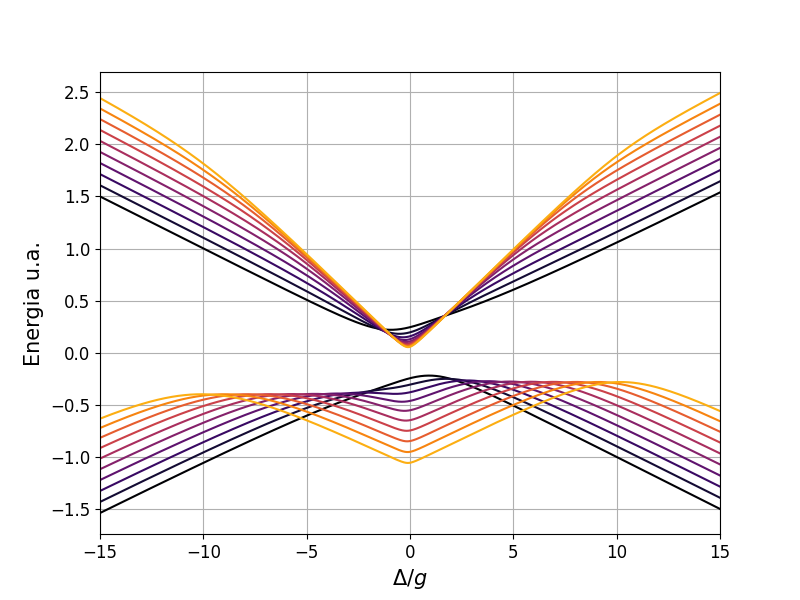
\includegraphics[width=\textwidth]{figuras/ch4/omega23 2d k.png}
        \caption{}
        \label{fig4:rabi 2 k}
    \end{subfigure}
    \caption{Frecuencias de Rabi en función del detunning $\Delta$ para diferentes valores de $\chi$, y $|k-J|$, donde las frecuencias de Rabi son $\Omega^{(2)}_{ij}=E^{(2)}_{j}-E^{(2)}_{i}$. (a) $\Omega_{12}$ con $\chi\in [0,5g]$; (b) $\Omega_{23}$ y $\Omega_{31}$ con $\chi\in [0,5g]$ ;(c) $\Omega_{12}$ con $k-J\in [0,5g]$ ; (d) $\Omega_{23}$ y $\Omega_{31}$ con $k-J\in [0,5g]$}
    \label{fig4:frecuencias de rabi}
\end{figure}


% \begin{figure}
%     \centering
%     \begin{subfigure}{0.3\textwidth}
%         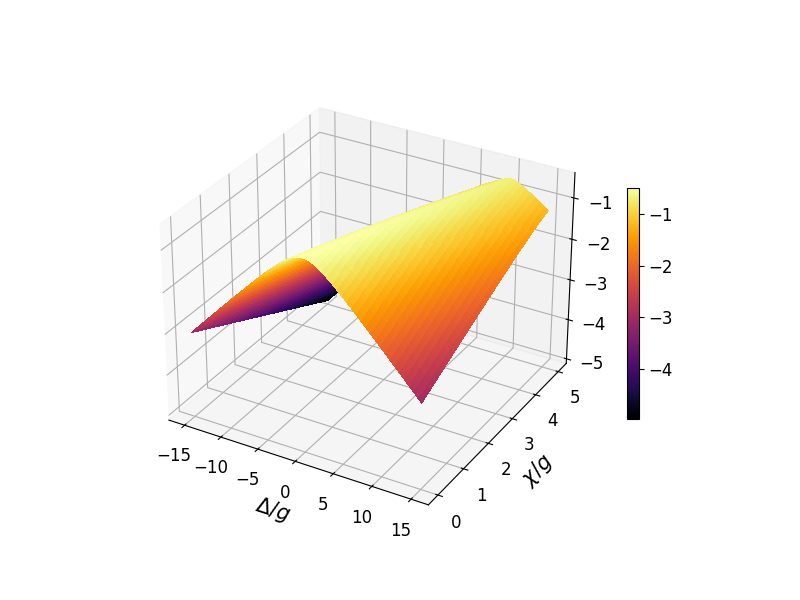
\includegraphics[width=\textwidth]{figuras/ch4/omega12 k=0.png}
%         \caption{}
%         \label{fig4:rabi chi}
%     \end{subfigure}
%     \hfill
%     \begin{subfigure}{0.3\textwidth}
%         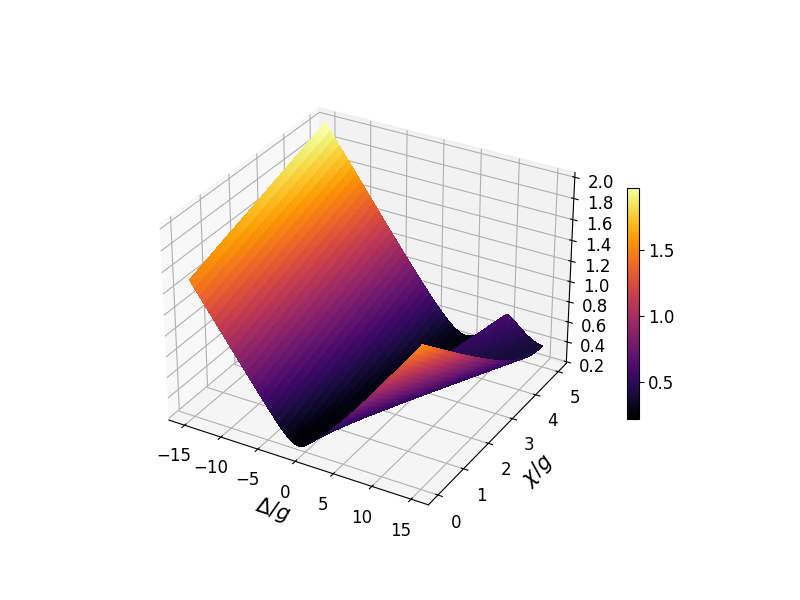
\includegraphics[width=\textwidth]{figuras/ch4/omega23 k=0.png}
%         \caption{}
%         \label{fig4:rabi chi}
%     \end{subfigure}
%     \hfill
%     \begin{subfigure}{0.3\textwidth}
%         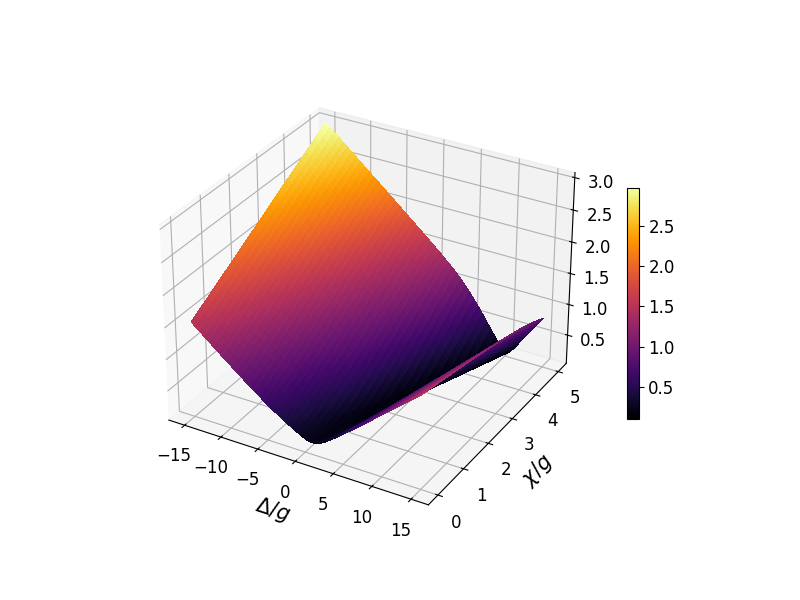
\includegraphics[width=\textwidth]{figuras/ch4/omega31 k=0.png}
%         \caption{}
%         \label{fig4:rabi chi}
%     \end{subfigure}
%     \vfill
%     \begin{subfigure}{0.3\textwidth}
%         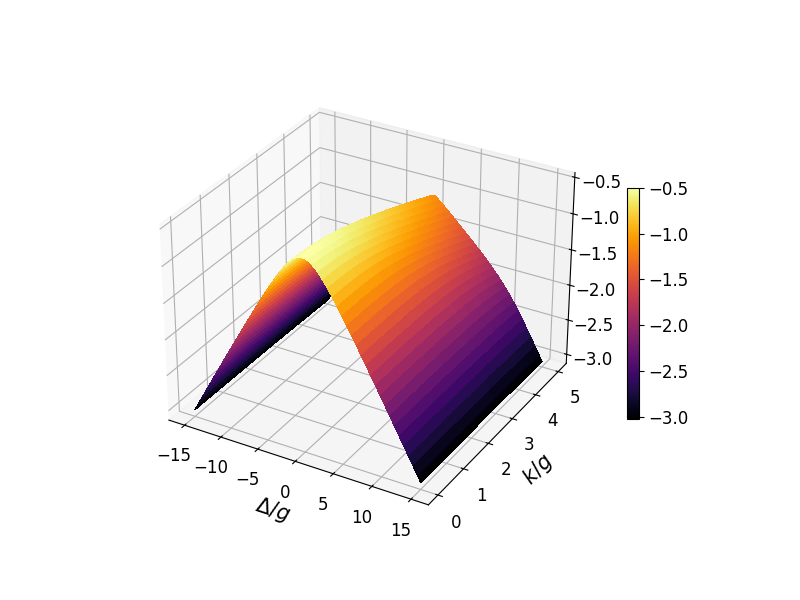
\includegraphics[width=\textwidth]{figuras/ch4/omega12 x=0.png}
%         \caption{}
%         \label{fig4:rabi chi}
%     \end{subfigure}
%     \hfill
%     \begin{subfigure}{0.3\textwidth}
%         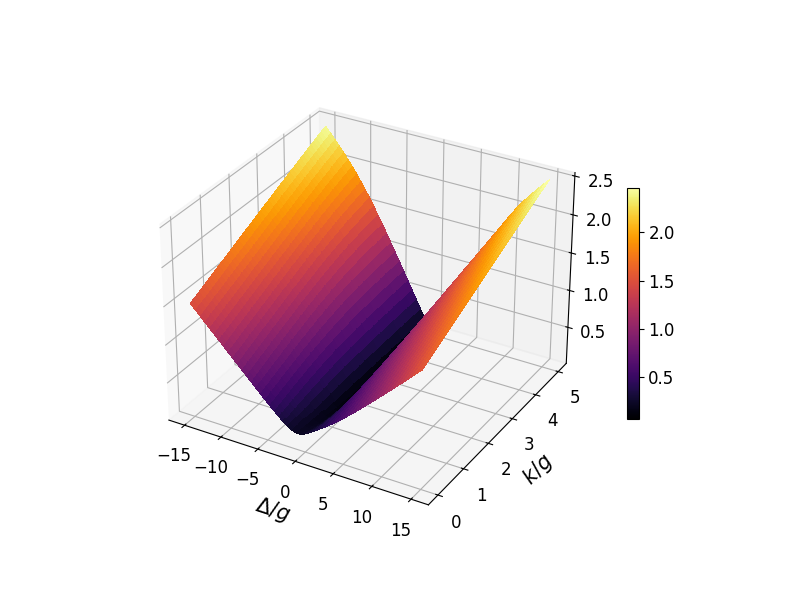
\includegraphics[width=\textwidth]{figuras/ch4/omega23 x=0.png}
%         \caption{}
%         \label{fig4:rabi chi}
%     \end{subfigure}
%     \hfill
%     \begin{subfigure}{0.3\textwidth}
%         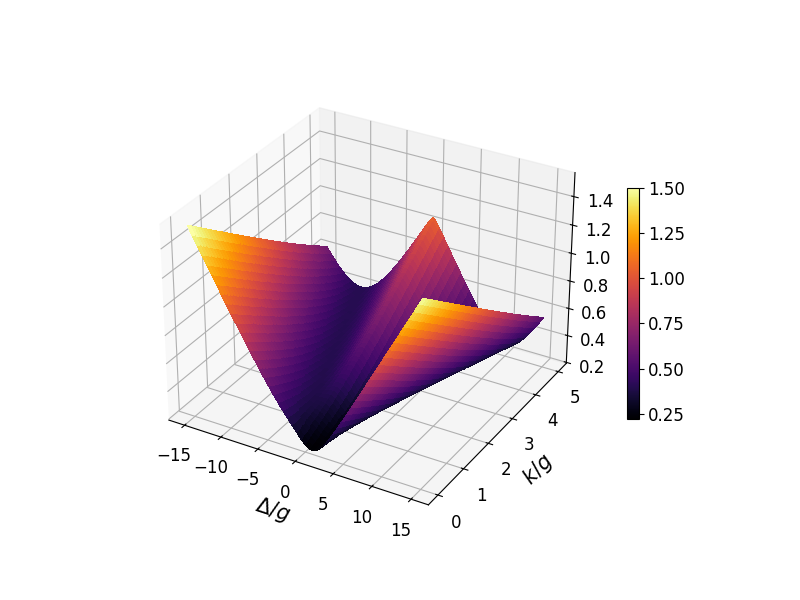
\includegraphics[width=\textwidth]{figuras/ch4/omega31 x=0.png}
%         \caption{}
%         \label{fig4:rabi chi}
%     \end{subfigure}
%     \caption{Frecuencias de Rabi en función del detunning, para diferentes valores de $\chi/g\in[0,5]$ y $k-J=0.5g$. A la izquierda $\Omega_{12}$ y a la derecha $\Omega_{23}$ y $\Omega_{13}$}
%     \label{}
% \end{figure}

Al cambiar las no linealidades del medio $\chi$ (figura \ref{fig4:rabi 1 chi} y \ref{sub@fig4:rabi 2 chi}), la frecuencia $\Omega^{(2)}_{12}$ se comporta de manera similar a la frecuencia de Rabi del JC de 1 átomo, que es también igual a la $\Omega^{(1)}$. En ambos casos la diferencia de energía tiene un máximo que se desplaza lateralmente al aumentar el parámetro $\chi\in[0,5g]$, pero presenta una sutil diferencia, ya que también el máximo aumenta en valor absoluto. En la figura \ref{fig4:rabi 1 k} y \ref{sub@fig4:rabi 2 k} se explora el efecto de modificar $k-J\in [0,5g]$, donde el máximo ya no se desplaza lateralmente, sino que aumenta en valor absoluto. Por otro lado, en los paneles derechos, se puede analizar qué sucede con las frecuencias $\Omega^{(2)}_{23}$ y $\Omega^{(2)}_{31}$ al aumentar $\chi$ (Fig. \ref{fig4:rabi 2 chi}) y $k-J$ (Fig. \ref{fig4:rabi 2 k}). Es interesante notar como al aumentar $\chi$, se comienza a observar un máximo y mínimo local para la frecuencia $\Omega^{(2)}_{23}$ (rama superior). Similarmente, pero en la rama inferior, se observa este mismo comportamiento al aumentar $k-J$.


La dinámica para el caso de $N\geq2$ es compleja, ya que ahora se tienen 3 frecuencias diferentes, y predecir que sucede para cada combinación de parámetros y para cada condición inicial se hace muy complicado, por lo tanto, el análisis para estos casos no es profundo, sino cualitativo. Lo que se puede distinguir es que cuando $\chi$, $k-J>g$, se comienzan a observar estos mínimos y máximos locales en las frecuencias, y se puede estudiar cuál es el efecto que tiene esto en el entrelazamiento de los átomos, y también si hay alguna relación entre los parámetros, por ejemplo como se encontró para el caso de 1 átomo (y para el subespacio de N=1) que hay una clara relación entre el detunning $\Delta$ y el medio $\chi$. En particular, es de interés encontrar una condición de robustez, similar a la Ec. (\ref{ec3:condicion robuestez 1 atomo}).

\section{Dinámica de entrelazamiento}

De manera general, se puede estudiar el entrelazamiento del sistema total. La dificultad que se encuentra es que, la entropía de von Neumann para sistemas mixtos, ya no es una buena medida para estudiar el entrelazamiento. Como mencionamos antes, una medida que sirve es la \textit{Entanglement of Formation} dada por la Ec. (\ref{ec4:entanglement}). Esta definición formal es complicada de aplicar para sistemas tripartitos (en general para sistemas de más de dos partes). Por lo tanto, en este capítulo, se estudia el entrelazamiento entre los dos átomos dentro de la cavidad. De esta forma, el sistema de estudio es bipartito, ya que la cavidad pasa a tomar el rol de entorno. Para sistemas bipartitos, la medida de entrelazamiento utilizada es la concurrencia. Si bien se traza sobre la cavidad y pasa a formar parte del entorno, su dinámica sigue siendo relevante, ya que la solución la tiene en cuenta, y al final se toma traza parcial para obtener esta cantidad. Por lo tanto hay efectos no-markovianos en la concurrencia, ya que las excitaciones y la información que se transmiten de los átomos a la cavidad, no se pierde como si fuera un entorno con infinitos grados de libertad. Por lo tanto, para estudiar la dinámica de entrelazamiento entre los dos átomos $\rho_{AB}=\tr_C\{\rho\}$, se utiliza la concurrencia como medida de entrelazamiento definida por la Ec. (\ref{ec4:concurrencia}) ($0\leq C_{AB} \leq 1$).

Lo primero que se analiza son los efectos de las interacciones entre los átomos. Se diferencian dos regímenes, el de Strong Interacting (SI) y Weak Interacting (WI), refiriéndose a la interacción entre los átomos con respecto a la cavidad. El SI será cuando la interacción entre los átomos es fuerte en comparación con la cavidad, es decir $k-J>g$, y WI con $k,J<g$. Ya que no se encontró un límite muy claro, se utilizará un valor representativo de cada régimen, $k-J=0.5g$ y $k-J=2.5g$ respectivamente, además de utilizar un parámetro del entorno $\gamma=0.25g$. Para ilustrar las diferencias entre condiciones iniciales, y para seguir con el paralelismo con el caso de 1 átomo, se considerarán únicamente las siguientes condiciones iniciales:
\begin{itemize}
    \item $\frac{1}{\sqrt{2}}(\ket{eg0}+\ket{ge0})$ para seguir el paralelismo con el JCM de 1 átomo 
    \item $\frac{1}{\sqrt{2}}(\ket{eg1}+\ket{ge1})$ para comparar con el anterior y explorar el subespacio $N=2$.
    %\item $\ket{ee0+gg2}$ para ver otra condición inicial con $N=2$ en donde los átomos \textbf{no} están entrelazados
\end{itemize}

Para comparar el efecto de los parámetros entre sí, todos los gráficos que se muestran en el resto del capítulo estarán caracterizados por un acoplamiento con el entorno de $\gamma=0.25g$, y todos los tiempos estarán normalizados según un periodo $T_0=2\pi/\Omega_0$ con $\Omega_0=\Omega^{(1)}(\Delta=0,\chi=0,k-J=0)$.
\subsection{Condición inicial $\frac{1}{\sqrt{2}}(\ket{eg0}+\ket{ge0})$}
Primero se analiza la dinámica para el estado inicial $\ket{\phi_2^{(1)}}$ de la base $\mathcal{B}_1$.
\subsubsection{\underline{Dependencia con el detunning}}
\begin{figure}[h!]
    \centering
    \begin{subfigure}{0.49\textwidth}
        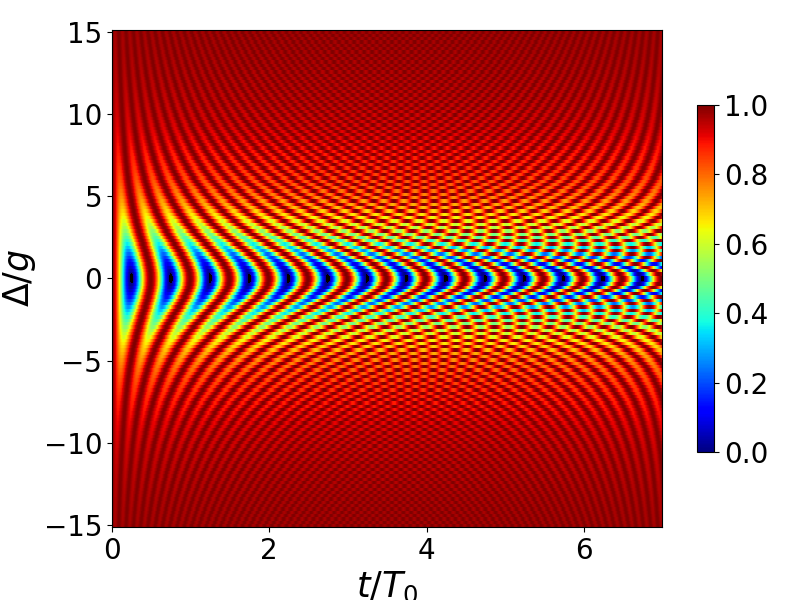
\includegraphics[width=\textwidth]{figuras/ch4/concu/delta/eg0+ge0 k=0.0g x=0.0g J=0.0g gamma=0.25g concu delta uni.png}
        \caption{}
        \label{fig4:concu detunning 0 uni}
    \end{subfigure}
    \hfill
    \begin{subfigure}{0.49\textwidth}
        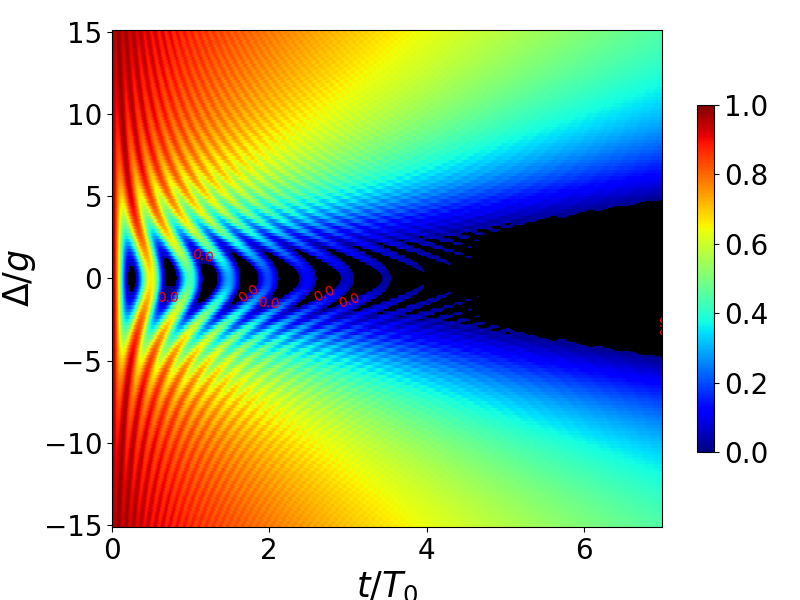
\includegraphics[width=\textwidth]{figuras/ch4/concu/delta/eg0+ge0 k=0.0g x=0.0g J=0.0g gamma=0.25g concu delta dis.png}
        \caption{}
        \label{fig4:concu detunning 0 dis}
    \end{subfigure}
    \vfill
        \begin{subfigure}{0.49\textwidth}
        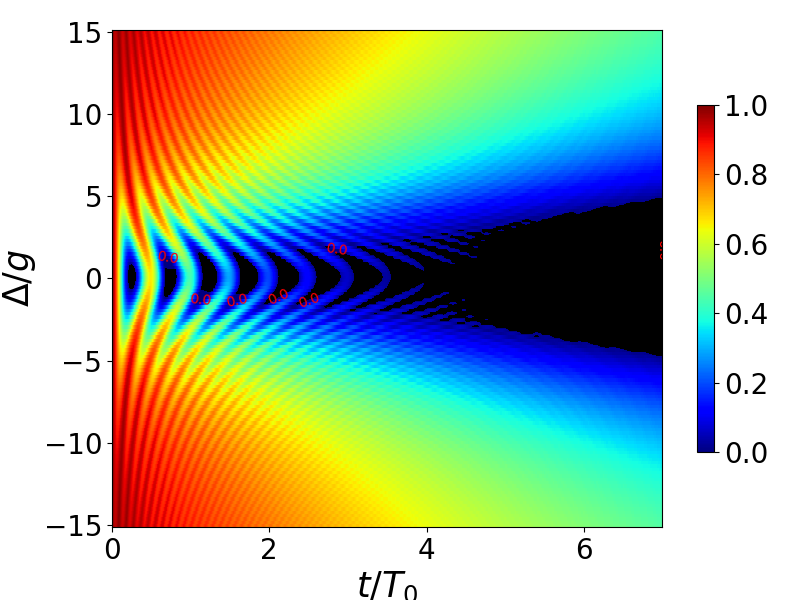
\includegraphics[width=\textwidth]{figuras/ch4/concu/delta/eg0+ge0 k=0.0g x=0.1g J=0.0g gamma=0.25g concu delta dis.png}
        \caption{$\chi=0.1g$}
        \label{fig4:concu detunning x1}
    \end{subfigure}
    \hfill
    \begin{subfigure}{0.49\textwidth}
        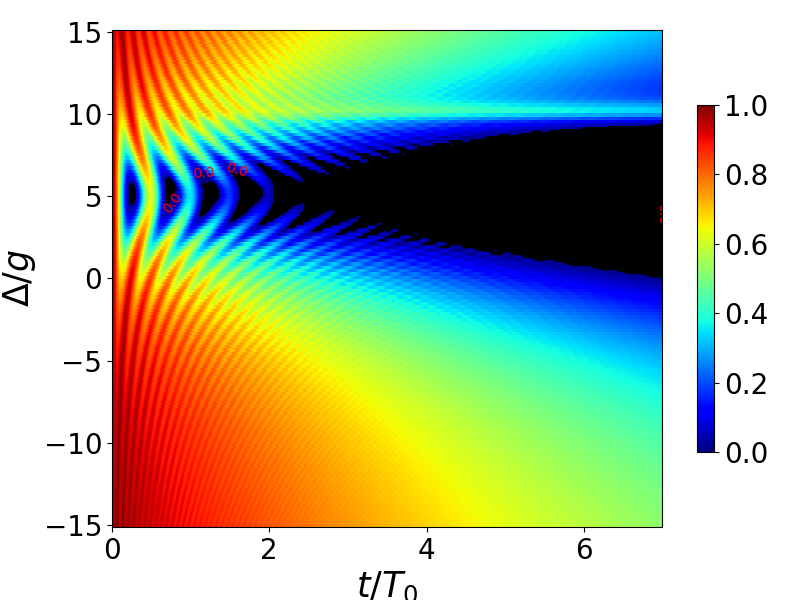
\includegraphics[width=\textwidth]{figuras/ch4/concu/delta/eg0+ge0 k=0.0g x=5.0g J=0.0g gamma=0.25g concu delta dis.png}
        \caption{$\chi=5g$}
        \label{fig4:concu detunning x2}
    \end{subfigure}
    \vfill
    \begin{subfigure}{0.49\textwidth}
        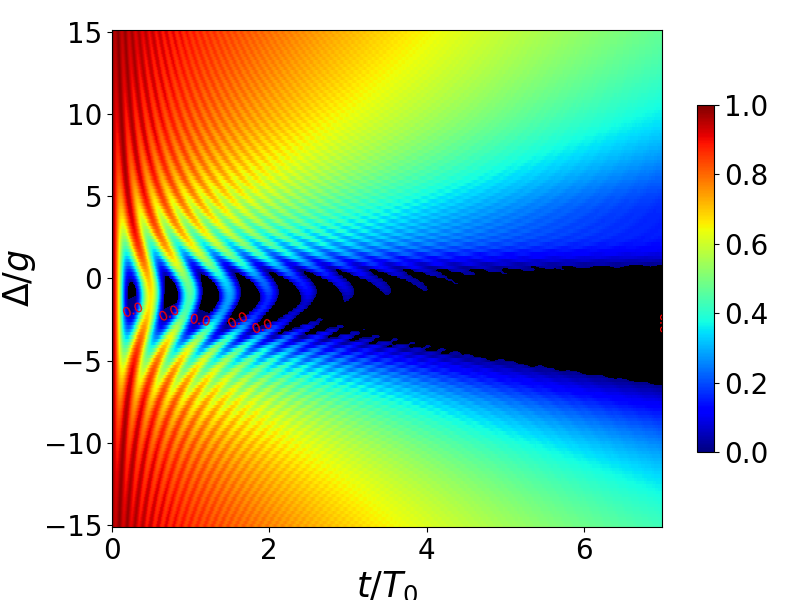
\includegraphics[width=\textwidth]{figuras/ch4/concu/delta/eg0+ge0 k=0.5g x=0.0g J=0.0g gamma=0.25g concu delta dis.png}
        \caption{$k-J=0.5g$}
        \label{fig4:concu detunning k1}
    \end{subfigure}
    \hfill
    \begin{subfigure}{0.49\textwidth}
        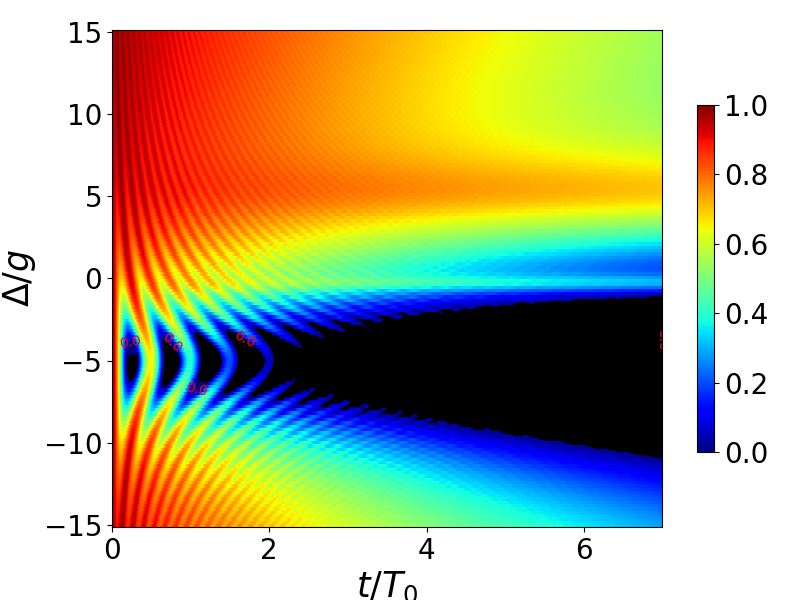
\includegraphics[width=\textwidth]{figuras/ch4/concu/delta/eg0+ge0 k=2.5g x=0.0g J=0.0g gamma=0.25g concu delta dis.png}
        \caption{$k-J=2.5g$}
        \label{fig4:concu detunning k2}
    \end{subfigure}
    \caption{Dinámica de entrelazamiento para el estado inicial $\frac{1}{\sqrt{2}}(\ket{eg0}+\ket{ge0})$, en función del detunning, para diferentes parámetros. Dinámica sin pérdidas: (a) $\chi=k-J=0$. Dinámica con pérdidas: (b) $\chi=k-J=0$; (c) $\chi=0.1g$, $k-J=0$; (d) $\chi=5g$, $k-J=0$; (e) $\chi=0$, $k-J=0.5g$; (f) $\chi=0$, $k-J=2.5g$.}
    \label{fig4:concu detunning 0}
\end{figure}
En la figura \ref{fig4:concu detunning 0} se observa la evolución de la concurrencia para la condición inicial $\frac{1}{\sqrt{2}}(\ket{eg0}+\ket{ge0})$, cuyo entrelazamiento entre los átomos es máximo. El eje x es el tiempo, y el eje y es el detunning $\Delta/g$. En el panel \ref{fig4:concu detunning 0 uni} se muestra el caso sin pérdidas. Lo primero que se aprecia es que la figura es simétrica sobre $\Delta=0$ (caso resonante), y las oscilaciones son de menor frecuencia pero de mayor amplitud. A medida que se aumenta el valor absoluto del detunning, las oscilaciones son de mayor frecuencia y menor amplitud. Consecuentemente, al tomar la dinámica disipativa, en el panel (\ref{sub@fig4:concu detunning 0 dis}), las oscilaciones siguen estando, pero ahora su máximo disminuye con el tiempo. Esto es de esperar, ya que la cavidad deja escapar fotones y el estado del sistema se hace mixto. Un estado mixto ya no es entrelazado, porque no hay coherencias, entonces se observa el deterioro del entrelazamiento a medida que el tiempo avanza. Hay otros dos comportamientos notables. 
Por un lado, se observa como el máximo del entrelazamiento decae más lentamente para valores más altos del detunning, esto se debe a la naturaleza de la dinámica poblacional. Al aumentar el detunning, como se vio anteriormente, uno de los efectos principales es que las oscilaciones entre los estados tienen poca amplitud, y en este caso, esto implica que si bien el estado $\ket{gg1}$ tiene amplitud no nula, principalmente la probabilidad está concentrada en el estado inicial, que no sufre decoherencia por pérdida de fotones, ya que no tiene fotones en la cavidad. Entonces, mientras mayor el detunning, menor la probabilidad de encontrar al sistema en el estado $\ket{gg1}$, y por lo tanto tiene pocas probabilidades de perder fotones. Por otro lado, un efecto frecuente en este tipo de sistemas, es la muerte y reanimación súbita del entrelazamiento, que se nombran SDE (Sudden Death Effect) y SBE (Sudden Birth Effect) por sus siglas en inglés. En el caso disipativo, se marcaron zonas en negro. Estas zonas o regiones muestran cómo el entrelazamiento \textit{muere} durante un tiempo finito y revive luego. Este efecto es sorprendente, ya que se espera que las coherencias, responsables en gran medida del entrelazamiento entre átomos, decaigan asintóticamente. Este efecto muestra que esto no es así para algunos sistemas, y aún cuando las coherencias son distintas de cero, el entrelazamiento puede ser nulo durante un tiempo, y luego reaparecer súbitamente. La razón por la que aparece este fenómeno es que se está tomando traza parcial sobre la cavidad, lo que hace que algunas coherencias desaparezcan. Aún así, no se entiende bien el por qué de este efecto \cite{Roncaglia2008}.

La pregunta natural que sigue es si cambiar los parámetros $\chi$ y $k-J$, cambian la forma de la figura \ref{fig4:concu detunning 0}. En las figuras \ref{fig4:concu detunning x1}-\ref{sub@fig4:concu detunning k2} se muestra nuevamente la dinámica de entrelazamiento en función del detunning, donde se modificó alguno de los parámetros.

En el las figuras \ref{fig4:concu detunning x1} y \ref{fig4:concu detunning x2} se muestran dos casos en donde se puso de manifiesto la no linealidad del medio, cuyos parámetros son $\chi=0.1g$ y $\chi=5g$ respectivamente, ambos casos en presencia del entorno. Al comparar con la figura \ref{fig4:concu detunning 0 dis}, la forma cambia al aumentar las no linealidades, y la figura ya no es simétrica. De todas formas, cerca del centro ($\Delta/g=5$) el comportamiento es similar, y por lo tanto podría esperarse que este eje será el caso coherente, que en analogía con la sección \ref{sec3:fg disipacion}, puede ser una posible condición de robustez para la fase geométrica. Esto se analizará más adelante. En los paneles \ref{fig4:concu detunning k1} y \ref{fig4:concu detunning k2} se muestra el cambio al considerar acoplamiento entre los átomos, dados por una intensidad de $k-J=0.5g$ y $k-J=2.5g$ respectivamente. Nuevamente hay un desplazamiento, que se comporta igual que en el caso anterior, pero ahora el desplazamiento del eje es el doble que el aumento del parámetro de estudio, por ejemplo, si $k-J=2.5g$, entonces la figura se desplaza y su \textit{centro} está en $\Delta_0=-2(k-J)=-5g$. Esto no es tan sorprendente si se observa la expresión de la energía Ec. (\ref{ec4:energias n1}), donde los parámetros $\chi$ y $\Delta$ aparecen con un factor $1/2$, mientras que $k-J$ no. 

La simetría de la figura se rompe en una dirección, y se ve como hay, en ambos casos, una franja donde el entrelazamiento parece mantenerse durante un periodo más largo de tiempo. Además, se observa cómo en el panel \ref{fig4:concu detunning k2} (que se corresponde con el caso $k-J=2.5g$), en la parte superior de la imagen, el entrelazamiento persiste mayor tiempo que su contraparte de menor interacción (panel \ref{fig4:concu detunning k1}) con $k-J=0.5g$.

Básicamente, el subespacio de $N=1$ se comporta igual que el Jaynes-Cummings de 1 átomo, pero donde se tiene un estado \textit{inerte}, el estado $\frac{1}{\sqrt{2}}(\ket{eg0}-\ket{ge0})$ que no interactúa con los otros dos. Esto puede ser de interés, porque usando como condición inicial el estado $\ket{\psi_0}=\cos\theta\ket{eg0}+\sin\theta\ket{ge0}$ que es combinación lineal de los estados $\frac{1}{\sqrt{2}}(\ket{eg0}\pm\ket{ge0})$, donde el estado simétrico evoluciona como siempre, y el antisimétrico no evoluciona, se encuentra una manera de mantener el entrelazamiento siempre por arriba de un cierto valor, que depende del valor de $\theta$, aún en presencia de decoherencia- Esto es porque el estado $\frac{1}{\sqrt{2}}(\ket{eg0}-\ket{ge0})$ es un estado que no sufre pérdidas.

\subsubsection{\underline{Dependencia con el Kerr}}
En la figura \ref{fig4:concu x 0} se muestra la dinámica de entrelazamiento en función de la no linealidad del medio. No hay diferencias mayores con la dependencia en $\Delta$ (figura \ref{fig4:concu detunning 0}). Nuevamente se observa que el efecto principal de modificar los parámetros es desplazar el centro donde se observan oscilaciones de mayor amplitud y SDE. Es interesante que también emergen asimetrías, y en particular, en las figuras \ref{fig4:concu x d2} y \ref{sub@fig4:concu x k2} se observan franjas de entrelazamiento robustas para $\chi=\Delta/2=2.5g$ en la primera, y para $\chi=\Delta=0$ en la segunda.

\begin{figure}[h!]
    \centering
    \begin{subfigure}{0.49\textwidth}
        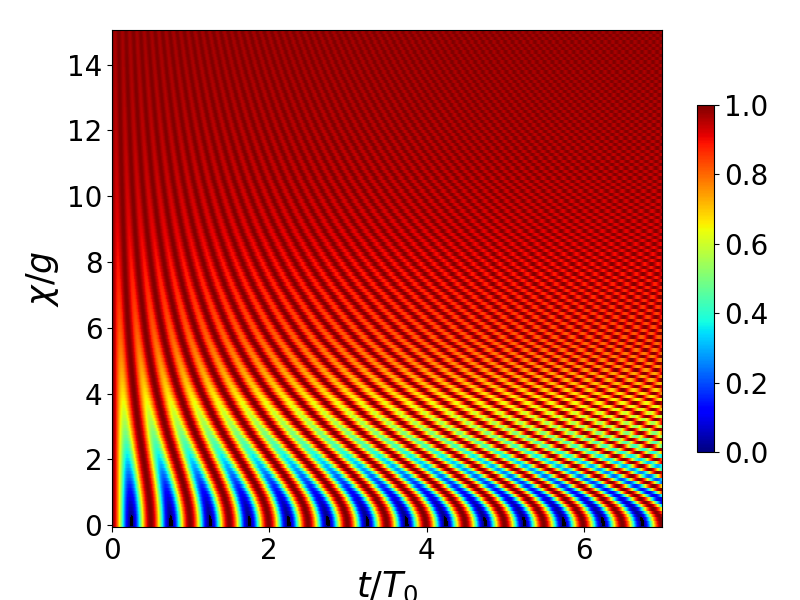
\includegraphics[width=\textwidth]{figuras/ch4/concu/chi/eg0+ge0 d=0.0g k=0.0g J=0.0g gamma=0.25g concu chi uni.png}
        \caption{}
        \label{fig4:concu x 0 uni}
    \end{subfigure}
    \hfill
    \begin{subfigure}{0.49\textwidth}
        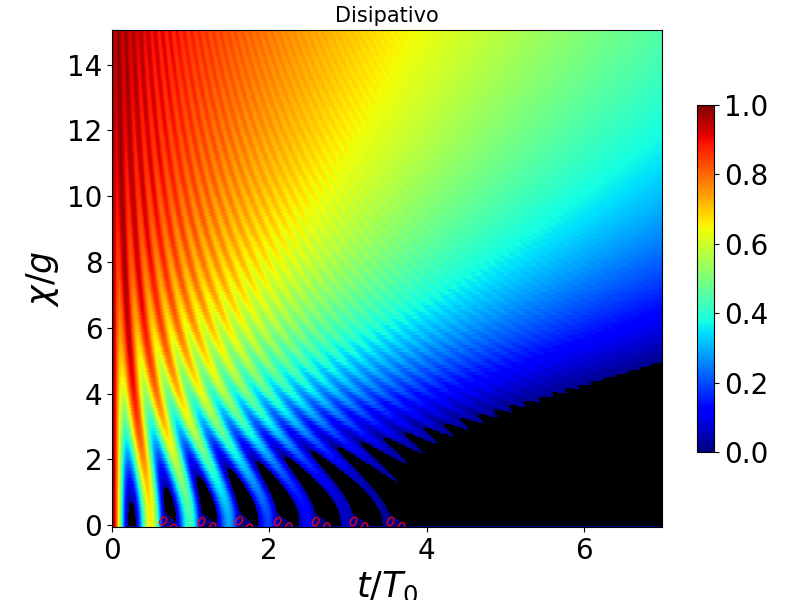
\includegraphics[width=\textwidth]{figuras/ch4/concu/chi/eg0+ge0 d=0.0g k=0.0g J=0.0g gamma=0.25g concu chi dis.png}
        \caption{}
        \label{fig4:concu x 0 dis}
    \end{subfigure}
    \vfill
    \begin{subfigure}{0.49\textwidth}
        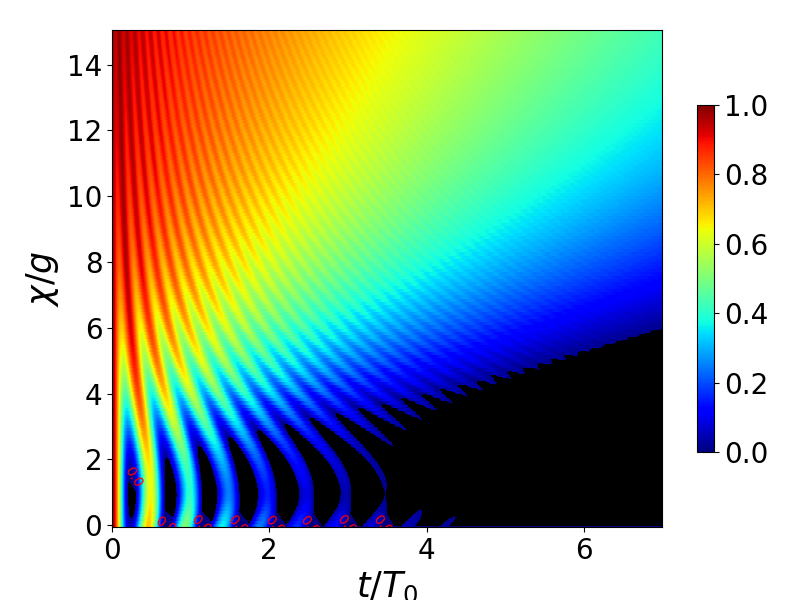
\includegraphics[width=\textwidth]{figuras/ch4/concu/chi/eg0+ge0 d=1.0g k=0.0g J=0.0g gamma=0.25g concu chi dis.png}
        \caption{$\Delta=1g$}
        \label{fig4:concu x d1}
    \end{subfigure}
    \hfill
    \begin{subfigure}{0.49\textwidth}
        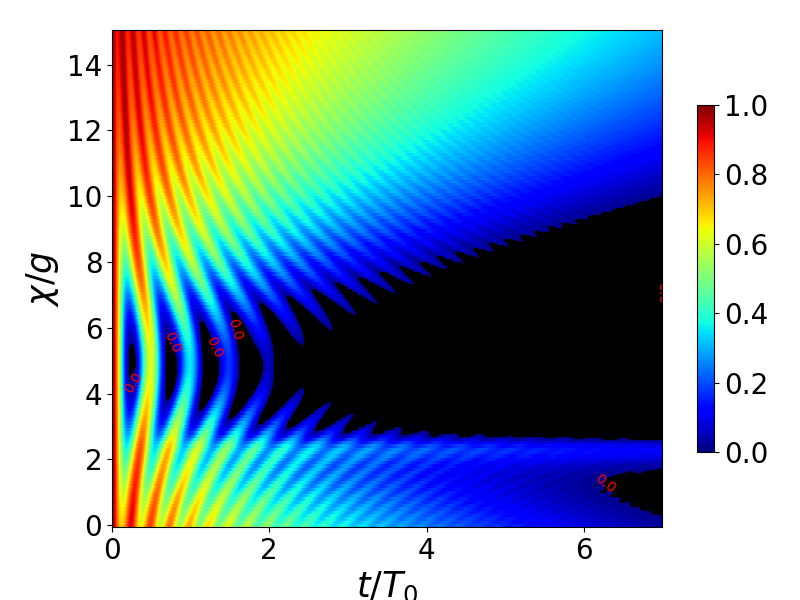
\includegraphics[width=\textwidth]{figuras/ch4/concu/chi/eg0+ge0 d=5.0g k=0.0g J=0.0g gamma=0.25g concu chi dis.png}
        \caption{$\Delta=5g$}
        \label{fig4:concu x d2}
    \end{subfigure}
    \vfill
    \begin{subfigure}{0.49\textwidth}
        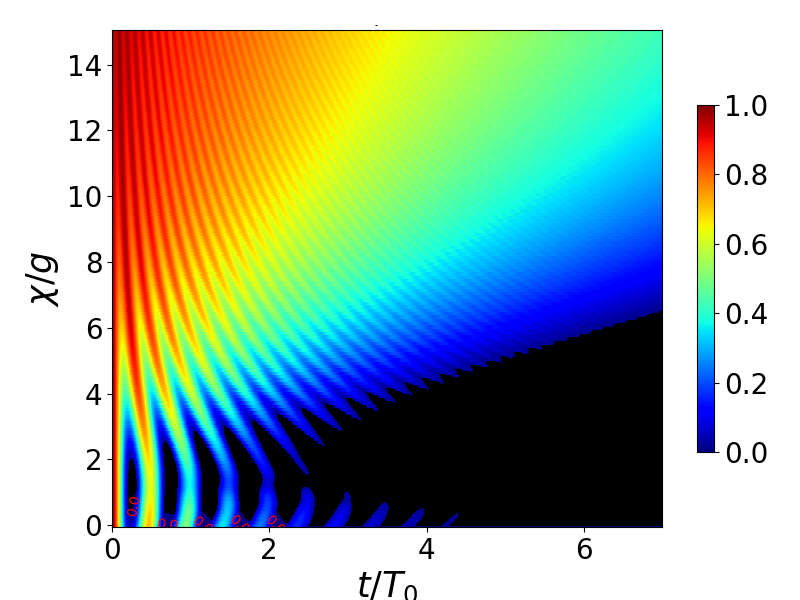
\includegraphics[width=\textwidth]{figuras/ch4/concu/chi/eg0+ge0 d=0.0g k=0.5g J=0.0g gamma=0.25g concu chi dis.png}
        \caption{$k-J=0.5g$}
        \label{fig4:concu x k1}
    \end{subfigure}
    \hfill
    \begin{subfigure}{0.49\textwidth}
        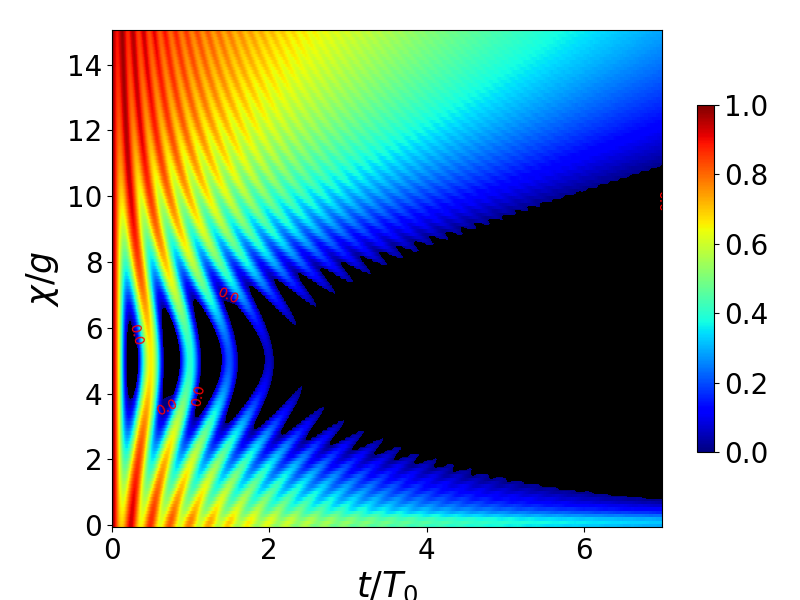
\includegraphics[width=\textwidth]{figuras/ch4/concu/chi/eg0+ge0 d=0.0g k=2.5g J=0.0g gamma=0.25g concu chi dis.png}
        \caption{$k-J=2.5g$}
        \label{fig4:concu x k2}
    \end{subfigure}
    \caption{Dinámica de entrelazamiento para el estado inicial $\frac{1}{\sqrt{2}}(\ket{eg0}+\ket{ge0})$, en función del detunning, y para $\chi=k-J=0$.(a) Dinámica sin pérdidas,(b) Dinámica con pérdidas. Luego, con pérdidas, (c)$\Delta=g$, $k-J=0$; (d) $\Delta=5g$, $k-J=0$; (e) $\Delta=0$, $k-J=0.5g$; (f) $\Delta=0$, $k-J=2.5g$.}
    \label{fig4:concu x 0}
\end{figure}

Esto reafirma que en el espacio de $N=1$, el medio Kerr es muy similar al detunning. 
\newpage
\subsubsection{\underline{Dependencia con la interacción entre átomos}}
\begin{figure}[h!]
    \centering
    \begin{subfigure}{0.49\textwidth}
        \includegraphics[width=\textwidth]{figuras/ch4/concu/k/eg0+ge0 d=0.0g x=0.0g J=15.0g gamma=0.25g concu k uni.png}
        \caption{$\Delta=\chi=0$}
        \label{fig4:concu k 0 uni}
    \end{subfigure}
    \hfill
    \begin{subfigure}{0.49\textwidth}
        \includegraphics[width=\textwidth]{figuras/ch4/concu/k/eg0+ge0 d=0.0g x=0.0g J=15.0g gamma=0.25g concu k dis.png}
        \caption{$\Delta=\chi=0$}
        \label{fig4:concu k 0 dis}
    \end{subfigure}
    \vfill
    \begin{subfigure}{0.49\textwidth}
        \includegraphics[width=\textwidth]{figuras/ch4/concu/k/eg0+ge0 d=1.0g x=0.0g J=15.0g gamma=0.25g concu k dis.png}
        \caption{$\Delta=1g$}
        \label{fig4:concu k d1}
    \end{subfigure}
    \hfill
    \begin{subfigure}{0.49\textwidth}
        \includegraphics[width=\textwidth]{figuras/ch4/concu/k/eg0+ge0 d=5.0g x=0.0g J=15.0g gamma=0.25g concu k dis.png}
        \caption{$\Delta=5g$}
        \label{fig4:concu k d2}
    \end{subfigure}
    \vfill
    \begin{subfigure}{0.49\textwidth}
        \includegraphics[width=\textwidth]{figuras/ch4/concu/k/eg0+ge0 d=0.0g x=0.5g J=15.0g gamma=0.25g concu k dis.png}
        \caption{$\chi=0.5g$}
        \label{fig4:concu k x1}
    \end{subfigure}
    \hfill
    \begin{subfigure}{0.49\textwidth}
        \includegraphics[width=\textwidth]{figuras/ch4/concu/k/eg0+ge0 d=0.0g x=5.0g J=15.0g gamma=0.25g concu k dis.png}
        \caption{$\chi=5g$}
        \label{fig4:concu k x2}
    \end{subfigure}
    \caption{Dinámica de entrelazamiento para el estado inicial $\frac{1}{\sqrt{2}}(\ket{eg0}+\ket{ge0})$, en función de la interacción entre los átomos (a) Dinámica sin pérdidas con $\Delta=\chi=0$.  Dinámica con pérdidas (b) $\Delta=\chi=0$; (c) $\Delta=g$, $\chi=0$; (d) $\Delta=5g$, $\chi=0$; (e) $\Delta=0$, $\chi=0.5g$; (f) $\Delta=0$, $\chi=5g$.}
    \label{fig4:concu k 0}
\end{figure}
Desde el comienzo ya se puede ver como al aumentar el valor absoluto de la interacción el comportamiento es el mismo que en los otros dos casos, donde aumenta la frecuencia y disminuye la amplitud conservando el entrelazamiento inicial, pero en este caso el  comportamiento se ve acentuado. 


La interacción entre los átomos conserva mejor el entrelazamiento. Esto también se observa cuando se agrega la disipación, en comparación con las otras interacciones. En la figura \ref{fig4:concu k 0 uni} se ve como se conserva mejor el entrelazamiento.

En las figuras \ref{fig4:concu k d1}-\ref{sub@fig4:concu k x2} se observan los efectos que tienen los otros dos parámetros en la dinámica. Por un lado, vemos que aumentar el detunning \ref{fig4:concu k d1} desplaza el centro hacia abajo pero no parece haber mucha diferencia. Al seguir aumentando la desintonía \ref{fig4:concu k d2}, el centro se sigue desplazando y podemos ver que éste se desplaza la mitad que lo que aumenta $\Delta$. Además, la estructura pierde la simetría y se observa una franja en la parte superior donde el entrelazamiento se conserva mejor. Este valor parece corresponderse con $+\Delta/2$. 

Juntando estos análisis, y mirando las expresiones de las energías Ec. (\ref{ec4:autoenergias}), es evidente que la condición de robustez para los estados de una excitación $N=1$ se da cuando
\begin{equation}
    \label{ec4:condicion0}
    \Delta-\chi+2(k-J)=0.
\end{equation}

En particular, cuando se cumple esta condición, los autovectores del Hamitloniano son
\begin{equation}
    \ket{u_{1,2}^{(1)}}=\frac{1}{\sqrt{2}}(\ket{gg1}\mp \frac{\ket{eg0}+\ket{ge0}}{\sqrt{2}})=\frac{\ket{\phi_1^{(1)}}\mp\ket{\phi_2^{(1)}}}{\sqrt{2}},
\end{equation}
que son estados entrelazados en la base utilizada. Si solo consideramos que hay dos estados relevantes, entonces estos autovectores son MES.

Es interesante que al cambiar las no linealidades, en las figuras \ref{fig4:concu k d2} y \ref{sub@fig4:concu k x2}, vemos que el efecto es exactamente el mismo, pero el desplazamiento es ahora en el otro sentido, y las condiciones de degeneración siguen siendo las mismas, a menos de un signo.
\subsection{Condición inicial $\frac{1}{\sqrt{2}}(\ket{eg1}+\ket{ge1})$}

\subsubsection{\underline{Dependencia con el detunning}}

Ahora se estudia la dinámica para el estado simétrico en el subespacio de $N=2$. Igual que en el caso anterior, la figura \ref{fig4:concu detunning 1} muestra la evolución unitaria a la izquierda, y la disipativa a la derecha. En este subespacio hay más estructura, y si bien sigue siendo simétrico con respecto al eje $\Delta=0$, la forma es más complicada, y en el caso unitario también se observan regiones que presentan SDE, cosa que para $N=1$ no aparecen. Al igual que antes, al aumentar el detunning las oscilaciones son de mayor frecuencia y menor amplitud, conservando mejor el entrelazamiento. La razón es la misma: si bien ahora el estado $\frac{1}{\sqrt{2}}(\ket{eg1}+\ket{ge1})$ si puede perder fotones, al hacerlo cae al estado $\frac{1}{\sqrt{2}}(\ket{eg0}+\ket{ge0})$, que tiene el mismo entrelazamiento, y los otros dos estados del subespacio $\ket{gg2}$ decaen al $\ket{gg1}$, y $\ket{ee0}$ no tiene fotones así que no pierde excitaciones. Por lo tanto, en el caso de alta desintonía, el comportamiento es similar al de anterior: las oscilaciones no tienen mucha amplitud y por lo tanto la probabilidad está concentrada casi toda en el estado $\frac{1}{\sqrt{2}}(\ket{eg1}+\ket{ge1})$, que al perder un fotón decae al estado $\frac{1}{\sqrt{2}}(\ket{eg0}+\ket{ge0})$ (junto con sus coherencias), entonces el entrelazamiento es el mismo.
\begin{figure}[H]
    \centering
    \begin{subfigure}{0.49\textwidth}
        \includegraphics[width=\textwidth]{figuras/ch4/concu/delta/eg1+ge1 k=0.0g x=0.0g J=0.0g gamma=0.25g concu delta uni.png}
        \caption{}
        \label{fig4:concu detunning 1 uni}
    \end{subfigure}
    \hfill
    \begin{subfigure}{0.49\textwidth}
        \includegraphics[width=\textwidth]{figuras/ch4/concu/delta/eg1+ge1 k=0.0g x=0.0g J=0.0g gamma=0.25g concu delta dis.png}
        \caption{}
        \label{fig4:concu detunning 1 dis}
    \end{subfigure}
    \vfill
    \begin{subfigure}{0.49\textwidth}
        \includegraphics[width=\textwidth]{figuras/ch4/concu/delta/eg1+ge1 k=0.0g x=0.1g J=0.0g gamma=0.25g concu delta dis.png}
        \caption{$\chi=0.1g$}
        \label{fig4:concu detunning 1 x1}
    \end{subfigure}
    \hfill
    \begin{subfigure}{0.49\textwidth}
        \includegraphics[width=\textwidth]{figuras/ch4/concu/delta/eg1+ge1 k=0.0g x=5.0g J=0.0g gamma=0.25g concu delta dis.png}
        \caption{$\chi=5g$}
        \label{fig4:concu detunning 1 x2}
    \end{subfigure}
    \vfill
    \begin{subfigure}{0.49\textwidth}
        \includegraphics[width=\textwidth]{figuras/ch4/concu/delta/eg1+ge1 k=0.5g x=0.0g J=0.0g gamma=0.25g concu delta dis.png}
        \caption{$k-J=0.5g$}
        \label{fig4:concu detunning 1 k1}
    \end{subfigure}
    \hfill
    \begin{subfigure}{0.49\textwidth}
        \includegraphics[width=\textwidth]{figuras/ch4/concu/delta/eg1+ge1 k=2.5g x=0.0g J=0.0g gamma=0.25g concu delta dis.png}
        \caption{$k-J=2.5g$}
        \label{fig4:concu detunning 1 k2}
    \end{subfigure}
    \caption{Dinámica de entrelazamiento para el estado inicial $\frac{1}{\sqrt{2}}(\ket{eg0}+\ket{ge0})$, en función del detunning, y para $\chi=k-J=0$. (a) Dinámica sin pérdidas, (b) Dinámica con pérdidas. (\ref{sub@fig4:concu detunning x1}) $\chi=0.1g$, $k-J=0$; (\ref{sub@fig4:concu detunning x2}) $\chi=5g$, $k-J=0$; (\ref{sub@fig4:concu detunning k1}) $\chi=0$, $k-J=0.5g$; (\ref{sub@fig4:concu detunning k2}) $\chi=0$, $k-J=2.5g$ }
    \label{fig4:concu detunning 1}
\end{figure}

Este subespacio de mayor excitación es relevante, ya que las energías de los estados presentan máximos y mínimos locales en función de los parámetros del problema (figuras \ref{fig4:frecuencias de rabi}), lo que cambia drásticamente el entrelazamiento al modificar los valores de los parámetros.

En las figuras \ref{fig4:concu detunning 1 x1}-\ref{sub@fig4:concu detunning 1 k2} se muestran diferentes casos. En la primera fila los casos con medio Kerr cuyos parámetros son $\chi=0.1g$ y $\chi=5g$ respectivamente. En la figura \ref{fig4:concu detunning x1} correspondiente a $\chi=0.1g$, no se observa ningún cambio significativo con respecto al caso $\chi=0$, es muy pequeño para ser notado y la estructura queda igual. Pero al aumentar mucho la no linealidad del medio, se comienza a observar el desdoblamiento en las energías, y los máximos y mínimos locales comienzan a tomar importancia. En la figura \ref{fig4:concu detunning 1 x2} se ve como hay dos zonas en donde las oscilaciones tienen gran amplitud y poca frecuencia, similar al caso \textit{resonante}. Esto se puede explicar con el desdoblamiento de energías. Hay dos mínimos en las frecuencias de Rabi que participan en este proceso, que están cerca de $\Delta_1=5g$ y $\Delta_2=15g$ aproximadamente. Haciendo una analogía con el caso de 1 átomo, donde vimos que la condición de robustez se daba para $\Delta=\chi(2n_c-1)$ (ver (\ref{sec3:medio kerr})) y recordando que esta condición se obtiene de la diferencia entre las contribuciones diagonales del Hamiltoniano, entonces en este caso, se puede hacer lo mismo y obtener dos condiciones. La primera con $\chi n_c^2-\chi(n_c-1)^2=\chi(2n_c-1)$ que es igual a la del caso de $N=1$, y la segunda con $\chi(n_c-1)^2-\chi(n_c-2)^2=\chi(2n_c-3)$. Sustituyendo $n=2$, la condición se da para $\Delta=\chi$ y $\Delta=3\chi$, que es justo donde se aprecian los mínimos. Si bien el segundo mínimo de $3\chi$ parece ser menos pronunciado, esta analogía funciona bien.

Si se hace esta resta pero ahora con $\chi=0$ y nos concentramos en $k-J$, la condición se da cuando $\Delta=\pm 2(k-J)$, que es donde se observan los mínimos del entrelazamiento en la figura \ref{fig4:concu detunning 1 k2}. En general entonces, se puede decir que esta condición de menor frecuencia y mayor amplitud de oscilación se da cuando las energías de los estados están cerca de la degeneración, y como hay 3 estados que interactúan siempre por medio del estado del medio (el $\frac{1}{\sqrt{2}}(\ket{egn}+\ket{gen})$), entonces se dan en el caso general cuando se satisface que:

\begin{equation}
    \Delta-\chi(2n-1)+2(k-J)=0,
    \label{ec4:condicion 1}
\end{equation}
que se corresponde con la degeneración entre las energías del estado $\ket{ggn}$ y $\frac{1}{\sqrt{2}}(\ket{eg,n-1}+\ket{ge,n-1})$, y en el otro caso:
\begin{equation}
    \Delta-\chi(2n-3)-2(k-J)=0,
    \label{ec4:condicion 2}
\end{equation}
que se corresponde con los estados $\frac{1}{\sqrt{2}}(\ket{eg,n-1}+\ket{ge,n-1})$ y $\ket{ee,n-2}$. También, se puede dar que los tres estados están degenerados si se cumplen las dos condiciones simultáneamente.

La tercera condición que se puede dar es cuando los estados $\ket{ggn}$ y $\ket{ee,n-2}$ son degenerados. Si bien estos no interactúan directamente entre sí, el estado $\frac{1}{\sqrt{2}}(\ket{eg1}+\ket{ge1})$ interactúa con ambos, y si estos son degenerados, entonces están en igualdad de condiciones ante el estado inicial. Por lo tanto, la ultima condición se da cuando: 
\begin{equation}
    \Delta-2\chi(n-1)=0.
    \label{ec4:condicion 3}
\end{equation}
En particular para $n=2$ se tiene que $\Delta=2\chi$. En las figuras \ref{fig4:concu detunning 1 x2} y \ref{sub@fig4:concu detunning 1 k2}, se observa que cuando se cumple esta condición, el entrelazamiento es más fuerte ante el efecto del entorno.  

%\subsubsection{\underline{Condición inicial $\ket{ee0+gg2}$}}
%Esta condición inicial no tiene entrelazamiento inicial, ya que al tomar traza parcial sobre la cavidad, uno de los estados de la superposición tiene 0 fotones, y el otro 2, entonces el resultado de trazar sobre la cavidad en el instante inicial es que los átomos se encuentren en el estado máximamente mixto $\frac{1}{2}(\ketbra{ee}{ee}+\ketbra{gg}{gg})$, que no es entrelazado.

\subsubsection{\underline{Dependencia con el Kerr}}
Para la condición inicial $\frac{1}{\sqrt{2}}(\ket{eg1}+\ket{ge1})$ en función de $\chi$ se observan diferencias con el caso del detunning: las imágenes \ref{fig4:concu x 1} y \ref{fig4:concu detunning 1} tienen diferentes estructuras. Esto significa que ya no están en igualdad de condiciones el detunning y el medio, como era el caso de el subespacio de $N=1$.
\begin{figure}[h!]
    \centering
    \begin{subfigure}{0.49\textwidth}
        \includegraphics[width=\textwidth]{figuras/ch4/concu/chi/eg1+ge1 d=0.0g k=0.0g J=0.0g gamma=0.25g concu chi uni.png}
        \caption{}
        \label{fig4:concu x 1 uni}
    \end{subfigure}
    \hfill
    \begin{subfigure}{0.49\textwidth}
        \includegraphics[width=\textwidth]{figuras/ch4/concu/chi/eg1+ge1 d=0.0g k=0.0g J=0.0g gamma=0.25g concu chi dis.png}
        \caption{}
        \label{fig4:concu x 1 dis}
    \end{subfigure}
    \vfill
        \begin{subfigure}{0.49\textwidth}
        \includegraphics[width=\textwidth]{figuras/ch4/concu/chi/eg1+ge1 d=1.0g k=0.0g J=0.0g gamma=0.25g concu chi dis.png}
        \caption{$\Delta=1g$}
        \label{fig4:concu x 1 d1}
    \end{subfigure}
    \hfill
    \begin{subfigure}{0.49\textwidth}
        \includegraphics[width=\textwidth]{figuras/ch4/concu/chi/eg1+ge1 d=5.0g k=0.0g J=0.0g gamma=0.25g concu chi dis.png}
        \caption{$\Delta=5g$}
        \label{fig4:concu x 1 d2}
    \end{subfigure}
    \vfill
    \begin{subfigure}{0.49\textwidth}
        \includegraphics[width=\textwidth]{figuras/ch4/concu/chi/eg1+ge1 d=0.0g k=0.5g J=0.0g gamma=0.25g concu chi dis.png}
        \caption{$k-J=0.5g$}
        \label{fig4:concu x 1 k1}
    \end{subfigure}
    \hfill
    \begin{subfigure}{0.49\textwidth}
        \includegraphics[width=\textwidth]{figuras/ch4/concu/chi/eg1+ge1 d=0.0g k=2.5g J=0.0g gamma=0.25g concu chi dis.png}
        \caption{$k-J=2.5g$}
        \label{fig4:concu x 1 k2}
    \end{subfigure}
    \caption{Dinámica de entrelazamiento para el estado inicial $\frac{1}{\sqrt{2}}(\ket{eg1}+\ket{ge1})$, en función del medio Kerr, y para $\Delta=k-J=0$. (a) Dinámica sin pérdidas,(b) Dinámica con pérdidas. (c) $\Delta=g$, $k-J=0$; (d) $\Delta=5g$, $k-J=0$; (e) $\Delta=0$, $k-J=0.5g$; (f) $\Delta=0$, $k-J=2.5g$.}
    \label{fig4:concu x 1}
\end{figure}
Aparte de esto, los demás comportamientos no son inesperados. Al aumentar $\chi$, el entrelazamiento inicial se conserva, ya que las oscilaciones son de menor amplitud; además, al agregar disipación, las oscilaciones decaen en amplitud y las zonas donde existe SDE se agrandan. También, al aumentar la no linealidad del medio, la frecuencia de oscilación aumenta haciendo que el entrelazamiento sea más robusto ante el efecto del entorno.

Al cambiar algunos de los parámetros para ver cómo afectan al entrelazamiento en función de $\chi$, se muestra en las figuras \ref{fig4:concu x 1 d1} y \ref{fig4:concu x 1 d2} cómo afecta aumentar el detunning. En primer lugar, aumentar a $\Delta=g$ no afecta sustancialmente la estructura (comparar con \ref{fig4:concu x 1 dis}). El efecto principal es desplazar hacia arriba la figura. Pero al aumentar mucho el detunning, como en el caso de $\Delta=5g$, observamos que no solo la frecuencia cambia (poco pero cambia, en el primer caso para llegar a $t/T_0=2$ se necesitan 3 oscilaciones pero para el segundo 4), como se esperaba, sino que también hay nuevamente una separación en dos regiones. Esto se atribuye a que la diferencia de energías tiene máximos y mínimos locales, haciendo que en estas regiones las oscilaciones sean de mayor amplitud. La estructura en las figuras \ref{fig4:concu x 1 k1} y \ref{sub@fig4:concu x 1 k2} cambian con respecto a las dos anteriores. Al aumentar la interacción entre los átomos, la zona de SDE se acentúa y ya no se aprecian oscilaciones que entran en la zona negra. Las diferencias principales son que para $\chi \approx 0$ en el caso de $k=J=2.5g$ parece conservar bien el entrelazamiento cosa que no es tan notable para el caso de $\Delta=5g$. La segunda es que en la figura \ref{fig4:concu x 1 d2} cerca de $\chi=2.5g$ se observa también una franja que conserva mejor el entrelazamiento en comparación con los valores cercanos.

\subsubsection{\underline{Dependencia con la interacción entre átomos}}

Al considerar el espacio de $N=2$, lo primero que resalta es que la zona central que presenta SDE ahora es más ancha. Por otro lado, al agregar disipación, las diferencias parecen desaparecer con respecto a su contraparte de $N=1$. Esto probablemente se debe a que en presencia de disipación, para tiempos largos, el estado del sistema sera similar. Más aún considerando que se está ignorando la dinámica de la cavidad al observar el entrelazamiento entre los átomos.
\begin{figure}[h!]
    \centering
    \begin{subfigure}{0.49\textwidth}
        \includegraphics[width=\textwidth]{figuras/ch4/concu/k/eg1+ge1 d=0.0g x=0.0g J=15.0g gamma=0.25g concu k uni.png}
        \caption{}
        \label{fig4:concu k 1 uni}
    \end{subfigure}
    \hfill
    \begin{subfigure}{0.49\textwidth}
        \includegraphics[width=\textwidth]{figuras/ch4/concu/k/eg1+ge1 d=0.0g x=0.0g J=15.0g gamma=0.25g concu k dis.png}
        \caption{}
        \label{fig4:concu k 1 dis}
    \end{subfigure}
    \vfill
    \begin{subfigure}{0.49\textwidth}
        \includegraphics[width=\textwidth]{figuras/ch4/concu/k/eg1+ge1 d=1.0g x=0.0g J=15.0g gamma=0.25g concu k dis.png}
        \caption{$\Delta=1g$}
        \label{fig4:concu k 1 d1}
    \end{subfigure}
    \hfill
    \begin{subfigure}{0.49\textwidth}
        \includegraphics[width=\textwidth]{figuras/ch4/concu/k/eg1+ge1 d=5.0g x=0.0g J=15.0g gamma=0.25g concu k dis.png}
        \caption{$\Delta=5g$}
        \label{fig4:concu k 1 d2}
    \end{subfigure}
    \vfill
    \begin{subfigure}{0.49\textwidth}
        \includegraphics[width=\textwidth]{figuras/ch4/concu/k/eg1+ge1 d=0.0g x=0.5g J=15.0g gamma=0.25g concu k dis.png}
        \caption{$\chi=0.5g$}
        \label{fig4:concu k 1 x1}
    \end{subfigure}
    \hfill
    \begin{subfigure}{0.49\textwidth}
        \includegraphics[width=\textwidth]{figuras/ch4/concu/k/eg1+ge1 d=0.0g x=5.0g J=15.0g gamma=0.25g concu k dis.png}
        \caption{$\chi=5g$}
        \label{fig4:concu k 1 x2}
    \end{subfigure}
    \caption{Dinámica de entrelazamiento para el estado inicial $\frac{1}{\sqrt{2}}(\ket{eg0}+\ket{ge0})$, en función del detunning, y para $\chi=k-J=0$. (a) Dinámica sin pérdidas, (b) Dinámica con pérdidas. (c) $\Delta=g$, $\chi=0$; (d) $\Delta=5g$, $\chi=0$; (e) $\Delta=0$, $\chi=0.5g$; (f) $\Delta=0$, $\chi=5g$.}
    \label{fig4:concu k 1}
\end{figure}
La mayor diferencia entre ambos casos aparece cuando observamos los efectos de los parámetros $\Delta$ y $\chi$. Este caso es interesante porque nos ayuda a ver concretamente cómo, al tener ahora 3 estados dinámicos, el efecto del detunning y del medio son diferentes, que en el caso de 1 átomo (o en el subespacio de $N=1$) por lo que vimos antes son lo mismo. En las figuras \ref{fig4:concu k 1 d2} y \ref{sub@fig4:concu k 1 x2} se observa la clara diferencia entre estos dos efectos. Para el detunning aparecen 2 regiones que, nuevamente, son correctamente predichas por las condiciones (\ref{ec4:condicion 1}) y (\ref{ec4:condicion 2}) (considerando $\chi=0$), y para el caso del medio (panel \ref{sub@fig4:concu k 1 x2}), si traducimos las condiciones para $\Delta=0$ obtenemos que la condición de degeneración se da para $k-J=\frac{3}{2}\chi=7.5g$ y $k-J=\frac{-\chi}{2}=-2.5g$, que es justamente donde se observan las regiones con mayor estructura.
Esto nos dice que fundamentalmente, la degeneración de estados lleva a una mayor coherencia entre las oscilaciones del entrelazamiento. Si bien esto es cierto, puede ser que este entrelazamiento muera súbitamente, o que sea más robusto que otras combinaciones de parámetros. Esto se ve claramente en estas dos figuras (paneles \ref{sub@fig4:concu k 1 d2} y \ref{sub@fig4:concu k 1 x2}), donde se pudo predecir correctamente que había zonas más coherentes, pero en ambos casos tenemos una de las zonas que presenta SDE y el entrelazamiento muere, y la segunda zona donde las oscilaciones perduran en el tiempo más que en cualquier otra combinación de parámetros. 

------------------------------------------------------------------------------------------------------------------

%\subsubsection{\underline{Condición inicial $\ket{3er0}$}}


%\subsection{Acoplamiento Buck-Sukumar}
Para completar el análisis de la dinámica de entrelazamiento, se considera un acoplamiento no lineal entre la cavidad y los átomos: el acoplamiento Buck-Sukumar. Este es mayor mientras más excitaciones tenga la cavidad, concretamente la intensidad del acoplamiento se multiplica por la raíz de la cantidad de fotones de la cavidad $\sqrt{n_C}$. 
La conclusión de este estudio es que en el caso de $N=1$, es todo exactamente igual. Para $N=2$, hay algunas pequeñas diferencias, pero son casi insignificantes y no tienen consecuencias mayores sobre el entrelazamiento de los átomos. 

Por lo tanto, no justifica mostrar nada, sólo mencionar que en los casos observados no afecta significativamente.

\section{Conclusiones del capítulo 4}

En este capítulo se analizó la dinámica del sistema, primero se recuperó el caso de 1 átomo apantallando uno de los dos átomos, situación que no es física pero sirve para estudiar el efecto de los parámetros del problema. 

Luego se estudio la dinámica de entrelazamiento entre los dos átomos, ignorando la cavidad, a través de la concurrencia. Esta es una medida estándar que sirve para medir el entrelazamiento entre dos sistemas de dos niveles. Para hacerlo debimos ignorar la cavidad, tomando traza parcial sobre ésta. Si bien a la hora de estudiar la concurrencia solo se tiene en cuenta los dos átomos, la dinámica de la cavidad queda escondida pero sigue siendo relevante, ya que la solución numérica la tiene en cuenta. Este estudio resultó útil, ya que por un lado se concluye que el subespacio de $N=1$ se comporta igual que el modelo de Jaynes-Cummings de 1 átomo, y donde se observó que el detunning $\Delta$ y la no linealidad del medio Kerr $\chi$ juegan un mismo rol. Pero para el caso de $N=2$ esto ya no es cierto, y se encontró una dinámica con mucha más estructura. Además, se pudo utilizar una analogía que llevó al estudio de los casos de degeneración energética entre estados, y estas condiciones (Ecs. (\ref{ec4:condicion 1})-(\ref{ec4:condicion 3})) sirvieron para predecir correctamente zonas de entrelazamiento particulares, donde la combinación de estos parámetros da lugar a oscilaciones coherentes y mayor duración del entrelazamiento frente al entorno. Si bien estas condiciones tienen un cierto poder de predicción, no se encontró una herramienta concreta para saber si esta zona presentará muerte del entrelazamiento, o robustez ante el efecto del entorno, sin mencionar, que estas condiciones se encontraron por analogía y no se adjudicó a ninguna razón fundamental. Por esto mismo, hay algunos comportamientos que este análisis no logra explicar. Además, se concluye que de los parámetros del problema ($\Delta$, $\chi$ y $k-J$) aumentar la interacción entre los átomos es la más efectiva para preservar el entrelazamiento, por su contrario, aumentar las no linealidades ($\chi$) hace que el entrelazamiento decaiga más rápidamente.

Un resultado interesante que se ha obtenido en este capítulo es la capacidad de predecir numéricamente qué desintonía debe haber entre la cavidad y los átomos para lograr un entrelazamiento más robusto ante los efectos del entorno. 

	\chapter{Fase geometrica en JCM generalizado}
\label{ch:fgdoble}

%CAMBIAR ESTO PARA PERSONALIZARLO A MI GUSTO
\pagestyle{fancy}
\fancyhf{}
\fancyhead[LE]{\nouppercase{\rightmark\hfill}}
\fancyhead[RO]{\nouppercase{\leftmark\hfill}}
\fancyfoot[LE,RO]{\hfill\thepage\hfill}
        \chapter{Conclusiones}
\label{ch6:conclusiones}


%CAMBIAR ESTO PARA PERSONALIZARLO A MI GUSTO
\pagestyle{fancy}
\fancyhf{}
\fancyhead[LE]{\nouppercase{\rightmark\hfill}}
\fancyhead[RO]{\nouppercase{\leftmark\hfill}}
\fancyfoot[LE,RO]{\hfill\thepage\hfill}


%   Apendices varios
    \appendix
    \chapter{Derivacion de las ecuaciones maestras}
\label{ap_ecsmaestras}

%CAMBIAR ESTO PARA PERSONALIZARLO A MI GUSTO
\pagestyle{fancy}
\fancyhf{}
\fancyhead[LE]{\nouppercase{\rightmark\hfill}}
\fancyhead[RO]{\nouppercase{\leftmark\hfill}}
\fancyfoot[LE,RO]{\hfill\thepage\hfill}

En este apendice se desarrolla la derivacion d
e la ecuacion de Lindblad, que es la ecuacion maestra que determina la evolucion temporal de una matriz densidad $\rho$, que esta en contacto con un entorno del cual no se conoce la dinamica. La dinamica en conjunto esta regida por un Hamiltoniano que formalmente puede escribirse como
\begin{equation}
    H=H_S+H_B+H_{int}
\end{equation}
donde los subindices se refieren a diferentes partes del problema. En primer lugar S se refiere al sitema de estudio, del cual se quiere encontrar la evolucion temporal, y esta en contacto con un entorno B, entonces $H_B$ es el Hamiltoniano que rige la dinamica del entorno que en principio no conocemos. Finalmente, tenemos la interaccion entre las dos partes, dada por el hamiltoniano de interaccion $H_{int}$.
El conjunto completo se puede pensar como un sistema cerrado, y por lo tanto su evolucion temporal esta formalmente dada por la ecuacion de Schr\"odinger, y su correspondiente operador de evolucion $U(t)$ es
\begin{equation}
    U(t)=\mathcal{T}\exp\left( -i\int_{0}^{t}dt'H(t') \right)
\end{equation}
donde $\mathcal{T}$ indica la prescripcion de ordenamiento temporal, y $U(0)=\mathbb{1}$. Si se representa el estado del sistema total con un operador densidad $\rho_{tot}=\ketbra{\psi(t)}{\psi(t)}$, entonces al aplicar la ecuacion de Schr\"odinger de ambos lados se obtiene que 

\begin{equation}
    \dot\rho_{tot}(t)=-\frac{i}{\hbar}[H(t),\rho_{tot}(t)]
\end{equation}
que es la ecuacion de Louiville-Von Neumann, que describe la trayectoria en el espacio de Hilbert del operador densidad del sistema total cerrado.

Va a ser util trabajar en el \textit{picture} de interaccion, en donde reescribimos el Hamiltoniano separandolo en dos partes
\begin{equation}
    H(t)=H_0+\hat H_I(t)
\end{equation}
la manera de seprar el sistema va a variar de problema a problema, pero en general se tiene que $H_0$ es simplemente la energia de las dos partes del sistema si despreciamos la interaccion entre ellos, y que asumimos es intependiente del tiempo; y luego tenemos $\hat H_I(t)$ que es el Hamiltoniano que describe las interacciones entre los sistemas. Como siempre, notamos $U(t,t_0)$ al operador de evolucion temporal, y el valor de expectacion de un observable $A(t)$ en la representacion de Schroedinger
\begin{equation}
    \langle A(t) \rangle = \tr \{ A(t)U(t,t_0) \rho(t_0)U^\dagger(t,t_0) \}
    \label{ecA1:valor de expectacion}
\end{equation}

Ahora se introducen los operadores unitarios

\begin{equation}
    U_0(t,t_0)\equiv\exp [ -i H_0(t-t_0)]
\end{equation}

con $U_I(t,t_0)\equiv U_0^\dagger(t,t_0)U(t,t_0)$. Entonces el valor de expectacion \ref{eqA1:valor de expectacion} tambien puede escribirse como
\begin{equation}
    \begin{aligned}
    \langle A(t) \rangle &= \tr \{ U_0^\dagger(t,t_0)A(t)U_0(t,t_0)U_I(t,t_0) \rho(t_0)U_I^\dagger(t,t_0) \} \\
    & \equiv \tr \{A_I(t)\rho_I(t) \}
    \end{aligned}
    \label{ecA1:valor de expectacion interaccion}
\end{equation}
donde introducimos al poerador en el \textit{picture} de interaccion, y enontces la matriz densidad evoluciona en esta representacion segundo
\begin{equation}
    \rho_I(t)=U_I(t,t_0)\rho(t_0)U^\dagger_I(t,t_0)
\end{equation}
De esto lo que se debe recordar es que el Hamiltoniano en la repserentacion de interaccion, y la ecuacion de von Neumann se escriben como
\begin{equation}
    H_I(t)=U_0^\dagger(t,t_0)\hat H_I(t)U_0(t,t_0)
\end{equation}
Y
\begin{equation}
    \frac{d}{dt}\rho_I(t)=-i[H_I(t),\rho_I(t)]
\end{equation}
Si integramos esta ecuacion obtenemos la solucion formal
\begin{equation}
    \rho_I(t)=\rho_I(t_0)-i\int_{t_0}^{t}
\end{equation}

% Si ahora se considera que el sistema esta abierto, es decir, que el sistema de interes S esta en contacto con otro sistema cuentoco B que llamamos entorno, entonces el sistema total S+B se puede describir usando lo que escribimos anteriormente. Pero si nos concentramos en la dinamica de el subsistema S, entonces este va a cambiar por la influencia de B, y en general no va a seguir una dinamica Hamiltoniana.
% Llamemos $\mathcal{H_S}$ el espacio de Hilbert del sistema, y $\mathcal{H_B}$ al del entorno. El espacio total del sistema S+B es el producto tensorial $\mathcal{H}=\mathcal{H_S}\otimes\mathcal{H_B}$, y el Hamiltoniano total se puede tomar de la forma
% \begin{equation}
%     H(t)=H_S\otimes I_B +I_S\otimes H_B + \hat H_I(t)
% \end{equation}
% Todos los observables que solo actuan sobre el subespacio S pueden escribirse como $A\otimes I_B$, y si el sistema total se puede describir segun el operador densidad $\rho$, etnonces los valores de expectacion de todos los observables que actuan sobre S estan determinados por
% \begin{equation}
%     \langle A \rangle = \tr_S\{A\rho_S\}
% \end{equation}
% donde 
% \begin{equation}
%     \rho_S=\tr_B \rho
% \end{equation}
% es la matriz densidad reducida del sistema abierto S, y la notacion $\tr_A$ denota la traza parcial sobre los grados de libertad del sistema A (A=S,B). 

% La matriz densidad reducida $\rho_S(t)$ describe la dinamica del sistema S al eliminar, o en otras palabras, no tener en cuenta, los grados de libertad del entorno B. Ya que la matriz densidad total S+B evoluciona unitariamente, entonces
% \begin{equation}
%     \rho_S(t)=\tr_B\{U(t,t_0)\rho(t_0)U^\dagger(t,t_0)\}
% \end{equation}
% donde $U(t,t_0)$ sera el operador evolucion temporal del sistema total. De manera que la ecuacion de von Neumann para la ecolucion temporal de la matriz densidad reducida sera 
 
% \begin{equation}
%     \frac{d}{dt}\rho_S(t)=-i\tr_B [H(t),\rho(t)]
% \end{equation}
% Integrando esta ecuacion obtenemos
% Para lo que incumbe en este trabajo, nos concentraremos en situaciones donde es valida la aproximacion de Markov. La caracteristica principal de los procesos de Markov se pueden resumir en que los tiempos de correlacion del entorno son muy cortos, y en palabras mas amigables, que el entorno tiene una memoria muy corta. Esto nos permite decir que la evolucion del sistema depende unicamente del estado actual de este, y no de su historia, ya que el entorno tiene una memoria muy corta y todo lo que el estado instantaneo del sistema no nos pueda decir, se pierde. 

% Lo que tenemos que introducir 


% Backmatter
    %\backmatter
%   Bibliografia
    \label{ch:referencias}
\renewcommand\bibname{Referencias}

\begin{thebibliography}{9}
%cap1 intro
%1
%\bibitem{Shor1999}Shor, Peter W.
%\textit{Polynomial-Time Algorithms for Prime Factorization and Discrete Logarithms on a Quantum Computer}. SIAM Review 41 (2) 303-332. (1999). 
%2
\bibitem{JCoriginal}E. T. Jaynes and F. W. Cummings, 
\textit{Comparison of quantum and semiclassical radiation theories with application to the beam maser}
, in Proceedings of the IEEE, vol. 51, no. 1, pp. 89-109. (1963) 

\bibitem{Berry1984}Berry M. V. Proc. R. Soc. London, 392(1802):45–57, (1984).

\bibitem{Ericsson2000}Ekert, A., Ericsson, M., Hayden, P., Inamori, H., Jones, J. A., Oi, D. K. L., Vedral, V.  Geometric quantum computation. Journal of Modern Optics, 47(14–15), 2501–2513. (2000).

\bibitem{Johnsson2020}Johnsson, Mattias T. and Mukty, Nabomita Roy and Burgarth, Daniel and Volz, Thomas and Brennen, Gavin K. Geometric Pathway to Scalable Quantum Sensing . PhysRevLett.125 (19) 190403. (2020).

\bibitem{Shapere1989}A. Shapere, F. Wilczek. Geometric Phases in Physics. Advanced Series in Mathematical Physics 5. World Scientific. (1989) 

\bibitem{Vedral2003}V.Vedral , \textit{Int. J. Quantum Information} 1 1 (2003).
%2
\bibitem{Wilczek1984}F. Wilczek and A. Zee , Phys. Rev. Lett. 52 2111 (1984).
%4
\bibitem{Zee1988}A. Zee, Phys.Rev.A 38 1 (1988). 
%5
\bibitem{Ganesh2025}Hanchanahal, Ganesh; Raj, Dharma; Vathsan, Radhika. Entanglement dynamics via Geometric phases in Trapped-ions. (2025).
\bibitem{Yu2009}Yu, Ting and Eberly, J. H.
\textit{Sudden Death of Entanglement}. American Association for the Advancement of Science (AAAS) 323 (5914) 1095-9203. (2009). 
%6
\bibitem{Viotti2022}Viotti, Ludmila, Fernando C. Lombardo, and Paula I. Villar. \textit{Geometric phase in a dissipative Jaynes-Cummings model: Theoretical explanation for resonance robustness}. Physical Review A 105.2 (2022): 022218.
%7

%8
\bibitem{Bhandari1988}Samuel J. and Bhandari R. Physical Review Letters, 60(23):2339, (1988).
%9
\bibitem{Pancha1956}Pancharatnam S. \textit{Generalized theory of interference, and its applications: Part i. coherent pencils.} In Proceedings of the Indian Academy of Sciences-Section A, volume 44, pages 247–262. Springer India New Delhi, (1956).
%10
\bibitem{Mukunda1993-1}Mukunda N. and Simon R. Annals of Physics, 228(2):205–268, (1993).
%11
\bibitem{Mukunda1993-2}Mukunda N. and Simon R. Annals of Physics, 228(2):269–340, (1993)
%12
\bibitem{Uhlmann1}Uhlmann A. Reports on Mathematical Physics, 24(2):229–240, (1986).
%13
\bibitem{Uhlmann2}Uhlmann A. letters in mathematical physics, 21:229–236, (1991).
%14
\bibitem{Singh2003}Singh K., Tong D., Basu K., Chen J., and Du J. Physical Review A, 67(3):032106, (2003).
%15
\bibitem{Du2003}Du J., Zou P., Shi M., Kwek L. C., Pan J.-W., Oh C. H., Ekert A., Oi D. K., and Ericsson M. Physical review letters, 91(10):100403, (2003).
%16
\bibitem{Carollo2003}Carollo A., Fuentes-Guridi I., Santos M. F., and Vedral V. Physical review letters, 90(16):160402, (2003).
%17
\bibitem{Carollo2005}Carollo A. Modern Physics Letters A, 20(22):1635–1654, (2005)
%18
\bibitem{DeChiara2003}De Chiara G. and Palma G. M. Physical review letters, 91(9):090404, (2003).
%19
\bibitem{Whitney2003}Whitney R. S. and Gefen Y. Physical review letters, 90(19):190402, (2003).
%20
\bibitem{Whitney2005}Whitney R. S., Makhlin Y., Shnirman A., and Gefen Y. Physical review letters, 94(7):070407, (2005).
%21
\bibitem{Berger2013}Berger S., Pechal M., Abdumalikov Jr A. A., Eichler C., Steffen L., Fedorov A., Wallraff A.,
and Filipp S. Physical Review A, 87(6):060303, (2013).
%22
\bibitem{Berger2015}Berger S. J. Geometric phases and noise in circuit QED. PhD thesis, ETH Zurich, (2015).

%23
\bibitem{Sjoqvist2009}Sj\"oqvist E. Acta Physica Hungarica B) Quantum Electronics, 26:195, (2009)
%24
\bibitem{Bassi2006}Bassi A. and Ippoliti E. Physical Review A, 73(6):062104, (2006).
%25
\bibitem{Pawlus2010}Pawlus P. and Sj¨oqvist E. Physical Review A, 82(5):052107, (2010).
%26
\bibitem{Buric2009}Buric N. and Radonji´c M. Phys. Rev. A, 80:014101. (2009).
%27
\bibitem{Tong2004}Tong D., Sj\"oqvist E., Kwek L. C., and Oh C. H. Physical review letters, 93(8):080405, (2004)
%28
\bibitem{Sjoqvist2000}Sj\"oqvist E., Pati A. K., Ekert A., Anandan J. S., Ericsson M., Oi D. K., and Vedral V. Physical Review Letters, 85(14):2845, (2000).
%29
\bibitem{fg1}Lombardo, Fernando C. and Villar, Paula I. \textit{Environmentally induced effects on a bipartite two-level system: Geometric phase and entanglement properties}. Physical Review A 81 (1094-1622). (2010).
%30
\bibitem{fg2}Lombardo, Fernando C. and Villar, Paula I.\textit{Correction to the geometric phase by structured environments: The onset of non-Markovian effects}, Physical Review A, 91 (1094-1622). (2015).
%31
\bibitem{fg3}Fernando C. Lombardo and Paula I. Villar.\textit{Environmentally induced corrections to the geometric phase in a two-level system}. arXiv 0802.2873. (2008)
%32
\bibitem{fg4}Lombardo, Fernando C. and Villar, Paula I.\textit{Geometric phases in open systems: A model to study how they are corrected by decoherence}; Physical Review A 74 (1094-1622) (2006)
%33
\bibitem{fg5} FM Cucchietti, JF Zhang, FC Lombardo, PI Villar, R Laflamme, Geometric phase with non-unitary evolution in the presence of a quantum critical bath, Phys. Rev. Lett. 105, 240406 (2010)
%34
\bibitem{fg6}L Viotti, AL Gramajo, PI Villar, FC Lombardo, R Fazio, Geometric phases along quantum trajectories, Quantum 7, 1029 (2023)
%cap3 jcm 1 atomo

\bibitem{TesisViotti}L Viotti. Fases geométricas en sistemas cuánticos abiertos: análisis y aplicaciones. arXiv:2307.03825v1. (2023).
%34

%35
\bibitem{Haroche2006}Haroche, Serge, and J-M. Raimond. 
Exploring the quantum: atoms, cavities, and photons.
Oxford university press, (2006).
%36

%37
\bibitem{Khitrova2006}Khitrova G., Gibbs H., Kira M., Koch S. W., and Scherer A. Nature physics, 2(2):81–90, (2006).
%38
\bibitem{Laussy2009}Laussy F. P., Del Valle E., and Tejedor C. Physical Review B, 79(23):235325, (2009).
%39
\bibitem{DelValle2009} Del Valle E., Laussy F. P., and Tejedor C. Physical Review B, 79(23):235326, (2009).
%40
\bibitem{Carmi1989}Carmichael H., Brecha R., Raizen M., Kimble H., and Rice P. Physical Review A, 40(10):5516, (1989).
%41
\bibitem{Yamamoto2003}Yamamoto Y., Tassone F., and Cao H. 
\textit{Semiconductor cavity quantum electrodynamics,volume 169.}
Springer, (2003).
%42
\bibitem{Laussy2008}Laussy F. P., Del Valle E., and Tejedor C. Physical review letters, 101(8):083601, (2008).
%43
\bibitem{Vera2009} Vera C. A., Quesada N., Vinck-Posada H., and Rodríguez B. A. Journal of Physics: Condensed Matter, 21(39):395603, (2009).
%44
\bibitem{Lodhal2015}Lodahl P., Mahmoodian S., and Stobbe S. Reviews of Modern Physics, 87(2):347, (2015).
%cap4 dinamica entrelazamiento
%45
\bibitem{Santos2016}O. de los Santos-Sánchez, C. González-Gutiérrez, J. Récamier. \textit{Nonlinear Jaynes-Cummings model for two interacting two-level atoms.} arXiv:1607.03216. (2016)
%46
\bibitem{Lugiato1987}Lugiato, L. A. and Lefever, R. \textit{Spatial Dissipative Structures in Passive Optical Systems.} Phys. Rev. Lett. (58) 21, 2209--2211. (1987).
%47
\bibitem{Buck1980}B. Buck, C.V. Sukumar \textit{Exactly soluble model of atom-phonon coupling showing periodic decay and revival} Physics Letters A, Volume 81, Issues 2–3,  Pages 132-135. (1981).
%48
\bibitem{Plenio2006}Martin B. Plenio and S. Virmani. 
\textit{An introduction to entanglement measures.}
ArXiv quant-ph/0504163, (2016).
%49
\bibitem{Roncaglia2008}Paz, Juan Pablo and Roncaglia, Augusto J. \textit{Dynamics of the Entanglement between Two Oscillators in the Same Environment}. Physical Review Letters (100) 22. (2008). 

%cap4 decoherencia
%50
\bibitem{CursoPazZurek1999}Paz, Juan Pablo and Wojciech Hubert Zurek \textit{Environment-Induced decoherence and the transition from quantum to classical}  arXiv:quant-ph/0010011v1  2 Oct 2000
%51
\bibitem{Breuer2002} Breuer, Heinz-Peter, and Francesco Petruccione. The theory of open quantum systems. Oxford University Press on Demand, 2002.



%unused
% \bibitem{Berry1984}Berry, Michael Victor. Quantal phase factors accompanying adiabatic changes. Proceedings of the Royal Society of London. A. Mathematical and Physical Sciences 392.1802 (1984): 45-57.

% \bibitem{Anandan1992}Anandan, Jeeva. The geometric phase. Nature 360.6402 (1992): 307-313.

% \bibitem{Tomita1986}Tomita, Akira, and Raymond Y. Chiao. Observation of Berry's topological phase by use of an optical fiber. Physical review letters 57.8 (1986): 937.

% \bibitem{Vedral2003}Carollo, Angelo, et al. Geometric phase in open systems. Physical review letters 90.16 (2003): 160402.

% \bibitem{Sjöqvist2008}Sjöqvist, Erik. A new phase in quantum computation. Physics 1 (2008): 35.

% \bibitem{Sjöqvist1997}Sjöqvist, Erik, and Magnus Hedström. Noncyclic geometric phase, coherent states, and the time-dependent variational principle: application to coupled electron-nuclear dynamics. Physical Review A 56.5 (1997): 3417.

% \bibitem{Jain1998}Jain, Sudhir R., and Arun K. Pati. Adiabatic geometric phases and response functions. Physical review letters 80.4 (1998): 650.

% \bibitem{Pati1999}Pati, Arun Kumar. Quantum superposition of multiple clones and the novel cloning machine. Physical review letters 83.14 (1999): 2849.

% \bibitem{Zanardi1999}Zanardi, Paolo, and Mario Rasetti. 
% Holonomic quantum computation. 
% Physics Letters A 264.2-3 (1999): 94-99.

% \bibitem{Pachos1999}Pachos, Jiannis, Paolo Zanardi, and Mario Rasetti. 
% Non-Abelian Berry connections for quantum computation.
% Physical Review A 61.1 (1999): 010305.

% \bibitem{Pachos2001}Pachos, Jiannis, and Paolo Zanardi. 
% Quantum holonomies for quantum computing.
% International Journal of Modern Physics B 15.09 (2001): 1257-1285.

% \bibitem{Aharonov1987}Aharonov, Yakir, and J. Anandan. 
% Phase change during a cyclic quantum evolution.
% Physical Review Letters 58.16 (1987): 1593.

% \bibitem{Samuel1988}Samuel, Joseph, and Rajendra Bhandari. 
% General setting for Berry's phase.
% Physical Review Letters 60.23 (1988): 2339.


% \bibitem{Pancharatnam1956}Pancharatnam, Shivaramakrishnan. 
% Generalized theory of interference, and its applications: Part I. Coherent pencils.
% Proceedings of the Indian Academy of Sciences-Section A. Vol. 44. No. 5. New Delhi: Springer India, 1956.

% \bibitem{Mukunda1993}Mukunda, N., and R. Simon. 
% Quantum kinematic approach to the geometric phase. I. General formalism.
% Annals of Physics 228.2 (1993): 205-268.

% \bibitem{Mostafazadeh1999}Mostafazadeh, Ali. 
% Noncyclic geometric phase and its non-Abelian generalization.
% Journal of Physics A: Mathematical and General 32.46 (1999): 8157.

% \bibitem{Sjöqvist2000}Sjöqvist, Erik, et al. 
% Geometric phases for mixed states in interferometry.
% Physical Review Letters 85.14 (2000): 2845.


% \bibitem{Kimble1998}Kimble, H. Jeff. "Strong interactions of single atoms and photons in cavity QED." Physica Scripta 1998.T76 (1998): 127.

% \bibitem{Blais2020}Blais, Alexandre, Steven M. Girvin, and William D. Oliver. "Quantum information processing and quantum optics with circuit quantum electrodynamics." Nature Physics 16.3 (2020): 247-256.

% \bibitem{Clarke2008}Clarke, John, and Frank K. Wilhelm. "Superconducting quantum bits." Nature 453.7198 (2008): 1031-1042.

% \bibitem{Kjaergaard2019}Krantz, Philip, et al. "A quantum engineer's guide to superconducting qubits." Applied physics reviews 6.2 (2019): 021318.

% \bibitem{Krantz22019}Krantz, Philip, et al. "A quantum engineer's guide to superconducting qubits." Applied physics reviews 6.2 (2019): 021318.

% \bibitem{Wendin2017}Wendin, Göran. "Quantum information processing with superconducting circuits: a review." Reports on Progress in Physics 80.10 (2017): 106001.

% \bibitem{Clerk2020}Clerk, A. A., et al. "Hybrid quantum systems with circuit quantum electrodynamics." Nature Physics 16.3 (2020): 257-267.

% \bibitem{Kubo2010}Kubo, Y., et al. "Strong coupling of a spin ensemble to a superconducting resonator." Physical review letters 105.14 (2010): 140502.

% \bibitem{Aspelmeyer2014}Aspelmeyer, Markus, Tobias J. Kippenberg, and Florian Marquardt. "Cavity optomechanics." Reviews of Modern Physics 86.4 (2014): 1391.

% \bibitem{Burkard2020}Burkard, Guido, et al. "Superconductor–semiconductor hybrid-circuit quantum electrodynamics." Nature Reviews Physics 2.3 (2020): 129-140.

% \bibitem{Lachance2019}Lachance-Quirion, Dany, et al. "Hybrid quantum systems based on magnonics." Applied Physics Express 12.7 (2019): 070101.

% \bibitem{Wong2005}Wong, Hon Man, Kai Ming Cheng, and M-C. Chu. "Quantum geometric phase between orthogonal states." Physical review letters 94.7 (2005): 070406.

% \bibitem{Uhlmann1986}Uhlmann, Armin. "Parallel transport and “quantum holonomy” along density operators." Reports on Mathematical Physics 24.2 (1986): 229-240.



% \bibitem{Nigg2012}Nigg, Simon E., et al. "Black-box superconducting circuit quantization." Physical Review Letters 108.24 (2012): 240502.

% \bibitem{Nakamura1999}Nakamura, Yasunobu, Yu A. Pashkin, and J. S. Tsai. "Coherent control of macroscopic quantum states in a single-Cooper-pair box." nature 398.6730 (1999): 786-788.

% \bibitem{Paik2011}Paik, Hanhee, et al. "Observation of high coherence in Josephson junction qubits measured in a three-dimensional circuit QED architecture." Physical Review Letters 107.24 (2011): 240501.

% \bibitem{Rigetti2012}Rigetti, Chad, et al. "Superconducting qubit in a waveguide cavity with a coherence time approaching 0.1 ms." Physical Review B 86.10 (2012): 100506.

% \bibitem{Barends}Barends, Rami, et al. "Superconducting quantum circuits at the surface code threshold for fault tolerance." Nature 508.7497 (2014): 500-503.

% \bibitem{Chang2013}Chang, Josephine B., et al. "Improved superconducting qubit coherence using titanium nitride." Applied Physics Letters 103.1 (2013): 012602.

% \bibitem{Josephson1962}Josephson, B. D., 1962, Physics Letters 1(7), 251


% \bibitem{Schoelkopf2003}Schoelkopf, R. J., et al. "Qubits as spectrometers of quantum noise." Quantum noise in mesoscopic physics (2003): 175-203.

% \bibitem{Rempe1987}Rempe, Gerhard, Herbert Walther, and Norbert Klein. "Observation of quantum collapse and revival in a one-atom maser." Physical review letters 58.4 (1987): 353.

% \bibitem{Koch2007}Koch, Jens, et al. "Charge-insensitive qubit design derived from the Cooper pair box." Physical Review A 76.4 (2007): 042319.

% \bibitem{Jones2000} Jones, Jonathan A., et al. "Geometric quantum computation using nuclear magnetic resonance." Nature 403.6772 (2000): 869-871.

% \bibitem{Krantz2019} Krantz, Philip, et al. "A quantum engineer's guide to superconducting qubits." Applied physics reviews 6.2 (2019): 021318.

% \bibitem{Xiang2013}Xiang, Ze-Liang, et al. "Hybrid quantum circuits: Superconducting circuits interacting with other quantum systems." Reviews of Modern Physics 85.2 (2013): 623. 

% \bibitem{Lombardo2006} Lombardo, Fernando C., and Paula I. Villar. "Geometric phases in open systems: A model to study how they are corrected by decoherence." Physical Review A 74.4 (2006): 042311.

% \bibitem{Tong2004}Tong, D. M., et al. "Kinematic approach to the mixed state geometric phase in nonunitary evolution." Physical review letters 93.8 (2004): 080405. 

% \bibitem{Ripoll2022}Ripoll, Juan José García. Quantum Information and Quantum Optics with Superconducting Circuits. Cambridge University Press, 2022.

% \bibitem{Jaynes1963} Jaynes, Edwin T., and Frederick W. Cummings. "Comparison of quantum and semiclassical radiation theories with application to the beam maser." Proceedings of the IEEE 51.1 (1963): 89-109.

% \bibitem{Griffiths2005}Griffiths, David J., and Darrell Schroeter. Instructor's Solutions Manual: Introduction to Quantum Mechanics. Pearson education, 2005.

% \bibitem{Tang1995} Tang, Zhong. "Approach to a generalized Jaynes-Cummings model and the geometric phase." Physical Review A 52.5 (1995): 3448.

% \bibitem{Yu2008} Yu, Ge, et al. "Geometric phase in a two energy level Jaynes-Cummings model with imaginary photon process." International Journal of Theoretical Physics 47 (2008): 2279-2284.



\bibliographystyle{ieeetr}
%\bibliography{biblio}

\end{thebibliography}

    \newpage
\pagestyle{empty}
Tesis disponible bajo Licencia Creative Commons, Atribución – No Comercial – Compartir Igual (by-nc-sa) 2.5 Argentina

Buenos Aires, 2025
\begin{figure}
    \centering
    \includegraphics[width=0.2\textwidth]{licencia.png}
\end{figure}
% Fin del documento

\end{document}